\setcounter{chapter}{1} %Sets chapter=2, even if other chapters are not displayed

\chapter{Regression}

\label{chap:regression}

\section{Problem Formulation}

    In the last chapter, we discussed many broad ideas in machine learning. 
    
    In this section, we will \textbf{review} those concepts, and use one concrete example to help make them clearer: \textbf{regression}.
    
    \subsection{Hypothesis (Review)}
    
        In the last chapter, we distinguished between problem and solution. Our \textbf{problem} is getting from our input $x$ to our desired output $y$.
        
        $$ x \rightarrow \boxed{?} \rightarrow y $$
        
        Meanwhile, our \textbf{solution} is some model we place in between those two: some \textbf{function} we can use to compute output based on input. This is our \textbf{hypothesis} h.
        
        $$ x \rightarrow \boxed{h} \rightarrow y $$
        
        Remember that we store our \textbf{parameters} in a vector $\Theta$: this vector defines our \textbf{model} within our \textbf{model class}.
        
        This $\Theta$ is what we hope to be able to improve, and use to find a \textbf{better model}.
        
        Depending on how \textbf{precise} we want to be, remember that we can write our hypothesis as $h(x)$ \redd{or} $h(x; \Theta)$: both are \textbf{valid}, the latter emphasizes the fact that $\Theta$ is a \textbf{variable.}
        
        We'll focus on $\Theta$ more if we assume we know which \textbf{hypothesis class} we're in - if we know that, $\Theta$ fully \textbf{defines} our model.
        \note{Often, people will treat $\Theta$ and $h$ as almost interchangeable: be careful when you're doing this!}
        
    \subsection{The Problem of Regression}
    
        In regression, our problem is taking data in a vector, and converting it into a \textbf{real number}. 
        \note{Remember the notation for real-numbered vectors we introduced in the last chapter!}
        
        This is the mission of our function, the \textbf{hypothesis}. Function are important, so we'll introduce some common notation.\\
        
        \begin{notation}
            A \vocab{function} is notated based on what sorts of \purp{inputs} it can take, and the \purp{outputs} it can return. 
            
            A function $f$ is written like this:
            
            \begin{equation*}
                f: \text{set of inputs} \rightarrow \text{set of outputs}
            \end{equation*}
        \end{notation}
        
        Often, instead of the "set of inputs", you'll hear people talk about the \vocab{input space}. This is essentially the same thing: it is a term worth getting used to.
        \note{Technically, a \textbf{space} is a set "with \textbf{added} structure", which is about as broad as it sounds.}
        
        Now, we can write this more efficiently:\\
        
        \begin{definition}
            \vocab{Regression} is a \gren{machine learning setting} where we use a \purp{vector} of real numbers to return a \purp{real-valued number}.
            
            In other words, we want a \purp{hypothesis} $h$ of the form:
            
            \begin{equation*}
                h: \RR^d \rightarrow \RR
            \end{equation*}
            
        \end{definition}
        
        \miniex If you have \textbf{3 values} in your input vector (height, weight, age) and \textbf{1 real output} (life expectancy), you would need a hypothesis
        
        \begin{equation*}
            h: \RR^3 \rightarrow \RR
        \end{equation*}
        
        A more visual example:
        
        \begin{figure}[H]
        \centering
            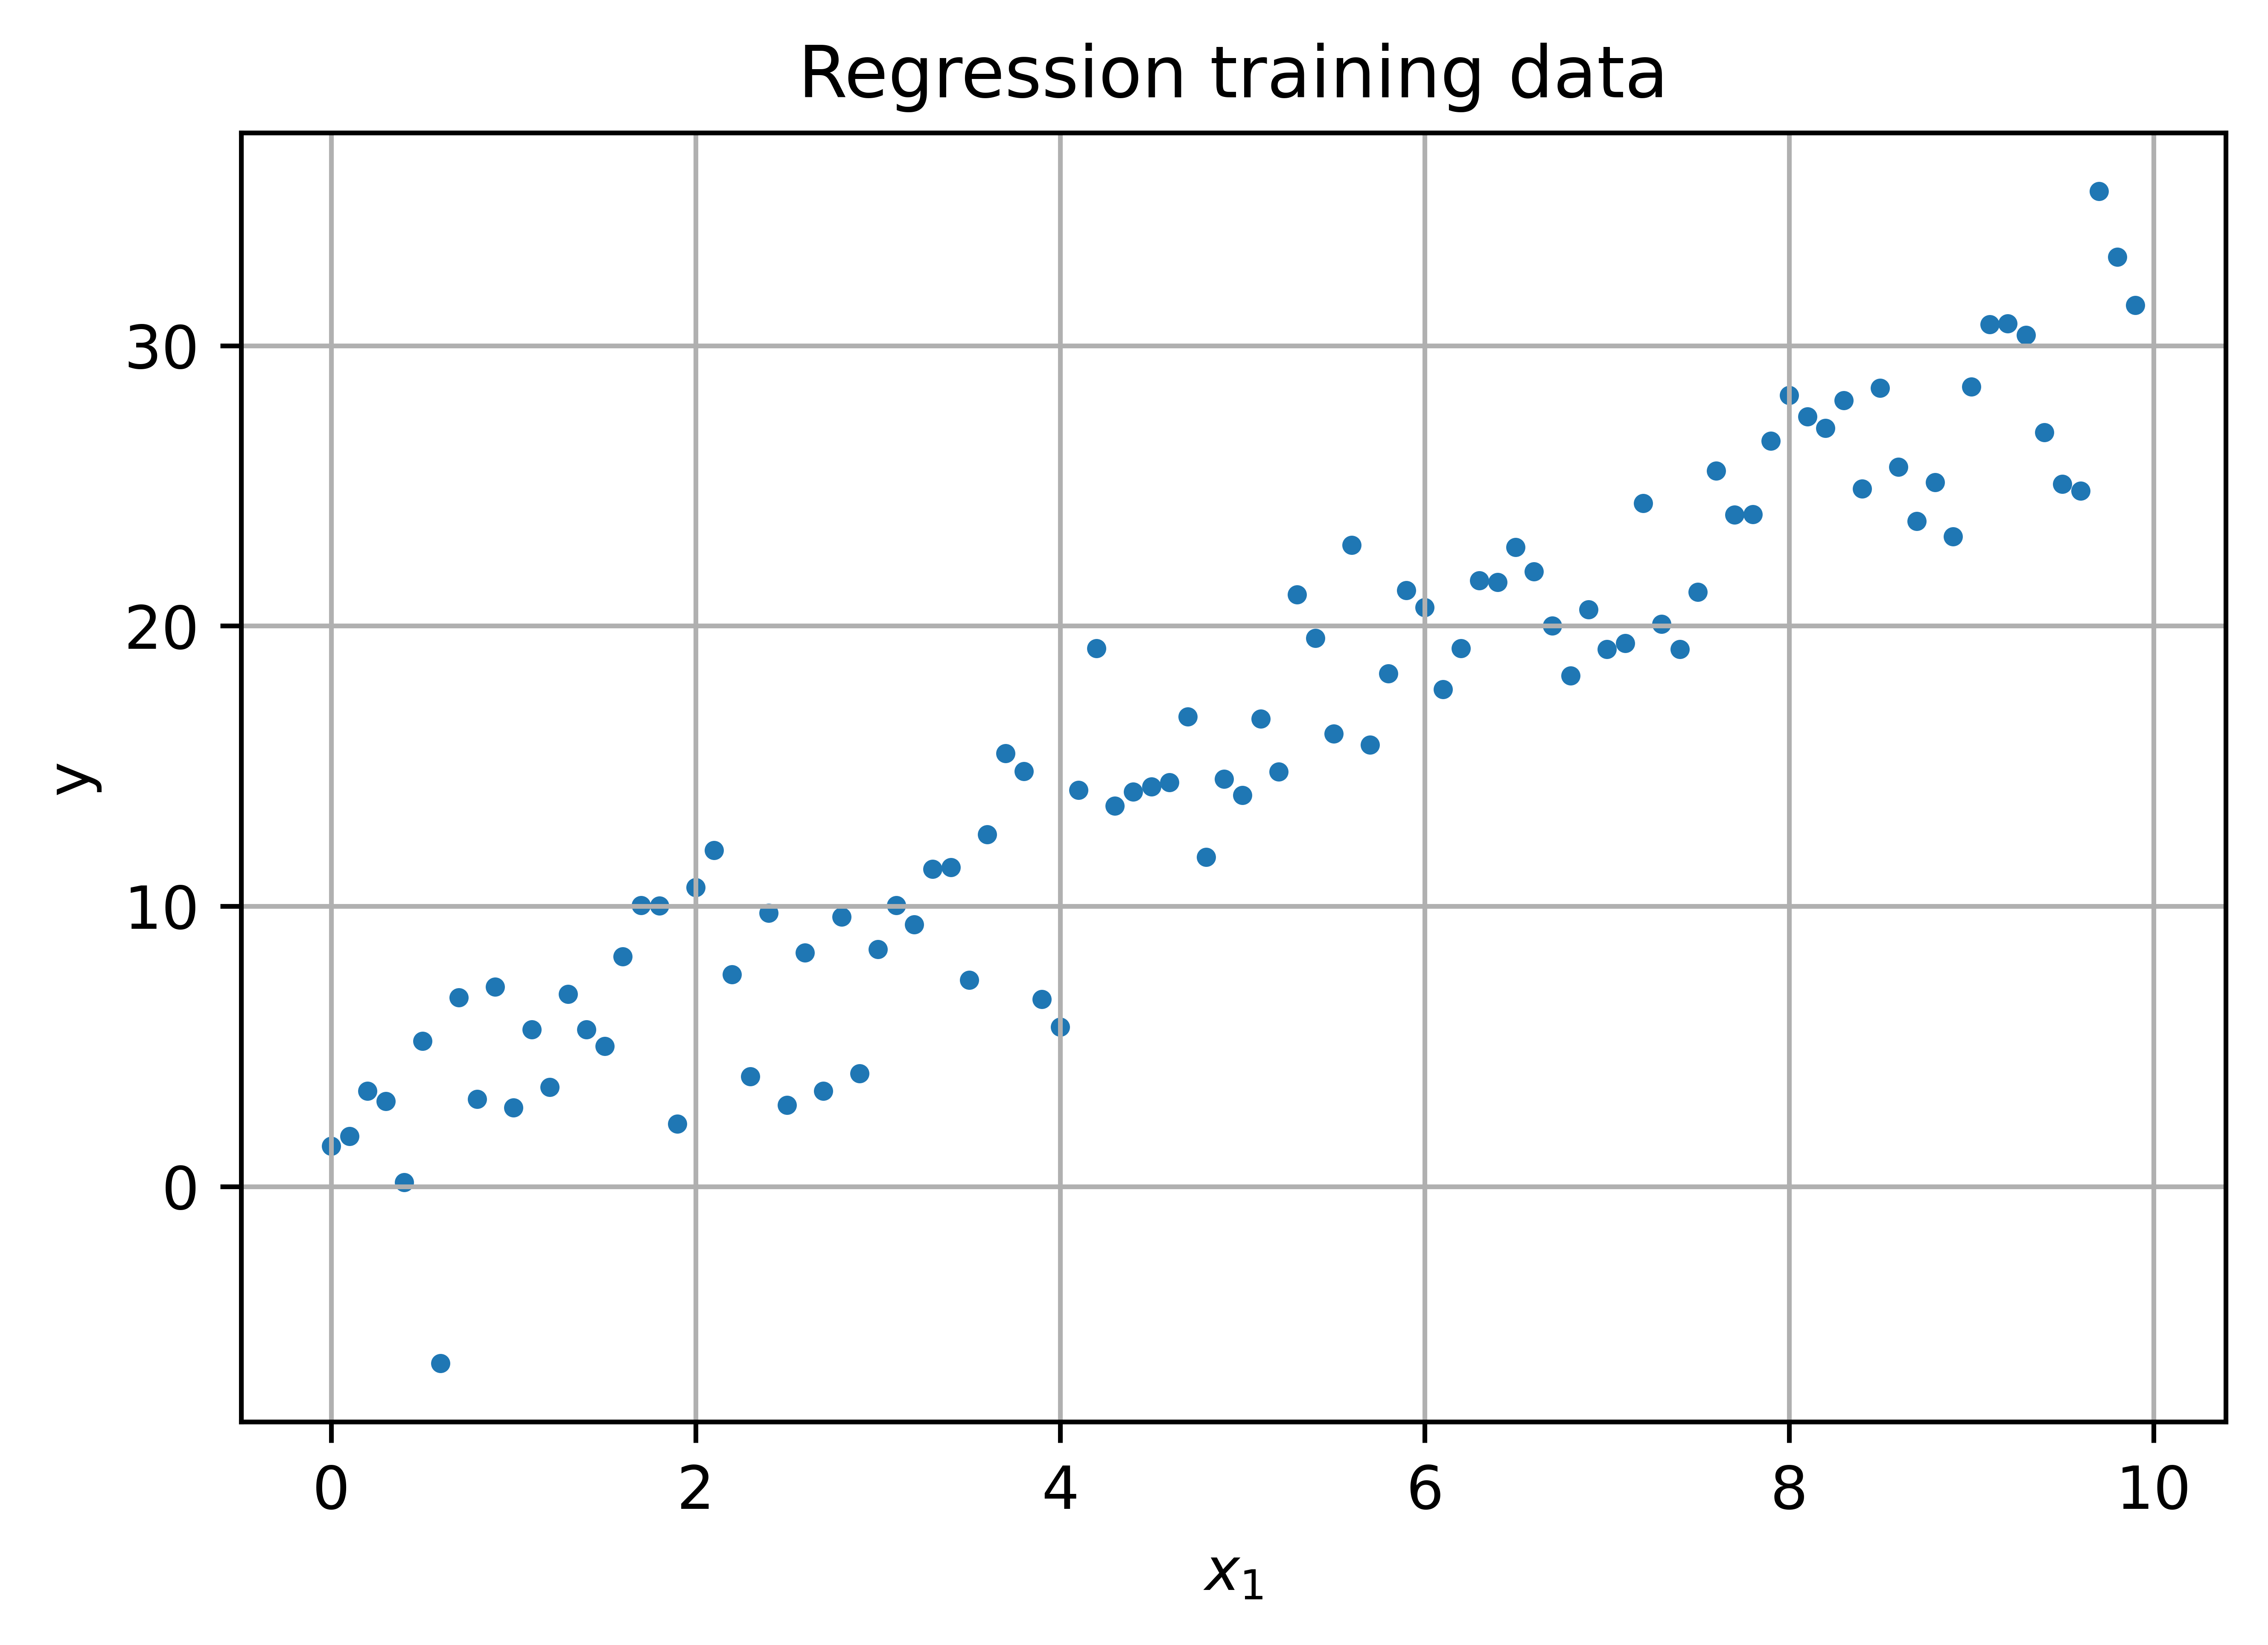
\includegraphics[width=70mm,scale=0.5]{images/regression_images/Regression_Training_Data.png}
        
            \caption*{In this example, you have one input (x-axis), and you want to \textbf{predict} the output (y-axis) based on that. These points are the dataset you want to \textbf{learn} to match.}
        \end{figure}
        
    \subsection{Converting our data}
    
        Often, our data will not be in the right format - maybe we have a car brand, or a color as a variable.
        
        This requires converting this data into real numbers. We do this using something called a \textbf{feature} transformation.\\
        
        \begin{definition}
            A \vocab{feature} is one distinct piece of \gren{information} in our input.
            
            A \vocab{feature transformation} takes those pieces of information, and \purp{transforms} them into something more \gren{useful} - often a better data type or format.
            
            Sometimes, we use it on already-valid formats to find \purp{new patterns} in data.
        \end{definition}
        
        \miniex You have three car brands. Instead of representing them normally, you instead turn them into vectors: 
        
        \begin{equation}
            \text{Brand A }=
            \begin{bmatrix}
              1 \\ 0 \\ 0
            \end{bmatrix},
            \;\;\;\;
            \text{Brand B }=
            \begin{bmatrix}
              0 \\ 1 \\ 0
            \end{bmatrix},
            \;\;\;\;
            \text{Brand C }=
            \begin{bmatrix}
              0 \\ 0 \\ 1
            \end{bmatrix}
        \end{equation}
        \note{This particular feature transformation is called \textbf{one-hot encoding}! We'll return to it later.}
        
        We do our feature transformation with a function: we often notate this function as $\varphi(x)$. 
        
        There are many different feature transformations for different needs. We will come back to this in a later chapter. 
        
        For now, we will simply assume that all of our inputs $x$ are already in $\RR^d$ (vectors of real numbers).
        
    \subsection{Our dataset}
    
        Regression is \textbf{supervised}, meaning we have training data with a correct output included: we have an "answer key" to a practice quiz.
        
        We want to pair up inputs with their correct outputs, so we'll write our first data point as 
        
        \begin{equation*}
            \left( \ex{x}{1}, \ex{y}{1} \right)
        \end{equation*}
        \note{Remember that the superscript tells us that this is the 1st data point.}
        
        And so we have a set of $n$ data points, $\dataTrain$:
        
        \begin{equation*}
            \dataTrain = 
            \left\{  
            \left(\ex{x}{1}, \ex{y}{1}\right), \dots,
            \left(\ex{x}{n}, \ex{y}{n}\right)
            \right\}
        \end{equation*}
        
    \subsection{Measuring our performance}
        
        In the last chapter, we discussed that we use our past \textbf{training data} to learn a good \textbf{model} for our future \textbf{testing data}.
        
        So, even though the training data is what we have in front of us, the \textbf{testing data} is what we care the most about. We want our machine to handle new situations.
        
        We'll assume our data are \textbf{IID}, so that we can \textbf{learn} and \textbf{generalize} effectively. And we'll evaluate ourselves using a \textbf{loss function} $\loss$, a measure of how poorly our model is running.
        
        We care about \textbf{expected loss}, so we'll take an \red{average}. We'll start with our training data, so we call it \vocab{training error}:\\
        
        \begin{kequation}
        
        \vocab{Training Error} is written as:
        
            \begin{equation}
                \trainerr(h) = \red{ \frac{1}{n}  \sum_{i=1}^n } \ex{Loss}{i} = 
                \frac{1}{n}  \sum_{i=1}^n \loss \left( \pur{ h(\ex{x}{i}), \ex{y}{i} } \right)
            \end{equation}
        \end{kequation}
        
        
        Notice that we treat this error as a function of $h$, our hypothesis - our \textbf{hypothesis} is what we're \textbf{adjusting} to try to improve the error.\\
        
        \begin{clarification}
            $\vocab{h}$ is a \gren{function} that takes a \gren{variable}, $x$, as its input. This is the usual format.
            
            \vocab{$\trainerr$} is also a \redd{function}, but it takes in $h$, a \redd{different function}, as an input!
            
            That means one function is using another function as an input. This can sometimes cause confusion.
            
            Make sure to keep track of the difference as you go through this chapter - the idea will come back later.
        \end{clarification}
        
    \subsection{Learning to Generalize}
        
        Our goal, though, is to perform well on testing data: to be able to \textbf{generalize} to data we haven't seen before.
        
        So, let's define \vocab{test error}. This time, we have $m$ new data points.
        
        \begin{equation}
            \testerr(h) = \frac{1}{\red{m}}  \sum_i  \loss \left( h(\ex{x}{i}), \ex{y}{i} \right) 
        \end{equation}
        
        We'll start counting from $n+1$ because we've already used the first $n$ points when training.\\
        
        \begin{kequation}
        
            \vocab{Testing Error} is written as:
            
            \begin{equation}
                \testerr(h) =
                \frac{1}{m}  \sum_{i\purp{=n+1}}^{\purp{n+m}} \loss \left( h(\ex{x}{i}), \ex{y}{i} \right) 
            \end{equation}
        \end{kequation}
        
        
        We want to minimize \textbf{test error}, but by definition of "data we haven't seen before", we can't use it to design our hypothesis.
        
        So, for now, the next best thing to "minimize test error" is "\textbf{minimize training error}", while doing our best to help our hypothesis \textbf{generalize}. We'll discuss how to do that.

\pagebreak
%%%%%%%%%%%%%%%%%%%%%%%%%%%%%%%%%%%%%%%%%%%%%%%%%%%%%%%%%%%%%%%%%%%%%%%%%%%%%%%%%%%%%%%%%%%

\section{Regression as an optimization problem}
    
    We've mentioned that we want to make our loss (error) as low as we can: we want to \textbf{minimize} it. This is a form of \textbf{optimization} - getting the best results from our system.
    \note{Lot of research has gone into solving optimization problems!}
    
    Here, we'll introduce some of the terms and notation of optimization.
    
    \subsection{Objective Function}
    
        Our goal is to minimize our loss. But, \textbf{training loss} is not our main goal: to compensate for that, we might include other terms to make it more \textbf{general}.
        \note{In later sections, we will introduce something called a \textbf{regularizer} to do just that!}
        
        To distinguish between our \textbf{loss} versus our overall goal, we will define an \textbf{objective} function.\\
        
        \begin{definition}
            An \vocab{objective function} is the function we are \purp{optimizing} for: usually, this means that our goal is \purp{minimizing} it.
            
            This term usually contains the \gren{loss}, and sometimes, a \gren{regularizer}.
            
            We minimize our objective function using our \gren{parameters} $\Theta$, so we take that as an input: \purp{J($\Theta$)}
        \end{definition}
        
        \note{We will be seeing a lot of $\Theta$ for a while.}
        
    \subsection{Parts of an Objective Function}
    
        For now, we will just consider loss, so our \textbf{objective function} will be the same as our \textbf{training error}, dependent only on the \textbf{loss function}.
        
        Since we are focusing more on $\Theta$, we'll replace $h(\ex{x}{i})$ with \blu{$h(\ex{x}{i}; \Theta)$}:
        
        \begin{equation*}
            J(\Theta) = \text{Training Error} = 
            \frac{1}{n}  \sum_{i=1}^n \loss ( h(\ex{x}{i}; \blu{\Theta}), \ex{y}{i} ) 
        \end{equation*}
        
        
        
        But once we introduce the \textbf{regularizer} \redd{$R(\Theta)$} to improve \textbf{generalization}, we'll add that term:
        
        \begin{equation*}
            J(\Theta) = \text{Training Error} + \red{\text{Regularizer}}
        \end{equation*}
        
        We will discuss this term in a later section; don't worry about it for now.
        
        We'll also include a scaling factor \blu{$\lambda$} so we can control this term:\\
        
        \begin{kequation}
            
            In general, we write the \vocab{objective function} as:
            
            \begin{equation*}
                J(\Theta) =
                \left( 
                \frac{1}{n}  \sum_{i=1}^n \loss ( h(\ex{x}{i}; \Theta), \ex{y}{i} ) 
                \right)
                +
                \blu{\lambda} \red{ R(\Theta)}
        \end{equation*}
        \end{kequation}
        
        
        In the long run, this is the function we want to \textbf{optimize}.
        
        Notice that our objective function depends on our training data $\data$ as well: what data we have affects what the best result is.
        
        Just like how we can use $h(x;\Theta)$, we'll use the same notation here: \redd{$J(\Theta;\data)$}
        
        $\Theta$ is our "main" input variable, but if we switch out our data $\data$, we would get a different result.\\
        
        \begin{clarification}
           Students often get confused by the fact that our \purp{objective function} $J$ is a function of $\Theta$, while \purp{training error} $\trainerr$ is a function of $h$.
            
            This may seem strange: if \purp{training error} is included in the \purp{objective function}, why have different variables?
            
            The difference is that \purp{training error} is \gren{more general} than the \purp{objective function}, and \purp{$h$} is \gren{more general} than \purp{$\Theta$}.
            
            \begin{itemize}
                \item \purp{Training error} can be used for a \gren{non-parametric model}. Since we don't know if we have parameters, we can't assume $\Theta$, our vector of \gren{parameters}. So, we use $h$.
                
                \item Our \purp{objective function} \gren{assumes} we have parameters $\Theta$: since we want to optimize with $\Theta$, we use it instead.
            \end{itemize}
            
        \end{clarification}
        
    \subsection{Minimization Notation}
        
        Our goal is to minimize $J$ by adjusting $\Theta$. If we accomplish this, there are two questions we can ask ourselves, and some corresponding notation.
        
        To show our point, we'll use the following example:
        
        \miniex Take $f(x)=(x-1)^2$. The minimum output is 0, which happens at $x=1$. So, we have a minimum at $(1, 0)$.
        
        \begin{itemize}
            \item What is the \textbf{minimium} value of $J$ we can find \textbf{by adjusting $\Theta$}?
        \end{itemize}
        
        \begin{notation}
            The \vocab{min function} gives you the \gren{minimum output} of a function we get by adjusting one chosen \purp{variable}.
            
            \begin{equation*}
                \min_{ \pur{ \Theta } }{ \grn{ J(\Theta) } }
            \end{equation*}
            
            The \gren{function we want to minimize} is written to the right, while the \purp{variable we adjust} is written below.
        
        \end{notation}
        
        \miniex 
        
        \begin{equation}
            \min_x{ \red{(x-1)^2} } = \red{0}
        \end{equation}
        
        \begin{itemize}
            \item What \textbf{value} of $\Theta$ gives us \textbf{minimum} $J$?
        \end{itemize}
        
        \begin{notation}
            The \vocab{argmin function} tells you the value of the \purp{input variable} that gives the \gren{minimum output}.
            
            \begin{equation*}
                \argmin{ \pur{ \Theta } }{ \grn{ J(\Theta) } }
            \end{equation*}
            
            The \gren{function we want to minimize} is written to the right, while the \purp{variable we adjust} is written below.
        
        \end{notation}
        
        \miniex
        
        \begin{equation}
            \argmin{\red{x}}{ (x-1)^2 } = \red{1}
        \end{equation}
        
        Why is it called "argmin"? Well, "argument" is used as another word for "input variable". And our argmin function returns the \textbf{argument} with the \textbf{minimum} output.
        
    \subsection{Optimal Value Notation}
        
        So, we want to know what the best model we want get is, where this model is represented by $\Theta$.\\
        
        \begin{notation}
            We add a \vocab{star} $^*$ to indicate the \purp{optimal} variable choice.
            
            If that variable is $z^*$, you would say it as "$z$-star".
        \end{notation}
        
        \miniex 
        
        \begin{equation}
            x^* = 1 \text{ for the above example.}
        \end{equation}
        
        So, if we want optimal $\Theta$, we're looking for:\\
        
        \begin{kequation}
        
            Our \vocab{optimal parameter} vector is written as 
            
            \begin{equation*}
                \Theta^* = \argmin{ \Theta  }{  J(\Theta)  }
            \end{equation*}
        \end{kequation}
        


\pagebreak
%%%%%%%%%%%%%%%%%%%%%%%%%%%%%%%%%%%%%%%%%%%%%%%%%%%%%%%%%%%%%%%%%%%%%%%%%%%%%%%%%%%%%%%%%%%

\section{Linear Regression}

    Now that we understand the problem of \textbf{regression}, and the concept of \textbf{optimizing} over it, we can pick a concrete example.
    
    We want a function that can use information to \textbf{predict} outputs.
    
    \subsection{The Linear Model, 1-D}
    
        We'll start off small: we have one variable, and something we want to predict. And we'll pick the simplest pattern we can:

        \begin{equation}
            y = mx+b
        \end{equation}
        
        A linear equation: $m$ tells us how much our input affects our output. $b$ accounts for everything unrelated to $x$: what is $y$ when $x=0$?
        
        $b$ and $m$ are our parameters: that means they're part of $\Theta$. We'll rename them $\theta_0$ and $\theta_1$. 
        
        \begin{equation}
            h(x) = \red{\theta_1} x + \red{\theta_0}
        \end{equation}
        
    \subsection{The Linear Model, 2-D}
    
        We want to have \textbf{multiple} input variables: $x$ will be a \textbf{vector}, not a number. So, for our above example, we'll \textbf{replace} $x$ with $x_1$.
        
        \begin{equation}
            h(x) = \theta_1 \red{x_1} + \theta_0
        \end{equation}
        
        The simplest way to include $x_2$ by just \textbf{adding} it. We have a scaling factor $\theta_1$ for $x_1$, so we'll give $x_2$ its own \textbf{parameter}, $\theta_2$:
        \note{If $\theta_1$ is the "slope" for $x_1$, $\theta_2$ is the "slope" for $x_2$.}
        
        \begin{equation}
            h(x) = \red{\theta_2 x_2} + \theta_1 x_1 + \theta_0
        \end{equation}
        
    \subsection{The Linear Model, $d$-D}
    
        You can \textbf{expand} this to $d$ dimensions by simply adding more terms:
        \note{This is the "dimension" of our input space: the \textbf{number} of input variables we have.}
        
        \begin{equation}
            h(x) = \red{\theta_0} + \red{\theta_1}x_1 + \red{\theta_2}x_2 + \red{\theta_3}x_3 + ... + \red{\theta_d}x_d
        \end{equation}
        
    \subsection{The Linear Model using Vectors}
        
        Here, we are \textbf{multiplying} components of $x$ and $\theta$ together, then \textbf{adding}. This looks like a \textbf{dot product}:
        
        \begin{equation}
            h(x) = \theta_0 +
            \red{
                \begin{bmatrix}
                    \theta_1 \\ \theta_2 \\ \vdots \\ \theta_d
                \end{bmatrix}
                \cdot
                \begin{bmatrix}
                    x_1 \\ x_2 \\ \vdots \\ x_d
                \end{bmatrix}
            }
        \end{equation}
        
        If we write this symbolically, we get:
        
        \begin{equation}
            h(x) = \theta_0 + \red{\theta \cdot x} 
        \end{equation}
        
        Unfortunately, we had to leave $\theta_0$ out to make it work. $\theta$ is used for the parameters of our \textbf{dot product}, $\Theta$ is \textbf{all} parameters.\\
        
        \begin{notation}
            We represent the \gren{parameters} of our \purp{linear} equation as $\Theta = (\theta, \theta_0)$.
        \end{notation}
        
        This formula looks similar to $y=mx+b$ again! Only this time, we have \textbf{vectors} instead.
        
        We'll swap out the dot product for \textbf{matrix multiplication}: we'll use matrix multiplication a lot in this chapter, and course.
        \note{One benefit is that we can use \textbf{matrices} instead of just \textbf{vectors}!}\\
        
        \begin{kequation}
            The \vocab{linear regression} hypothesis is written as
            
            \begin{equation*}
                h(x) = \red{ \theta^T x } + \theta_0
            \end{equation*}
        \end{kequation}
        
        \note{Make sure you know what $\theta^T$ is: it's the \textbf{transpose}!}
        
        Remember that, when written out, this looks like:
        
        \begin{equation}
            h(x) = 
            \red{
                \begin{bmatrix}
                    \theta_1 & \theta_2 & \theta_3 & \cdots & \theta_d
                \end{bmatrix}
            }
            \blu{
                \begin{bmatrix}
                    x_1 \\ x_2 \\ x_3 \\ \vdots \\ x_d
                \end{bmatrix}
            }
            + \theta_0
        \end{equation}
        
        This is the \vocab{hypothesis class} of \textbf{linear hypotheses} we will reuse throughout the class.
        
    \subsection{Regression Loss}
    
        We need to decide on our \textbf{loss function} for regression: how \textbf{badly} is our model is performing?
        
        We have an \textbf{actual} output value $a$ that we want to compare to our \textbf{guessed} output $g$. If they're more \textbf{different}, that's worth punishing \textbf{more}. 
        
        $g-a$ is our difference, but we want to punish it being both too \textbf{high} or too \textbf{low}: we'll \textbf{square} the \textbf{difference}.
        
        \begin{equation}
            \loss(g,a) = (g-a)^2
        \end{equation}
        
        Or, if we use $y=a$:
        
        \begin{equation}
            \loss(g,y) = (g-y)^2
        \end{equation}
        
        We call this \vocab{square loss}. It punishes high and low guesses equally, and the punishments become more \textbf{severe} as the \textbf{difference} increases.
        \note{Our slope $2x$ gets larger as we move away from $x=0$.}
        
        We use \textbf{square} distance for a few good reasons:
        
        \begin{itemize}
            \item Always positive: high and low guesses are treated equally.
            \item When we have vectors, we can \textbf{represent} it with a \textbf{dot product} $w \cdot w$, or \textbf{matrix multiplication} $w^T w$: tools we like using.
            \item $\norm{w}$ is not \textbf{smooth}: this isn't good for derivatives! $\norm{w}^2$ \textit{is} smooth.
            \note{ To see this, compare $\abs{x}$ to $x^2$.}
        \end{itemize}
        
    \subsection{Our Goal}
        
        Our goal is to minimize the \textbf{loss} $\loss$ on our data set, using the \textbf{linear} model.
        
        We want the smallest distance between our \textbf{hypothesis} and the \textbf{data points}: we want it as \textbf{close} as possible.
        
        Let's write this into a \textbf{single equation}: $J(\Theta)=J(\theta,\theta_0)$
        
        \begin{equation}
            J(\theta,\theta_0) = \text{Training Loss}
        \end{equation}
        
        Get the equation for \textbf{expected loss}, using $\blu{\ex{}{i}}$ to show which data point we're using in the sum:
        
        \begin{equation}
            J(\theta,\theta_0) = 
            \frac{1}{n}  \sum_{i=1}^n 
            \red{ \loss ( g, } \blu{\ex{y}{i}}  \red{)}
        \end{equation}
        
        Substitute in \textbf{squared loss}:
        
        \begin{equation}
            J(\theta,\theta_0) = 
            \frac{1}{n}  \sum_{i=1}^n 
            \red{ ( g -} \blu{ \ex{y}{i}} \red{)^2 }
        \end{equation}
        
        Our guess is given by our \textbf{hypothesis}, $\red{h(} \blu{\ex{x}{i}} \red{;\Theta)}$
        
        \begin{equation}
            J(\theta,\theta_0) = 
            \frac{1}{n}  \sum_{i=1}^n 
            \left( 
                \red{h(} \blu{\ex{x}{i}} \red{;\Theta)} - \blu{ \ex{y}{i}} 
            \right)^2 
        \end{equation}
        
        And finally, we use our linear model, $\theta^T \blu{\ex{x}{i}}  + \theta_0$.\\
        
        \begin{kequation}
            The \vocab{ordinary least squares} \vocab{objective function} for \vocab{linear regression} is written as 
            \begin{equation}
                J(\theta,\theta_0) = 
                \frac{1}{n}  \sum_{i=1}^n 
                \left( \red{ (\theta^T} \blu{\ex{x}{i}} \red{ + \theta_0) } 
                - \blu{\ex{y}{i}} \right)^2 
            \end{equation}
        \end{kequation}
        
        To clarify:
        
        \begin{equation}
            J(\theta,\theta_0) = 
                        \underbrace{
                            \frac{1}{n}  \sum_{i=1}^n 
                        }_{Averaging}
                        \left( 
                            \underbrace{
                                \red{ (\theta^T} \blu{\ex{x}{i}} \red{ + \theta_0) } 
                            }_{guess}
                            - \underbrace{
                                \blu{\ex{y}{i}}
                            }_{answer}
                        \right)^2 
        \end{equation}
        
        From this, we want to find 
        \note{We now have two parameters in our argmin function, but aside from listing both of them, the notation is the same. We just substituted $\Theta = (\theta, \theta_0)$}
        
        \begin{equation*}
            \theta^*, \theta_0^* = \argmin{\theta, \theta_0}{J(\theta,\theta_0)}
        \end{equation*}
        
    \subsection{Visualizing our Model}
    
        With \textbf{one variable}, we've seen that our linear model simply turns into $\theta_1 x_1  + \theta_0$. As you'd expect, on a plot, this looks like a \textbf{line} in the \textbf{2D plane}.
        
        \begin{figure}[H]
        \centering
            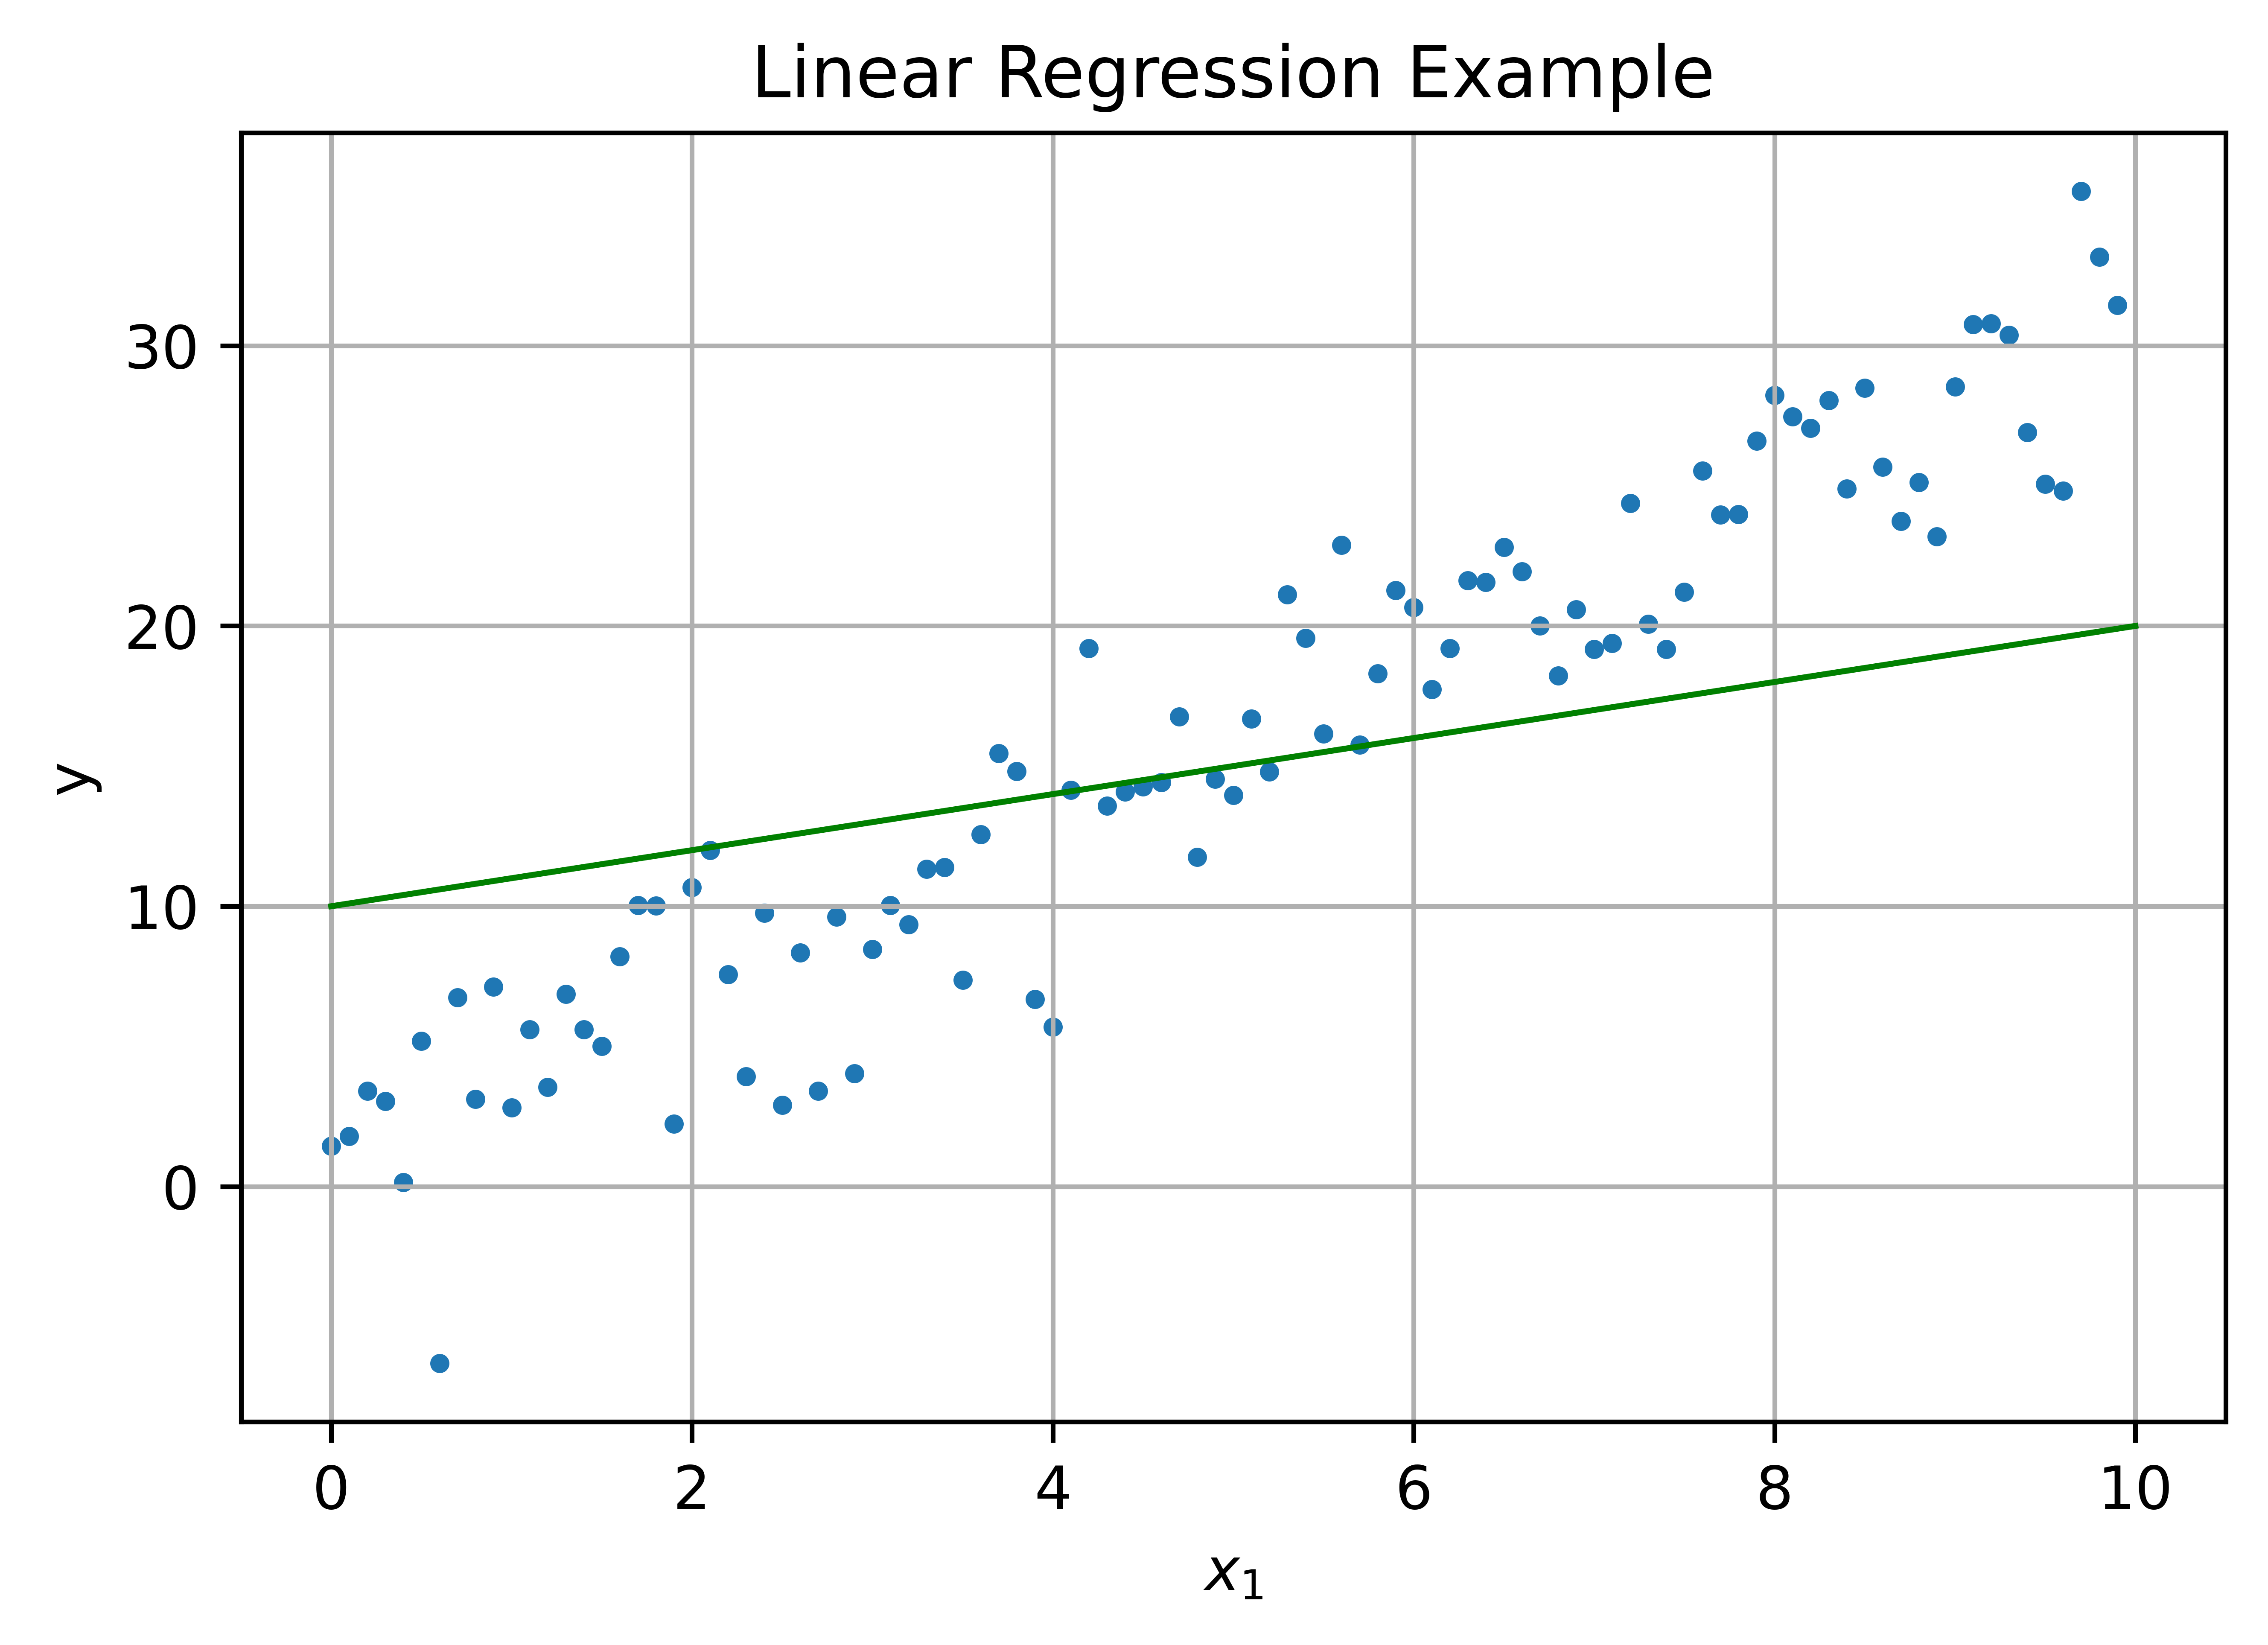
\includegraphics[width=70mm,scale=0.5]{images/regression_images/Regression_Example_Poor_Fit.png}
        
            \caption*{This example of linear regression is not a great fit: $(\theta_0=10, \theta_1=1)$}
        \end{figure}
        
        We're trying to get our line as \textbf{close as possible} to the points, hoping to find a linear pattern. We're \textbf{fitting} our line to the data.
        
        \begin{figure}[H]
        \centering
            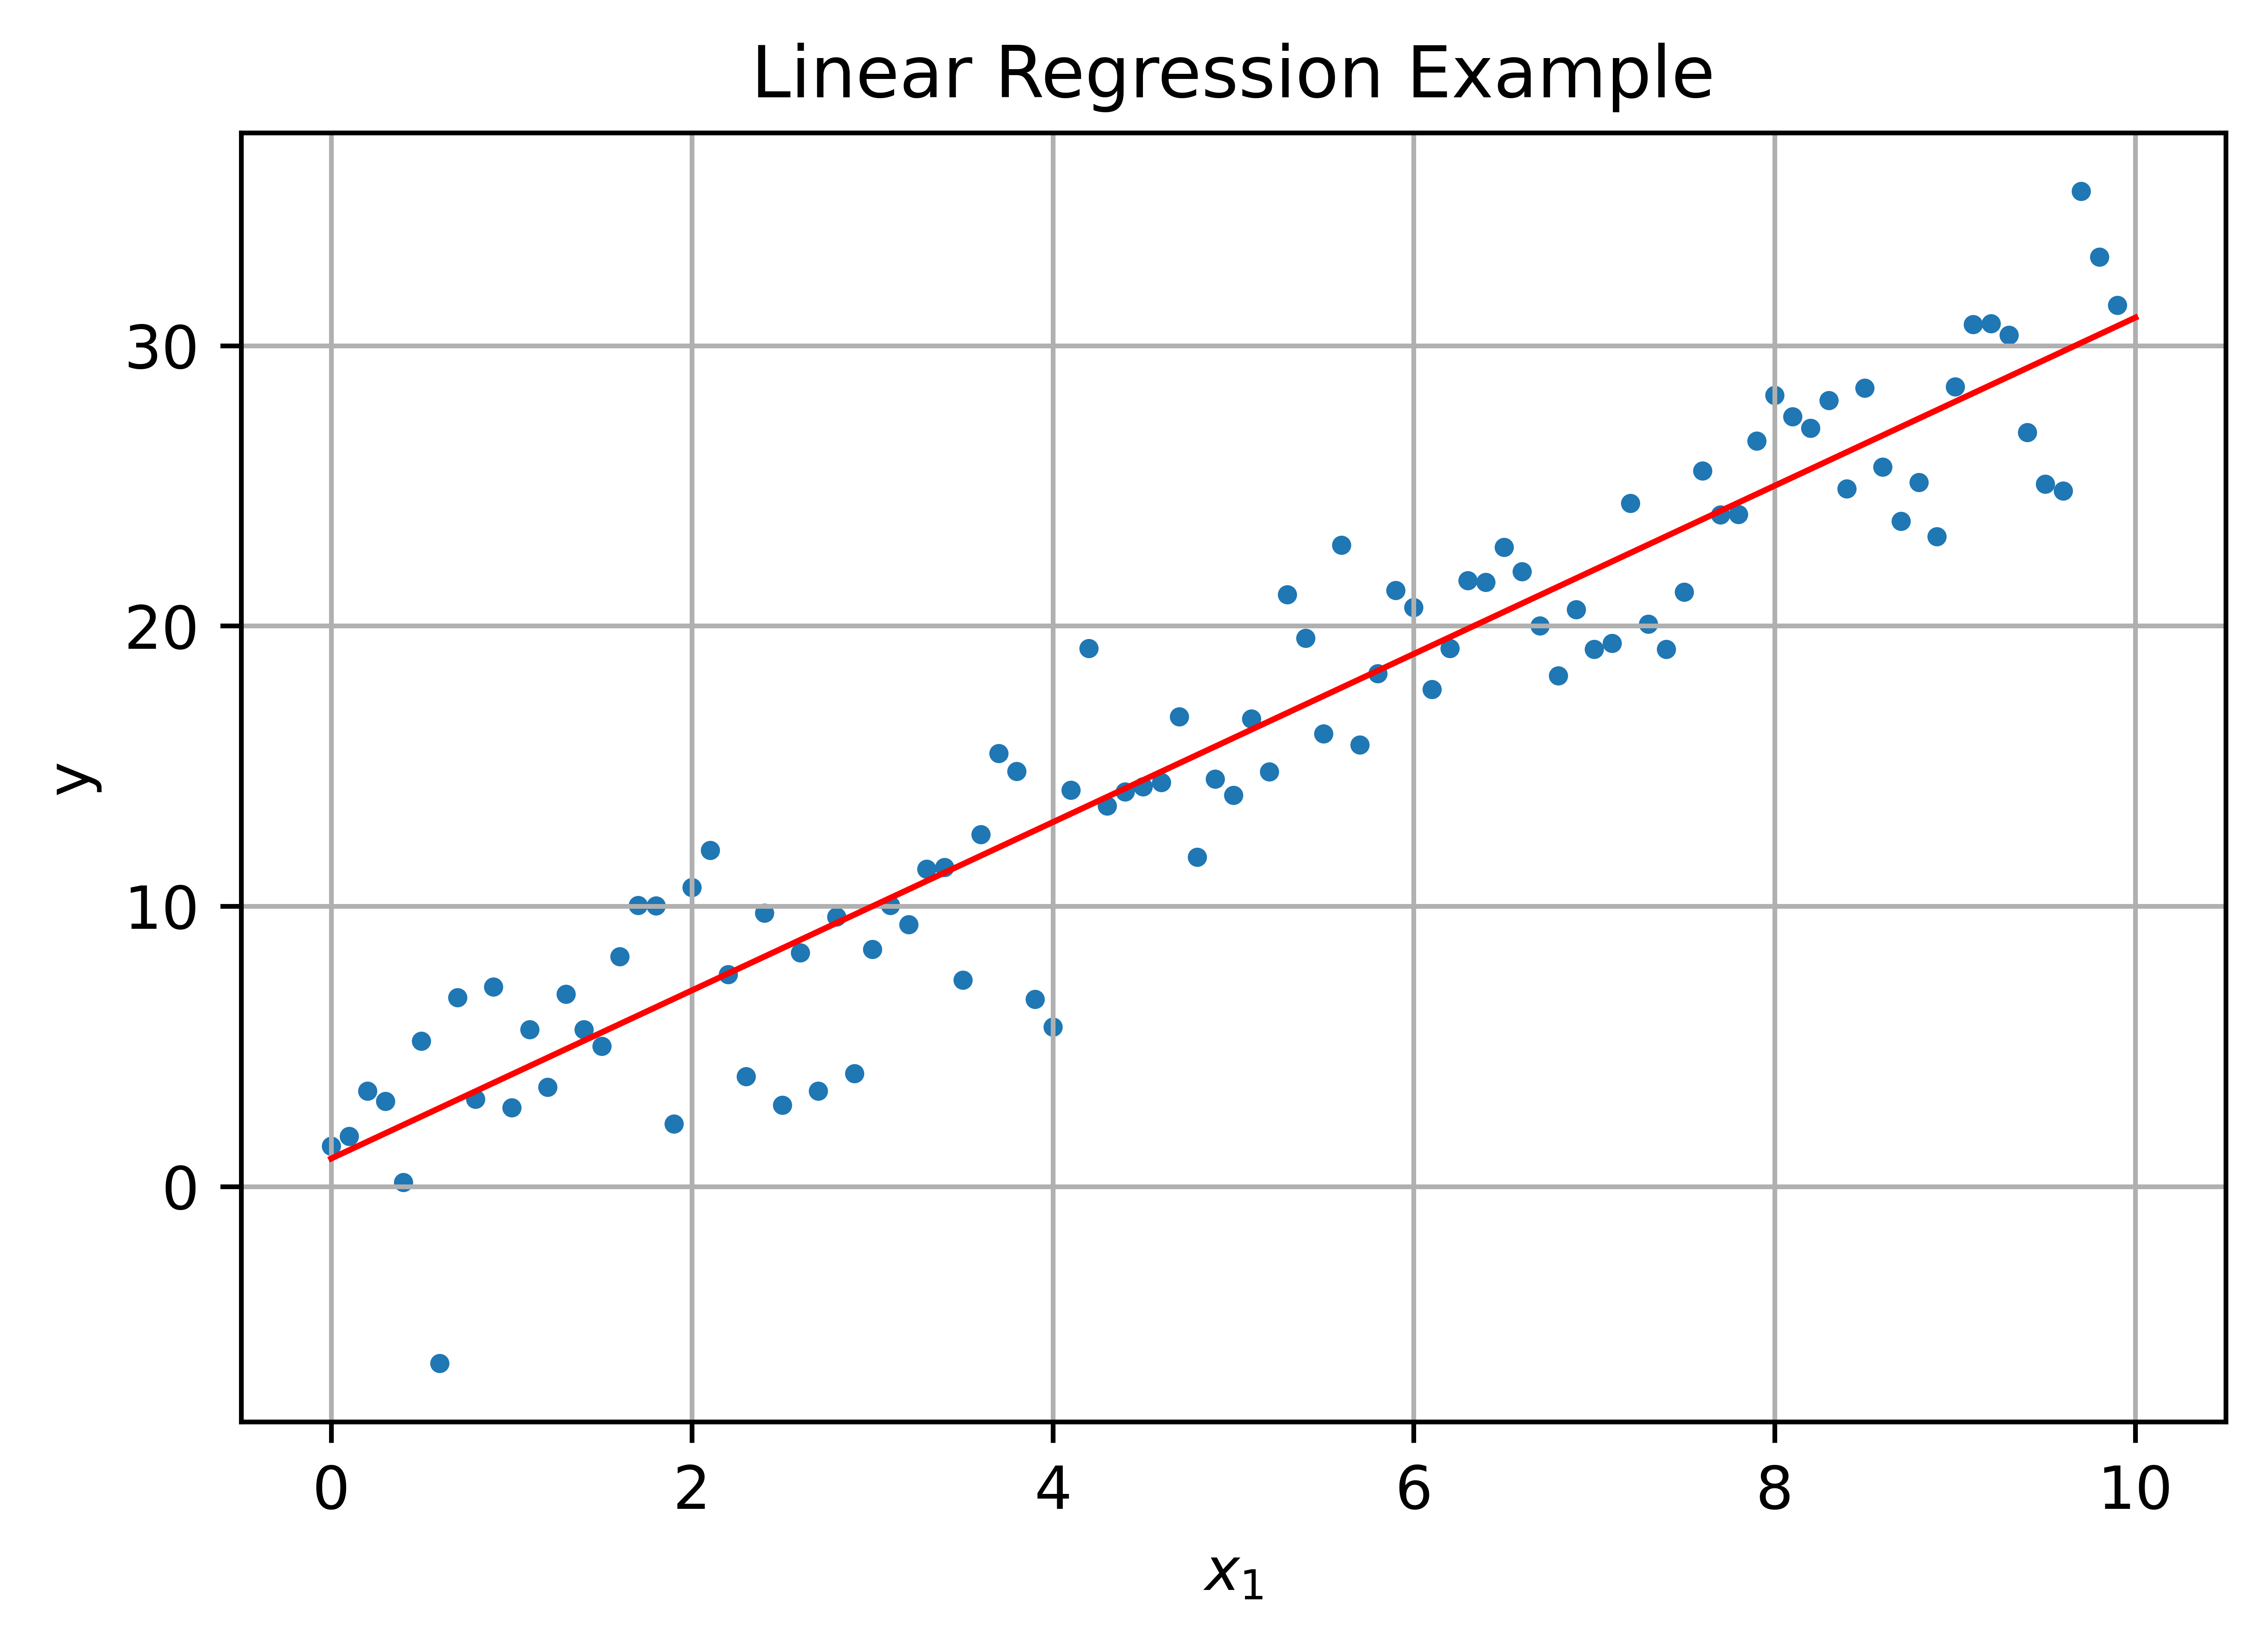
\includegraphics[width=70mm,scale=0.5]{images/regression_images/Regression_Example_Good_Fit.png}
        
            \caption*{This line is much better fitted to the data: $(\theta_0=1, \theta_1=3)$}
        \end{figure}
        
        What does this like if we have \textbf{two} variables? You need a 3D space, with 2 dimensions for the input.
        
        Extending our line into a second dimension, we create a \textbf{plane}.
        
        \begin{figure}[H]
        \centering
            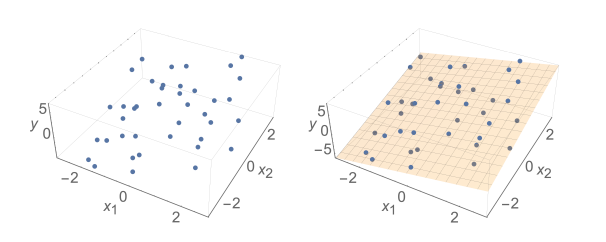
\includegraphics[width=100mm,scale=0.5]{images/regression_images/Regression_Plane.png}
        
            \caption*{This plane is \textbf{fitted} the same way our line was. Notice that $y$ is our \textbf{height}: this is the \textbf{output} of our regression.}
        \end{figure}
        
        Higher-dimension versions are hard to visualize. So, instead, we don't try, and call it a \textbf{hyperplane}.\\
        
        \begin{definition}
            A \vocab{hyperplane} is a \purp{higher-dimensional version} of a \gren{plane} - a \gren{flat} surface that continues on forever.
            
            We use it to represent our \gren{linear} hypothesis for the purpose of \purp{regression}. 
            
            The "\purp{height}" ($\nth{(d+1)}$ dimension) of this \gren{plane} at a certain point represents the \purp{output} of our \gren{linear} hypothesis at that point.
        \end{definition}
        
        Our line was a \textbf{1-D} object in a \textbf{2-D} plane. Our plane was a \textbf{2-D} object in a \textbf{3-D} space. So, our hyperplane is a $d$ dimensional object in a $d+1$ dimensional space.
        
        With this intuition, we can imagine our \textbf{hyperplane} as trying to get as \textbf{close} to all of the data points as it possibly can.
        
    \subsection{Another Interpretation}
    
        There's another, similar way to interpret our model
        
        \begin{equation}
            h(x) = \red{\theta_0} + \red{\theta_1}x_1 + \red{\theta_2}x_2 + \red{\theta_3}x_3 + ... + \red{\theta_d}x_d
        \end{equation}
        
        Before, we took $\theta_k$ as just an \textbf{extension} of the $mx+b$ formula: $\theta_k$ tells us how much $x_k$ affects our output.
        
        However, we can also think about the \textbf{relative} scale of each $\theta_k$: if $\theta_2$ is \textbf{larger} than $\theta_1$, then $x_2$ has a \textbf{stronger} effect on the output than $x_1$.
        
        We can say that $x_2$ \textbf{weighs} more heavily in our calculation: it has more say in the \textbf{result}.
        
        Because of that, we sometimes call $\theta_k$ the \textbf{weight} for $x_k$.\\
        
        \begin{definition}
            A \vocab{weight} is a \gren{parameter} that tells us how \gren{strongly} a variable \purp{influences} our \purp{output}.
            
            It is usually a \purp{scalar} that we \gren{multiply} by our variable.
        \end{definition}

\pagebreak
%%%%%%%%%%%%%%%%%%%%%%%%%%%%%%%%%%%%%%%%%%%%%%%%%%%%%%%%%%%%%%%%%%%%%%%%%%%%%%%%%%%%%%%%%%%

\section{The stupidest possible linear regression algorithm}
    
    So, now we want to try to optimize $J$ based on $\theta$ and $\theta_0$. How do we do that? Let's start as simple as we possibly can.
    
    We can't try \textbf{every} possible $\Theta$, because there are an \textbf{infinite} number of them. Rather than thinking too hard about a possible pattern, or an \textbf{algorithm}, let's just \textbf{randomly} try options.
    
    We'll try \textbf{random} values for $\theta$ and $\theta_0$, and \textbf{pick} whichever option gives us the best result. Seems simple, if inefficient.
    
    Why introduce such a silly algorithm? For two reasons:
    
    \begin{itemize}
        \item It gives us an \textbf{example} of an optimization algorithm that's very \textbf{simple}.
        \item \textbf{Randomly} generated results create a good \textbf{baseline} - more intelligent algorithms can be compared to this one, to see how well we're doing.
    \end{itemize}
    

\pagebreak
%%%%%%%%%%%%%%%%%%%%%%%%%%%%%%%%%%%%%%%%%%%%%%%%%%%%%%%%%%%%%%%%%%%%%%%%%%%%%%%%%%%%%%%%%%%

\section{Analytical solution: ordinary least squares}

    We can do better than randomly \textbf{generate} parameters, though. In fact, in this rare case, we can actually \textbf{solve} for optimal parameters!
    
    \subsection{Trying to Simplify}
        
        Our approach will involve a lot of \textbf{algebra}. Because of that, it's worth it to \textbf{simplify} our formula as much as possible beforehand.
        
        \begin{equation}
            J(\theta,\theta_0) = 
                        \frac{1}{n}  \sum_{i=1}^n 
                        \left( 
                            \underbrace{
                                \red{ (\theta^T} \blu{\ex{x}{i}} \red{ + \theta_0) } 
                            }_{guess}
                            - \underbrace{
                                \blu{\ex{y}{i}}
                            }_{answer}
                        \right)^2 
        \end{equation}
        
        Most parts of this equation can't really be \textbf{simplified}: $y$ and $x$ are just variables, and we can't do anything with the \textbf{sum} without knowing our data points.
        
        But, one thing that was strange is that we \textbf{separated} $\theta_0$ from our other $\theta_k$ terms. Maybe we can \textbf{fix} that.
        
    \subsection{Combining $\theta$ and $\theta_0$}
        
         Let's go back to our \textbf{original} equation for $\red{ (\theta^T} x \red{ + \theta_0) } $, before we switched to \textbf{vectors}.
         \note{We drop the $\ex{}{i}$ notation whenever it isn't necessary, to de-clutter the equations. We only do this when we don't care which data point we're using.}
        
        \begin{equation}
            h(x) = \red{\theta_0} + \red{\theta_1}x_1 + \red{\theta_2}x_2 + \red{\theta_3}x_3 + ... + \red{\theta_d}x_d
        \end{equation}
        
        We converted this into a \textbf{dot product} because each $\theta_n$ term is \textbf{multiplied} by an $x_k$ term, except $\theta_0$.
        
        But if we \textbf{really} want to include $\theta_0$, then could we? We know what's missing: "$\theta_0$ is \textbf{not} multiplied by an $x_k$ term". So... could we get one? Is there a $x_0$ factor we could \textbf{find}?
        
        We need $\theta_0$ to be \textbf{multiplied} by something. Is there something we could "\textbf{factor} out"? How about: $x_0=1$?
        \note{You can always factor out 1 without changing the value!}
        
        \begin{equation}
            h(x) = \red{\theta_0}\blu{x_0} + \red{\theta_1}x_1 + \red{\theta_2}x_2 + \red{\theta_3}x_3 + ... + \red{\theta_d}x_d
        \end{equation}
        
        So, this means we just have to \textbf{append} a 1 to our vector $x$. At the \textbf{same time}, we'll append $\theta_0$ to $\theta$!
        
        \begin{equation}
            x = 
            \begin{bmatrix}
              \red{1} \\ x_1 \\ x_2 \\ x_3 \\ \vdots \\ x_d
            \end{bmatrix},
            \;\;\;\;\;\;\;\;\;\;\;\;\;\;\;
            \theta = 
            \begin{bmatrix}
              \red{\theta_0} \\ \theta_1 \\ \theta_2 \\ \theta_3 \\ \vdots \\ \theta_d
            \end{bmatrix},
            \;\;\;\;\;\;\;\;\;\;\;\;\;\;\;
            h(x) = 
            \begin{bmatrix}
              \red{\theta_0} \\ \theta_1 \\ \theta_2 \\ \theta_3 \\ \vdots \\ \theta_d
            \end{bmatrix}
            \cdot
            \begin{bmatrix}
              \red{1} \\ x_1 \\ x_2 \\ x_3 \\ \vdots \\ x_d
            \end{bmatrix}
        \end{equation}

        We'll write that symbolically, and then apply a transpose.
        
        \begin{equation}
            h(x) = \red{\theta} \cdot x = \blu{ \theta^T x }
        \end{equation}
        
        \begin{concept}
            Sometimes, to simplify our algebra, we can \purp{append} $\theta_0$ to $\theta$. 
            
            In order to do this, we have to \purp{append} a value of 1 to $x$ as well.
            
            Once we do this, we can \gren{write} 
            
            \begin{equation*}
                h(x)=\theta^T x
            \end{equation*}
        \end{concept}
        
        We \textbf{have} to append this 1 to every single $\ex{x}{i}$ in order for this to \textbf{work}. But, now we can treat our parameters as \textbf{one vector}.
    
    \subsection{Summing over data points}
    
        Currently, when using our \textbf{objective} function, we have to \textbf{sum} over \textbf{every} single data point. For the 1D case, this means we have to do:
        
        \begin{equation}
            J = 
            \frac{1}{n}  \sum_{i=1}^n \red{(\theta \ex{x}{i}  - \ex{y}{i} )^2} 
        \end{equation}
        
        This is a bit of a hassle - it \textbf{forces} us to use $\ex{x}{i}$ notation, and we have to be conscious of that \textbf{sum}.
        
        By using \textbf{vectors} above, we were able to work with \textbf{many} variables $\theta_k$ at the same time, making it easier to \textbf{represent} and \textbf{work} with them in the future. 
        
        Can we do the \textbf{same} here - combining many \textbf{data points} into one object, rather than many \textbf{variables}?
    
    \subsection{Summing with Vectors: Row Vectors}
        
        We want to represent \textbf{addition} using \textbf{vectors}. We did that when we were adding $x_k\theta_k$ terms with a \textbf{dot product}.
        
        \begin{equation}
            \red{\theta_0} + \red{\theta_1}x_1 + \red{\theta_2}x_2 + \red{\theta_3}x_3 + ...
            =
            \begin{bmatrix}
              \red{\theta_0} \\ \theta_1 \\ \theta_2 \\ \theta_3 \\ \vdots \\ \theta_d
            \end{bmatrix}
            \cdot
            \begin{bmatrix}
              \red{1} \\ x_1 \\ x_2 \\ x_3 \\ \vdots \\ x_d
            \end{bmatrix}
        \end{equation}
        
        But, dot products also include \textbf{multiplication}. Above, our terms are \textbf{squared}. So, we can multiply $(\theta \ex{x}{i} - \ex{y}{i} )$ times itself!
        
        \begin{equation}
            J = 
            \frac{1}{n}  \sum_{i=1}^n 
            (\theta \ex{x}{i}  - \ex{y}{i} ) (\theta \ex{x}{i}  - \ex{y}{i} )  
        \end{equation}
        
        We'll write $\ex{r}{i} = \theta \ex{x}{i}  - \ex{y}{i}$ to simplify our work. 
        \begin{equation}
            J = \frac{1}{n}  \sum_{i=1}^n
            \ex{r}{i}*\ex{r}{i}
        \end{equation}
        
        In a dot product, we \textbf{add} the \textbf{dimensions} together. So, we'll give each term in our sum its own \textbf{dimension}.
        
        \begin{equation}
            J = \frac{1}{n}  \sum_{i=1}^n
            \ex{r}{i}*\ex{r}{i}
            =
            \frac{1}{n}
            \begin{bmatrix}
              \ex{r}{1} \\ \ex{r}{2} \\ \ex{r}{3} \\ \vdots \\ \ex{r}{n}
            \end{bmatrix}
            \cdot
            \begin{bmatrix}
              \ex{r}{1} \\ \ex{r}{2} \\ \ex{r}{3} \\ \vdots \\ \ex{r}{n}
            \end{bmatrix}
        \end{equation}
        
        We've got a single vector we could call $R$.
        
        We could make it a \textbf{column vector}, but we already use the \textbf{rows} to indicate the \textbf{dimensions}. 
        
        \begin{equation}
            \begin{drcases}
                \theta =
                \begin{bmatrix}
                  \red{\theta_0} \\ \theta_1 \\ \theta_2 \\ \theta_3 \\ \vdots \\ \theta_d
                \end{bmatrix}
            \end{drcases}
            \text{dimensions as rows...}
        \end{equation}
        
        So, let's use \textbf{columns} instead: each \textbf{column} will be a \textbf{data point}: we'll use a \textbf{row vector} $(1 \times n)$. 
        
        \begin{equation}
            R =
            \overbrace{
            \begin{bmatrix}
              \ex{r}{1} & \ex{r}{2} & \ex{r}{3} & \cdots & \ex{r}{n} 
            \end{bmatrix}
            }^{\text{data points as columns!}}
        \end{equation}
        
    \subsection{Going from $x$ to $X$}
    
        We can do the same for our input data $\ex{x}{i}$:\\
        
        \begin{notation}
            We can store all of our 1-D \vocab{data points} in a \vocab{row vector}:
            
            \begin{equation*}
                X =
                \begin{bmatrix}
                  \ex{x}{1} & \ex{x}{2} & \ex{x}{3} & \cdots & \ex{x}{n}
                \end{bmatrix}
            \end{equation*}
            \begin{equation*}
                Y =
                \begin{bmatrix}
                  \ex{y}{1} & \ex{y}{2} & \ex{y}{3} & \cdots & \ex{y}{n}
                \end{bmatrix}
            \end{equation*}
        \end{notation}
        
        We can write our \textbf{objective function} as
        
        \begin{equation}
            J = 
            \frac{1}{n}
            \begin{bmatrix}
              \ex{r}{1} & \ex{r}{2} & \ex{r}{3} & \cdots & \ex{r}{n}
            \end{bmatrix}
            \begin{bmatrix}
              \ex{r}{1} \\ \ex{r}{2} \\ \ex{r}{3} \\ \vdots \\ \ex{r}{n}
            \end{bmatrix}
        \end{equation}
        
        Or more compactly:
        
        \begin{equation}
            J = \frac{1}{n} RR^T
        \end{equation}

        Since we had $\ex{r}{i} = (\theta \ex{x}{i} - \ex{y}{i} )$, we can write 
        
        \begin{equation}
            R = \theta X - Y
        \end{equation}
        \note{Still in the 1D case!}
        
        Let's use this to expand our objective function:\\
        
        \begin{concept}
            In 1-D, we can use row vectors to sum our data points as
            
            \begin{equation*}
                J = \frac{1}{n} (\theta X - Y)(\theta X - Y)^T
            \end{equation*}
        \end{concept}
        
        We've successfully \textbf{removed} the \textbf{sum}!
        
        This format \textbf{stores} all of our \textbf{data points} in \textbf{one object}, just like how we wanted.
        
    \subsection{Putting it together: Matrices}
    
        Now, we have shown both a way to express $x_1, x_2, x_3$ as a single $(d \times 1)$ matrix:
        
        \begin{equation}
            x = 
            \begin{bmatrix}
              x_1 \\ x_2 \\ x_3 \\ \vdots \\ x_d
            \end{bmatrix}
        \end{equation}
        \note{We'll leave off the appended 1 for now.}
        
        And a way to express $\ex{x}{1}, \ex{x}{2}, \ex{x}{3}$ as a single $(1 \times n)$ matrix:
        
        \begin{equation}
            X =
                \begin{bmatrix}
                  \ex{x}{1} & \ex{x}{2} & \ex{x}{3} & \cdots & \ex{x}{n}
                \end{bmatrix}
        \end{equation}
        
        Why not combine them into a single object?\\
        
        \begin{kequation}
            $X$ is our \vocab{input matrix} in the shape \purp{$(d \times n)$} that contains information about both \gren{dimension} and \gren{data points}.
            
            \begin{equation}
                X = 
                    \overbrace{
                        \begin{bmatrix}
                            \ex{x_1}{1} & \cdots  & \ex{x_1}{n} \\
                            \vdots      & \ddots & \vdots      \\
                            \ex{x_d}{1} & \cdots  & \ex{x_d}{n}
                        \end{bmatrix}
                        }^{ n \text{ data points}}
                    \bigggrB{50pt} d \text{ dimensions}
            \end{equation}

        \end{kequation}
        
        If we include the appended 1, we write this as the \purp{$( (d + 1) \times n)$} matrix
        
        \begin{equation}
                X = 
                    \overbrace{
                        \begin{bmatrix}
                            1           & \cdots & 1           \\
                            \ex{x_1}{1} & \cdots  & \ex{x_1}{n} \\
                            \vdots      & \ddots & \vdots      \\
                            \ex{x_d}{1} & \cdots  & \ex{x_d}{n}
                        \end{bmatrix}
                        }^{ n \text{ data points}}
                    \bigggrB{70pt} d+1 \text{ dimensions}
        \end{equation}
        
        Because each data point $\ex{y}{i}$ has only one dimension, it's the same as in the last section:\\
        
        \begin{kequation}
            $Y$ is our \vocab{output matrix} in the shape \purp{$(1 \times n)$} that contains all data points.
            
            \begin{equation*}
                Y = 
                    \begin{bmatrix}
                        \ex{y}{1} & \cdots & \ex{y}{n}
                    \end{bmatrix}
            \end{equation*}
        \end{kequation}
        
        All we have to do is combine our \textbf{equations}: We can use the one in the last section, but because $\theta$ is a matrix, we have to \textbf{transpose} it.
            \note{There was no point in transposing it when it was just a constant!}\\
        
        \begin{kequation}
            Using our \purp{appended} matrix, we can write our \gren{objective function} for \purp{multiple} variables and \purp{multiple} data points as
            
            \begin{equation*}
                J = \frac{1}{n}
                    \left( \red{ \theta^T X - Y} \right)
                    \left( \red{ \theta^T X - Y} \right)^T
            \end{equation*}
        \end{kequation}
        
        It is important to \textbf{remember} the \textbf{shape} of our objects, as well.\\
        
        \begin{concept}
            Our matrices have the shapes:
            
            \begin{itemize}
                \item $X$:        $(d \times n)$ - matrix
                \item $Y$:        $(1 \times n)$ - row vector\\
                
                \item $\theta$:   $(d \times 1)$ - column vector
                \item $\theta_0$: $(1 \times 1)$ - scalar\\
                
                \item $J$:        $(1 \times 1)$ - scalar
            \end{itemize}
            
            If we combine $\theta_0$ into $\theta$, replace every use of $d$ with $d+1$.
            
        \end{concept}
        
        \note{Notice that these shapes make sense for our above equation! Try working through the matrix multiplication to verify this.}
        
        These shapes are worth \textbf{memorizing}.
        
    \subsection{Alterate Notation}
    
        One side problem: some ML texts use the \textbf{transpose} of $X$ and $Y$.\\
    
        \begin{notation}
            Some subjects use \vocab{different notation} for \vocab{matrices}. The main difference is that $X$ and $Y$ use their \purp{transpose}, which we'll notate as
        
            \begin{equation*}
                \Xt = X^T \;\;\;\;\;\;\;\; \Yt = Y^T
            \end{equation*}
            
            Thus, our equation above becomes
            
            \begin{equation*}
                J = \frac{1}{n}
                    \left( \red{ \Xt \theta  - \Yt } \right)^T
                    \left( \red{ \Xt \theta  - \Yt } \right) 
            \end{equation*}
        \end{notation}
        
    \subsection{Optimization in 1-D - Calculus Returns!}
    
        Now that we have our \textbf{problem} presented the way we \textbf{want}, we can figure out how to \textbf{optimize} our $\theta$.
        
        For now, we'll revert to \textbf{sum} notation, but we'll come back to our \textbf{matrices} later.
        
        \begin{equation}
            J(\theta) = 
            \frac{1}{n}  \sum_{i=1}^n 
            \left( \red{\theta^T} \blu{\ex{x}{i}}  
            - \blu{\ex{y}{i}} \right)^2 
        \end{equation}
        
        How do we \textbf{optimize} this? Let's just take \textbf{one data point}:
        
        \begin{equation}
            J(\theta) = (\red{ \theta^T x  } - y )^2
        \end{equation}
        
        And we'll start in 1D.
        
        \begin{equation}
            J(\theta) = (\red{\theta x}   - y )^2
        \end{equation}
        
        If we treat $\theta$ like any ordinary \textbf{variable}, this is just a simple function! How would we find the \textbf{minimum}? 
        
        Using \textbf{calculus}! Anywhere there's a local \textbf{minimum}, we typically know the \textbf{derivative} is 0.
        \note{Assuming a "smooth" surface...}
        
        Note that we aren't taking $\deriv{}{x}$: we want to change our \textbf{model}, not our \textbf{data}! So, since $\theta$ represents our \textbf{model}, we'll take $\deriv{}{\theta}$.
        
        \begin{equation}
            J'(\theta) = 2x(\theta x - y ) = 0
        \end{equation}
        
        We just find where the slope is 0, and solve for $\theta$!
        \note{We technically need to prove whether this is minimum, maximum, or neither. For now, we'll assume we have a minimum.}
        
        \begin{equation}
            \theta^* = \frac{y}{x}
        \end{equation}
        
        \begin{concept}
            
            If our function $J(\theta)$ has \vocab{one variable}, we can \gren{explicitly} find \vocab{local minima} by solving for $\theta$ when the \purp{derivative} is zero.
            
            \begin{equation*}
                \deriv{J}{\theta}=0
            \end{equation*}
            
            Then, you check each candidate using the second derivative to see if it is a minimum ($J''(\theta)>0$). In this class we will often be able to ignore this step.
        \end{concept}
        
        \note{This concept is review from 18.01 (Single-variable calculus), but is worth repeating!}
        
    \subsection{Using our sum}
    
        Now, we'll go back to having multiple data points we want to \textbf{average}:
        
        \begin{equation}
            J(\theta) = \frac{1}{n}  \sum_{i=1}^n 
            \left( \theta \blu{\ex{x}{i}}  
            - \blu{\ex{y}{i}} \right)^2 
        \end{equation}
        
        We want to do the same optimization. Thankfully, derivatives are \textbf{linear}: addition and scalar multiplication are not affected!
        \note{Check the prerequisites chapter, chapter 0, for a full definition of linearity.}
        
        \begin{equation}
            J'(\theta) = \frac{1}{n}  \sum_{i=1}^n \red{2 \ex{x}{i} \cdot
            (\theta \ex{x}{i}  - \ex{y}{i} )} = 0
        \end{equation}
        
        And we can \textbf{solve} this just the same way.
        
    \subsection{Optimizing for multiple variables}
    
        Now, the tricky part is working with \textbf{vectors}.
        \note{We'll ignore the averaging and $\ex{}{i}$ notation since that's easy to add on afterwards.}
        
        \begin{equation}
            J(\theta) = (\red{ \theta^T x  } - y )^2
        \end{equation}
        
        We want to \textbf{optimize} this. In the \textbf{one-dimensional} case, we wanted to set the \textbf{derivative} of $J$ to \textbf{zero}, using a single $\theta$ variable. Now, we have \textbf{multiple} variables $\theta_k$ to \textbf{change}.
        
        \textbf{Derivatives} are all about \textbf{change} in variables, and our \textbf{change} $\Delta \theta$ is a \textbf{combination} of changing the different \textbf{components}, $\Delta \theta_k$. 
        
        \begin{equation}
            \Delta \theta =
            \begin{bmatrix}
                \Delta \theta_0 \\ \Delta \theta_1 \\ \Delta \theta_2 \\ \vdots \\ \Delta \theta_d
            \end{bmatrix}
        \end{equation}
        
        So, maybe it would be reasonable to just set \textbf{every} derivative to \textbf{zero}? It turns out, the answer is \textbf{yes}! 
        
        We can show this by using the \textbf{chain rule} definition:
        
        \begin{equation}
            \overbrace{
                \Delta \theta \; \deriv{J}{\theta}} 
            ^{\text{The change in $J$ from $\theta$ overall } }
            \approx 
            \overbrace{
                \Delta \theta_0 \; \pderiv{J}{\theta_0} + \Delta \theta_1 \; \pderiv{J}{\theta_1} + \dots + \Delta \theta_d \; \pderiv{J}{\theta_d}
            }^{\text{The change in $J$ from each $\theta_k$ term} }
        \end{equation}
        
        So, if all the derivatives are zero, the \textbf{overall} derivative is zero.
        \note{This approximation formula becomes exact as the step size shrinks: we go from $\Delta \theta$ to $\dd \theta$.}\\
        
        \begin{concept}
            If our function $J(\theta)$ has \red{$d$} \vocab{different variables} , we can \gren{explicitly} find \vocab{local minima} by getting all of the \purp{equations}
            
            \begin{equation*}
                \pderiv{J}{\theta_0} = 0, \;\;\;
                \pderiv{J}{\theta_1} = 0, \;\;\;
                \pderiv{J}{\theta_2} = 0... \;\;\;
                \pderiv{J}{\theta_d} = 0
            \end{equation*}
            
            Or in general, 
            
            \begin{equation*}
                \pderiv{J}{\theta_k} = 0 \;\;\; \text{ for all k in \{0, 1, 2, ..., d\} }
            \end{equation*}
            
            ...And solving this \purp{system of equations} for the \gren{components} of $\theta$.
            
        \end{concept}
        
        \note{Again, we ignore the second requirement of making sure this isn't a \textbf{maximum} or \textbf{saddle} point.}
        
        The \textbf{solution} to this system of equations will be our \textbf{desired result}, $\theta^*$.
        
    \subsection{Gradient Notation}
    
        Writing it this way can be a \textbf{hassle}. So, we'll continue our tradition of using \textbf{matrix-based} notation to make our lives easier.
        
        You may recognize these \textbf{component-wise} derivatives as part of the "\textbf{multivariable} version" of the derivative: the \textbf{gradient}.\\
        
        \begin{kequation}
            The \textbf{gradient} of $J$ with respect to $\theta$ is
            
            \begin{equation}
                \nabla_\theta J =
                \pderiv{J}{\theta} =
                \begin{bmatrix}
                    \pderivslash{J}{\theta_0} \\
                    \vdots \\
                    \pderivslash{J}{\theta_d}
                \end{bmatrix}
            \end{equation}
        
        \end{kequation}
        
        \note{Note the subscript on the gradient! This emphasizes that our \textbf{space} is the components of $\theta$, not the components of our data $x$.}
        
        For example, our previous approach boiled down to saying
        
        \begin{equation}
            \nabla_\theta J =
            \begin{bmatrix}
                \pderivslash{J}{\theta_0} \\
                \vdots \\
                \pderivslash{J}{\theta_d}
            \end{bmatrix}
            = 
            \begin{bmatrix}
                0 \\
                \vdots \\
                0
            \end{bmatrix}
            =
            0
        \end{equation}
        
        For our purposes, we will simply \textbf{represent} that \textbf{zero vector} with a single 0.\\
        
        \begin{concept}
            
            If our function $J(\theta)$ has a \vocab{vector variable}, we can \gren{explicitly} find \vocab{local minima} by solving for $\theta$ when the \purp{gradient} is \purp{0}.
            
            \begin{equation*}
                \nabla_\theta J=0
            \end{equation*}

        \end{concept}
        
        \note{Ignoring the requirement from earlier! We're assuming it's a minimum.}
        
        This is the form we will be solving. 
        
    \subsection{Matrix Calculus}
    
        Taking derivatives of vectors falls under \textbf{vector calculus}. That would solve our \textbf{above} problem.
        
        But, before, we showed that it's more \textbf{convenient} if we can store these instead as \textbf{matrices}: that way, we don't need the \textbf{sum}. Luckily, we can generalize our work with \textbf{matrix calculus}. 
        
        Below, we will use the alternative notation, to be consistent with the official notes.
        
        \begin{equation}
            J = \frac{1}{n}
                \left( \red{ \Xt \theta  - \Yt } \right)^T
                \left( \red{ \Xt \theta  - \Yt } \right) 
        \end{equation}
        
        We will not show here how to \textbf{find} these derivatives, but the important rules you need to compute our derivatives are in the \textbf{appendix}.
        \note{There's a document explaining vector derivatives coming soon!}
        
        Note that \textbf{matrix} derivatives often look \textbf{similar} to \textbf{traditional} derivatives, but they are \textbf{not the same}. Most often, making this mistake will result in \textbf{shape errors}.
        \note{Sometimes, you can guess a derivative by using the familiar rules and fixing shape errors with transposing/changing multiplication order. But be careful!}
        
        When we take our derivative, we get
        
        \begin{equation}
            \nabla_\theta J = 
                \frac{2}{n} \Xt^T
                \left( \red{ \Xt \theta  - \Yt } \right) 
            =0
        \end{equation}
        
        From here, we just solve for $\theta$ just like in the official notes.\\
        
        \begin{kequation}
        
            The \vocab{solution} for \vocab{OLS optimization} is 
            
            \begin{equation*}
                \theta = 
                \underbrace{ 
                \inv{ \left(  \Xt^T\Xt  \right)  }
                }_{d \times d}
                \underbrace{
                \Xt^T
                }_{d \times n}
                \underbrace{
                \Yt
                }_{n \times 1} 
            \end{equation*}
            
            Or, in our \purp{original} notation,
            
            \begin{equation*}
                \theta = 
                \underbrace{ 
                \inv{ \left(  XX^T  \right)  }
                }_{d \times d}
                \underbrace{
                X
                }_{d \times n}
                \underbrace{
                Y^T
                }_{n \times 1} 
            \end{equation*}
            
        \end{kequation}
        
    And we're done with OLS!

        
\pagebreak
%%%%%%%%%%%%%%%%%%%%%%%%%%%%%%%%%%%%%%%%%%%%%%%%%%%%%%%%%%%%%%%%%%%%%%%%%%%%%%%%%%%%%%%%%%%

\section{Regularization}
    
    So far, we've shown how to make the \textbf{best} model for our \textbf{training data}. But now, we want to move to our \textbf{real} goal: performing well on \textbf{test data}.
    
    This means we want to make a model that is \textbf{general}: it can apply well to \textbf{new data}.
    
    \subsection{Regularizers}
        
        Only focusing on training data is a \textbf{weakness} for our model - if by chance, we have a training data that doesn't \textbf{match} our overall distribution, we are likely to make a \textbf{bad model}.
        
        \miniex You flip \textbf{4 coins}, and get \textbf{3 heads}. You determine that this coin has a \textbf{75\% chance} of landing heads. It turns out this \textbf{isn't true}: it's a fair coin, and you got \textbf{unlucky}.
        \note{You can also increase sample size (flip more times), but for complex problems this isn't always an option!}
        
         We may need a \textbf{second} way to measure our performance: one that focuses \textbf{less} on \textbf{current} performance, and \textbf{more} on predicting how \textbf{generalizable} it is.
        
        We call this type of function a \textbf{regularizer}.\\
        
        \begin{definition}
            A \vocab{regularizer} is an added term to our \gren{loss function} that helps measure how \purp{general} our hypothesis is.
            
            By \gren{optimizing} with this term, we hope to create a model that works better with \purp{new data}.
            
            This function takes in our \purp{vector of parameters} \gren{$\Theta$} as an input: \purp{$R(\Theta)$}
        \end{definition}
        
        \miniex You figure that the coin is \textbf{equally likely} to bias towards heads or tails: even if it's \textbf{weighted}, you don't know \textbf{which way}. So, you start with \textbf{50-50} odds, and \textbf{adjust} that based on evidence.
        \note{Instead of just focusing on the \textbf{specific} data for our coin, we consider how coins act in \textbf{general}.}
        
    \subsection{Regularizer for Regression: Prior Knowledge}
        
        Now, the question is, \textbf{how} do we choose our regularizer? What will make our model more \textbf{general}?
        
        We want to \textbf{resist} the effects of random \textbf{chance}, like in the \textbf{coin} example above. In that example, we improved our guess by starting with a \textbf{prior assumption}.
        
        If you have some \textbf{previous} guess, or past experience, you might have some \textbf{model} you \textbf{expect} to work well: the data has to \textbf{convince} you otherwise.
        
        So, we might consider a model \textbf{more different} from that past one, $\Theta_{\text{prior}}$, to be \textbf{suspicious}, and less likely to be good.\\
        
        \begin{concept}
            If we have a \purp{prior} hypothesis $\Theta_{\text{prior}}$ to work with, we might improve our \purp{new} model by encouraging it to be \gren{closer} to the old one.
            
            \begin{equation*}
                R(\Theta)= \norm{ \Theta - \Theta_{\text{prior}} }^2
            \end{equation*}
            
            We measure how \gren{similar} they are using \vocab{square distance}.
            
        \end{concept}
        
        \miniex You have a \textbf{pretty good} model for \textbf{predicting} company profits, but it isn't perfect. You decide to train a \textbf{better} one, but you expect it to be \textbf{similar} to your old one.
        
        
    \subsection{Regularizer for Regression: No Prior Hypothesis}
    
        But, what if we \textbf{don't have} a prior hypothesis? What if we have \textbf{no clue} what a \textbf{good} solution looks like?
        
        Well, just like in the \textbf{coin} example, we don't expect it to be \textbf{more likely} to be \textbf{weighted} towards heads or tails.
        
        So, even if we \textbf{didn't know} most coins are fair coins, we still would've chosen \textbf{50-50} as our guess.
        
        In this case, as far as we know, every $\theta_k$ term is \textbf{equally likely} to be \textbf{positive or negative} - we have no clue.
        
        So, \textbf{on average}, we could push for it to be \textbf{closer to zero}, so it doesn't drift in any direction too strongly.\\
        
        \begin{kequation}
            In general, our \vocab{regularizer for regression} will be given by \purp{square magnitude} of $\theta$:
            
            \begin{equation*}
                R(\Theta) = \norm{\theta}^2 = \theta \cdot \theta
            \end{equation*}
            
            This approach is called \vocab{Ridge Regression}.
        \end{kequation}
        
        \note{We'll discuss why it's called "ridge" regression once we find our solution.}
        
    \subsection{Why not include $\theta_0$?}
    
        One thing you might immediately notice is that we used the magnitude of $\theta$ instead of $\Theta$: this omits $\theta_0$. Why would we do that?
        
        We'll show that we need to \textbf{allow} the \textbf{offset} to have whatever value works best, and we shouldn't \textbf{punish} it. 
        \note{For simplicity, we won't do any regularization here: we can make our point without it.}
        
        This is best shown with a \textbf{visual} example. Let's take an example with one input $x_1$. So, we have a \textbf{linear} function: \red{$h(x) = \theta_1x_1+\theta_0$}.
        
        \begin{figure}[H]
        \centering
            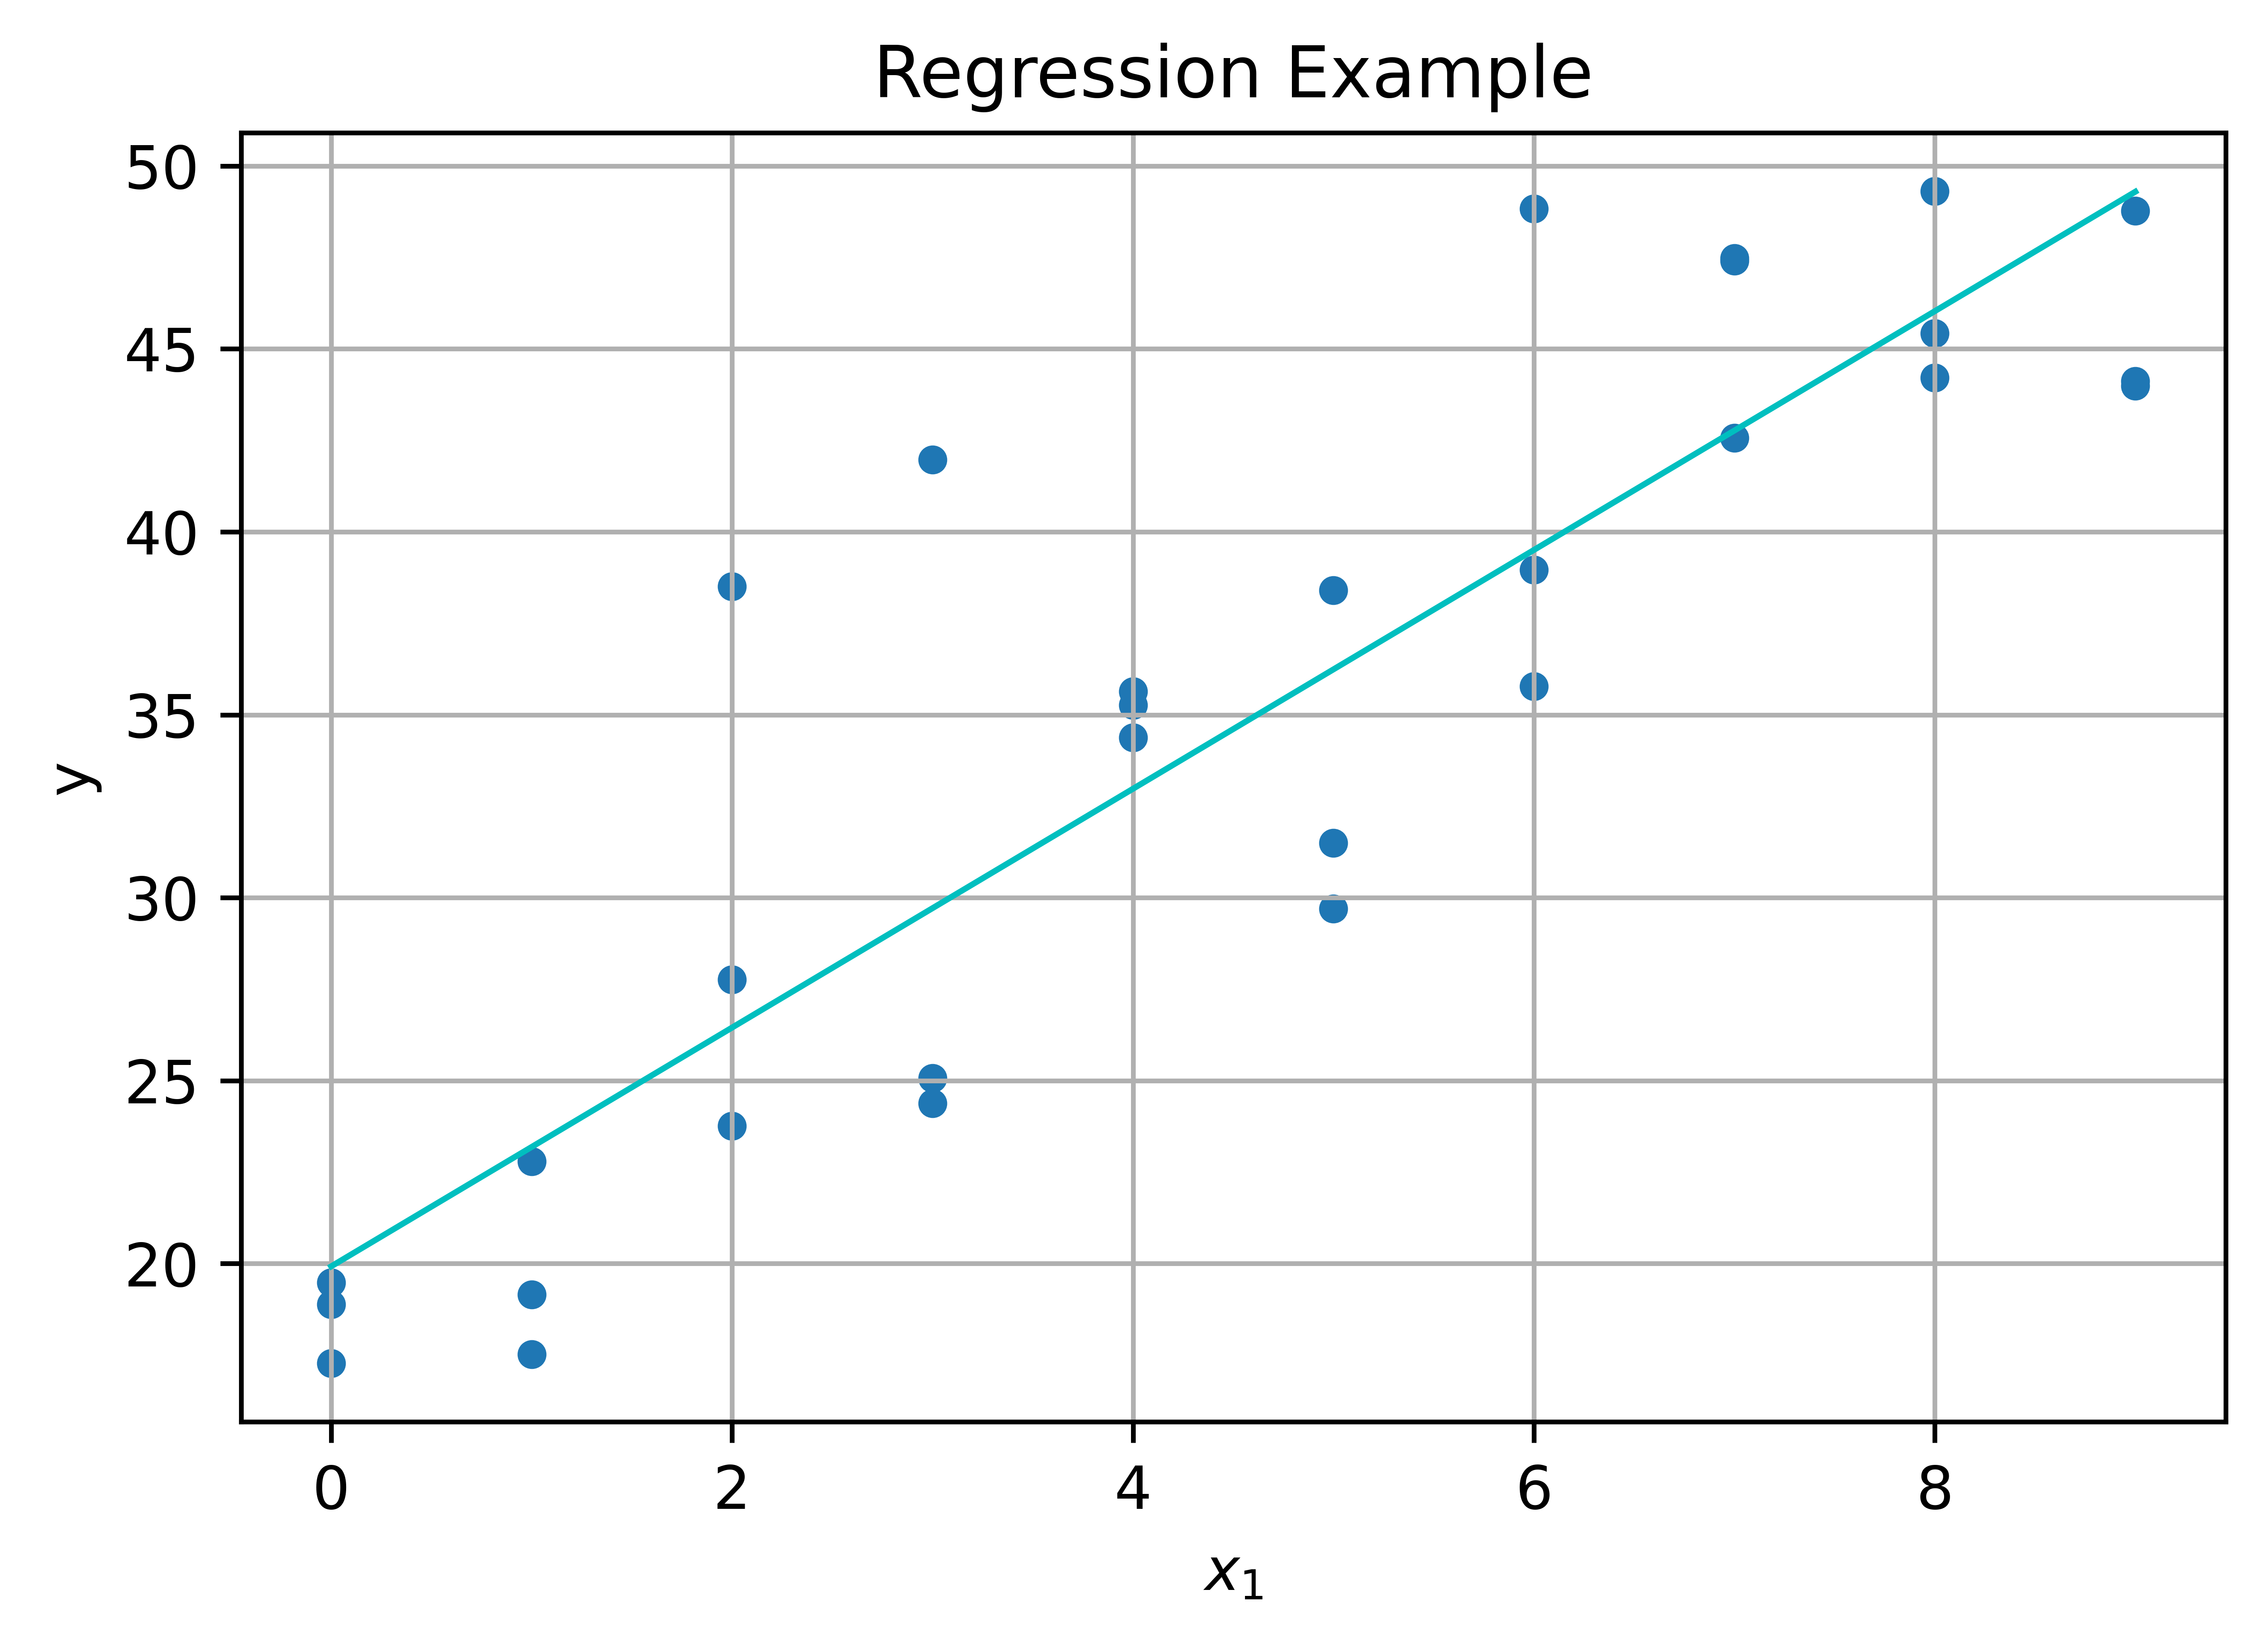
\includegraphics[width=70mm,scale=0.5]{images/regression_images/Regression_Keep_Offset.png}
        
            \caption*{Our regression example.}
        \end{figure}
        
        Let's suppose we \textbf{push} for a \textbf{much lower} (offset) $\theta_0$ term, while keeping everything else the \textbf{same}:
        
        \begin{figure}[H]
        \centering
            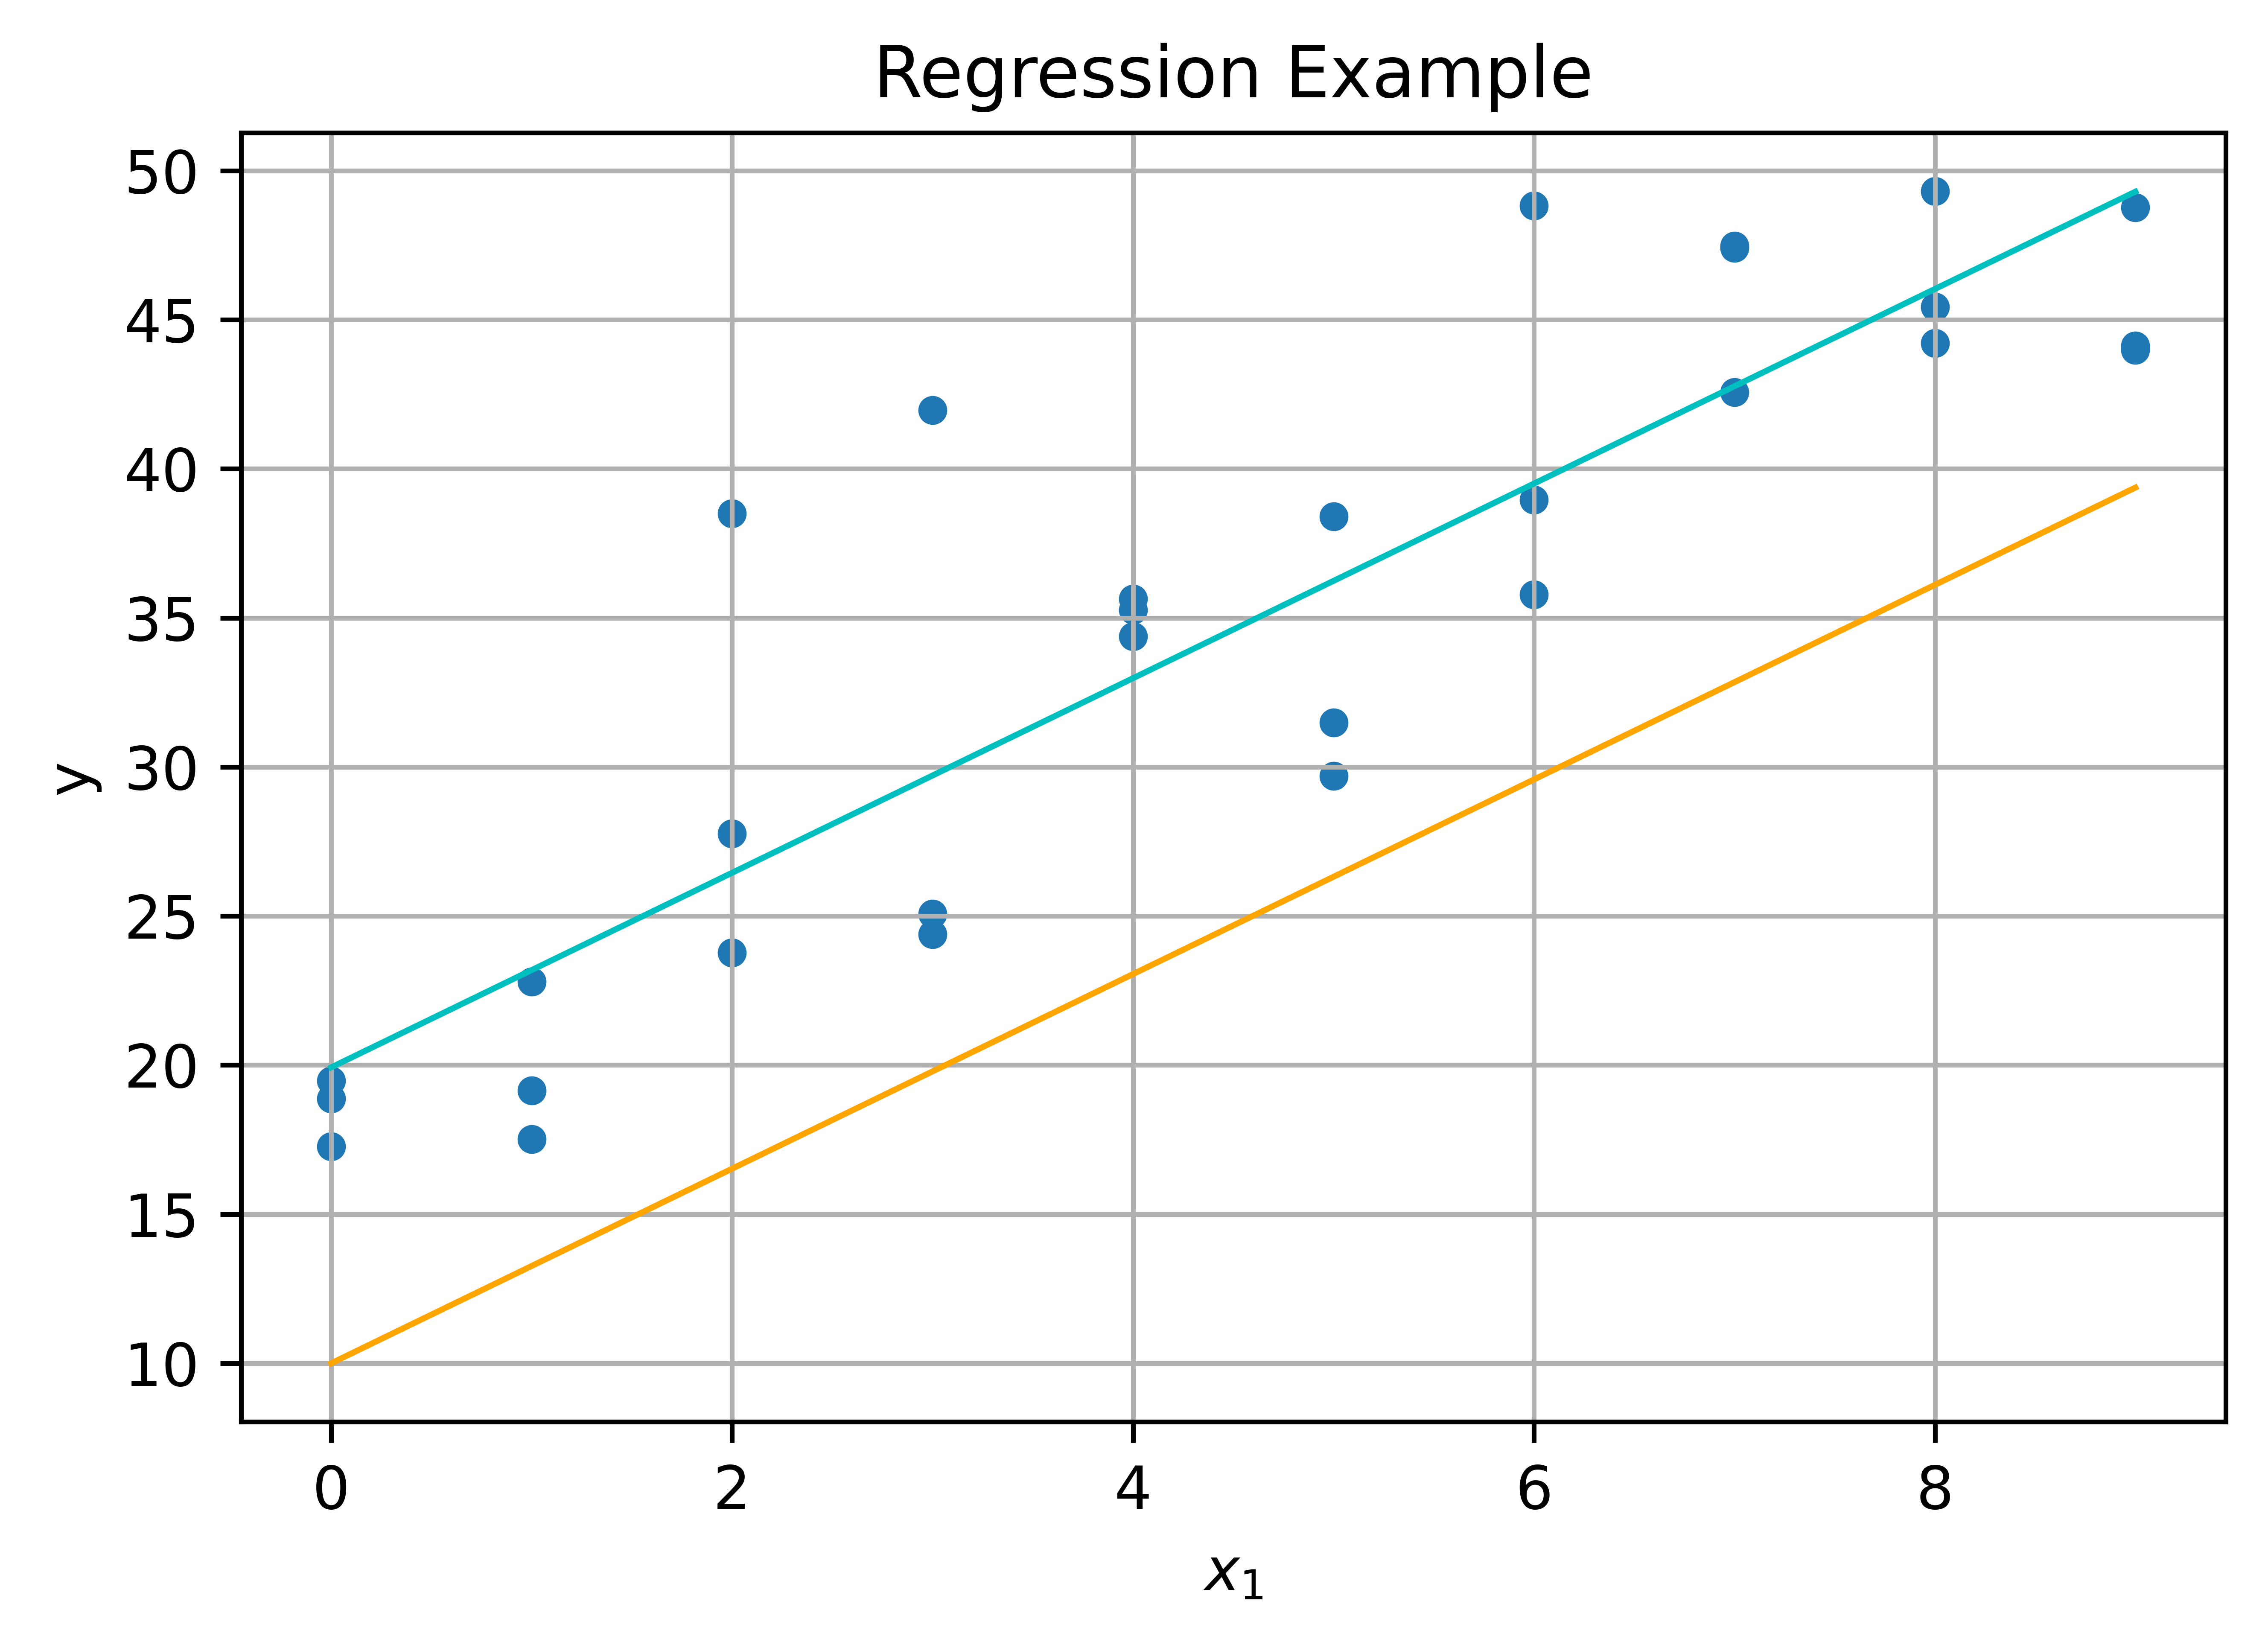
\includegraphics[width=70mm,scale=0.5]{images/regression_images/Regression_Remove_Offset.png}
        
            \caption*{Reducing our offset pulls our line further away from all of our data! That's not helpful.}
        \end{figure}
        \note{And regularizing $\theta_1$ wouldn't make this any better: it would just be flatter.}
        
        This shows that we \textbf{need} our offset! We use it to \textbf{slide} our hyperplane around the space: if all of our data is \textbf{far} from $(0,0)$, we need to be able to \textbf{move} our \textbf{entire line}.
        
        So, we'll keep $\theta_0$ \textbf{separate} and \textbf{allow} it to take whatever value is \textbf{best}.\\
        
        \begin{concept}
            We \purp{do not regularize} our \purp{offset} term, $\theta_0$. 
            
            Instead, we allow $\theta_0$ to \gren{shift} our hyperplane wherever it \gren{needs} to be.
        \end{concept}
        
        The other terms $\theta$ control the \textbf{orientation} of the hyperplane: the \textbf{direction} it is \textbf{facing}. We \textbf{regularize} this to push it towards less "complicated" orientations.
        \note{This will be discussed more in-depth in the Classification chapter!}

        
    \subsection{A second benefit of regularization}
    
        Another benefit of regularization is that it solves a second problem: having \textbf{multiple optimal solutions}.
        
        If we have \textbf{multiple} best outcomes, we have to pick which one to \textbf{choose}. We can make this choice by \textbf{picking} the one with the \textbf{smallest} magnitude.
        
        We can \textbf{visualize} the problem of "multiple best solutions" a couple different ways:
        
        \begin{figure}[H]
        \centering
            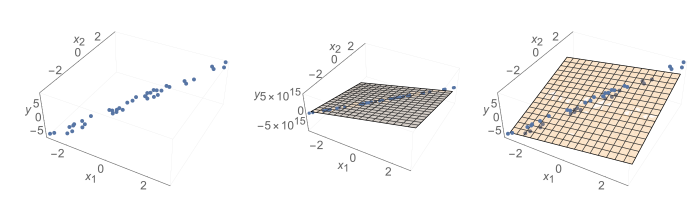
\includegraphics[width=120mm,scale=0.5]{images/regression_images/Regularizer_Multiple_Solutions.png}
        
            \caption*{There are many \textbf{planes} that can go through this line: multiple equally good solutions!}
        \end{figure}
        
        \begin{figure}[H]
        \centering
            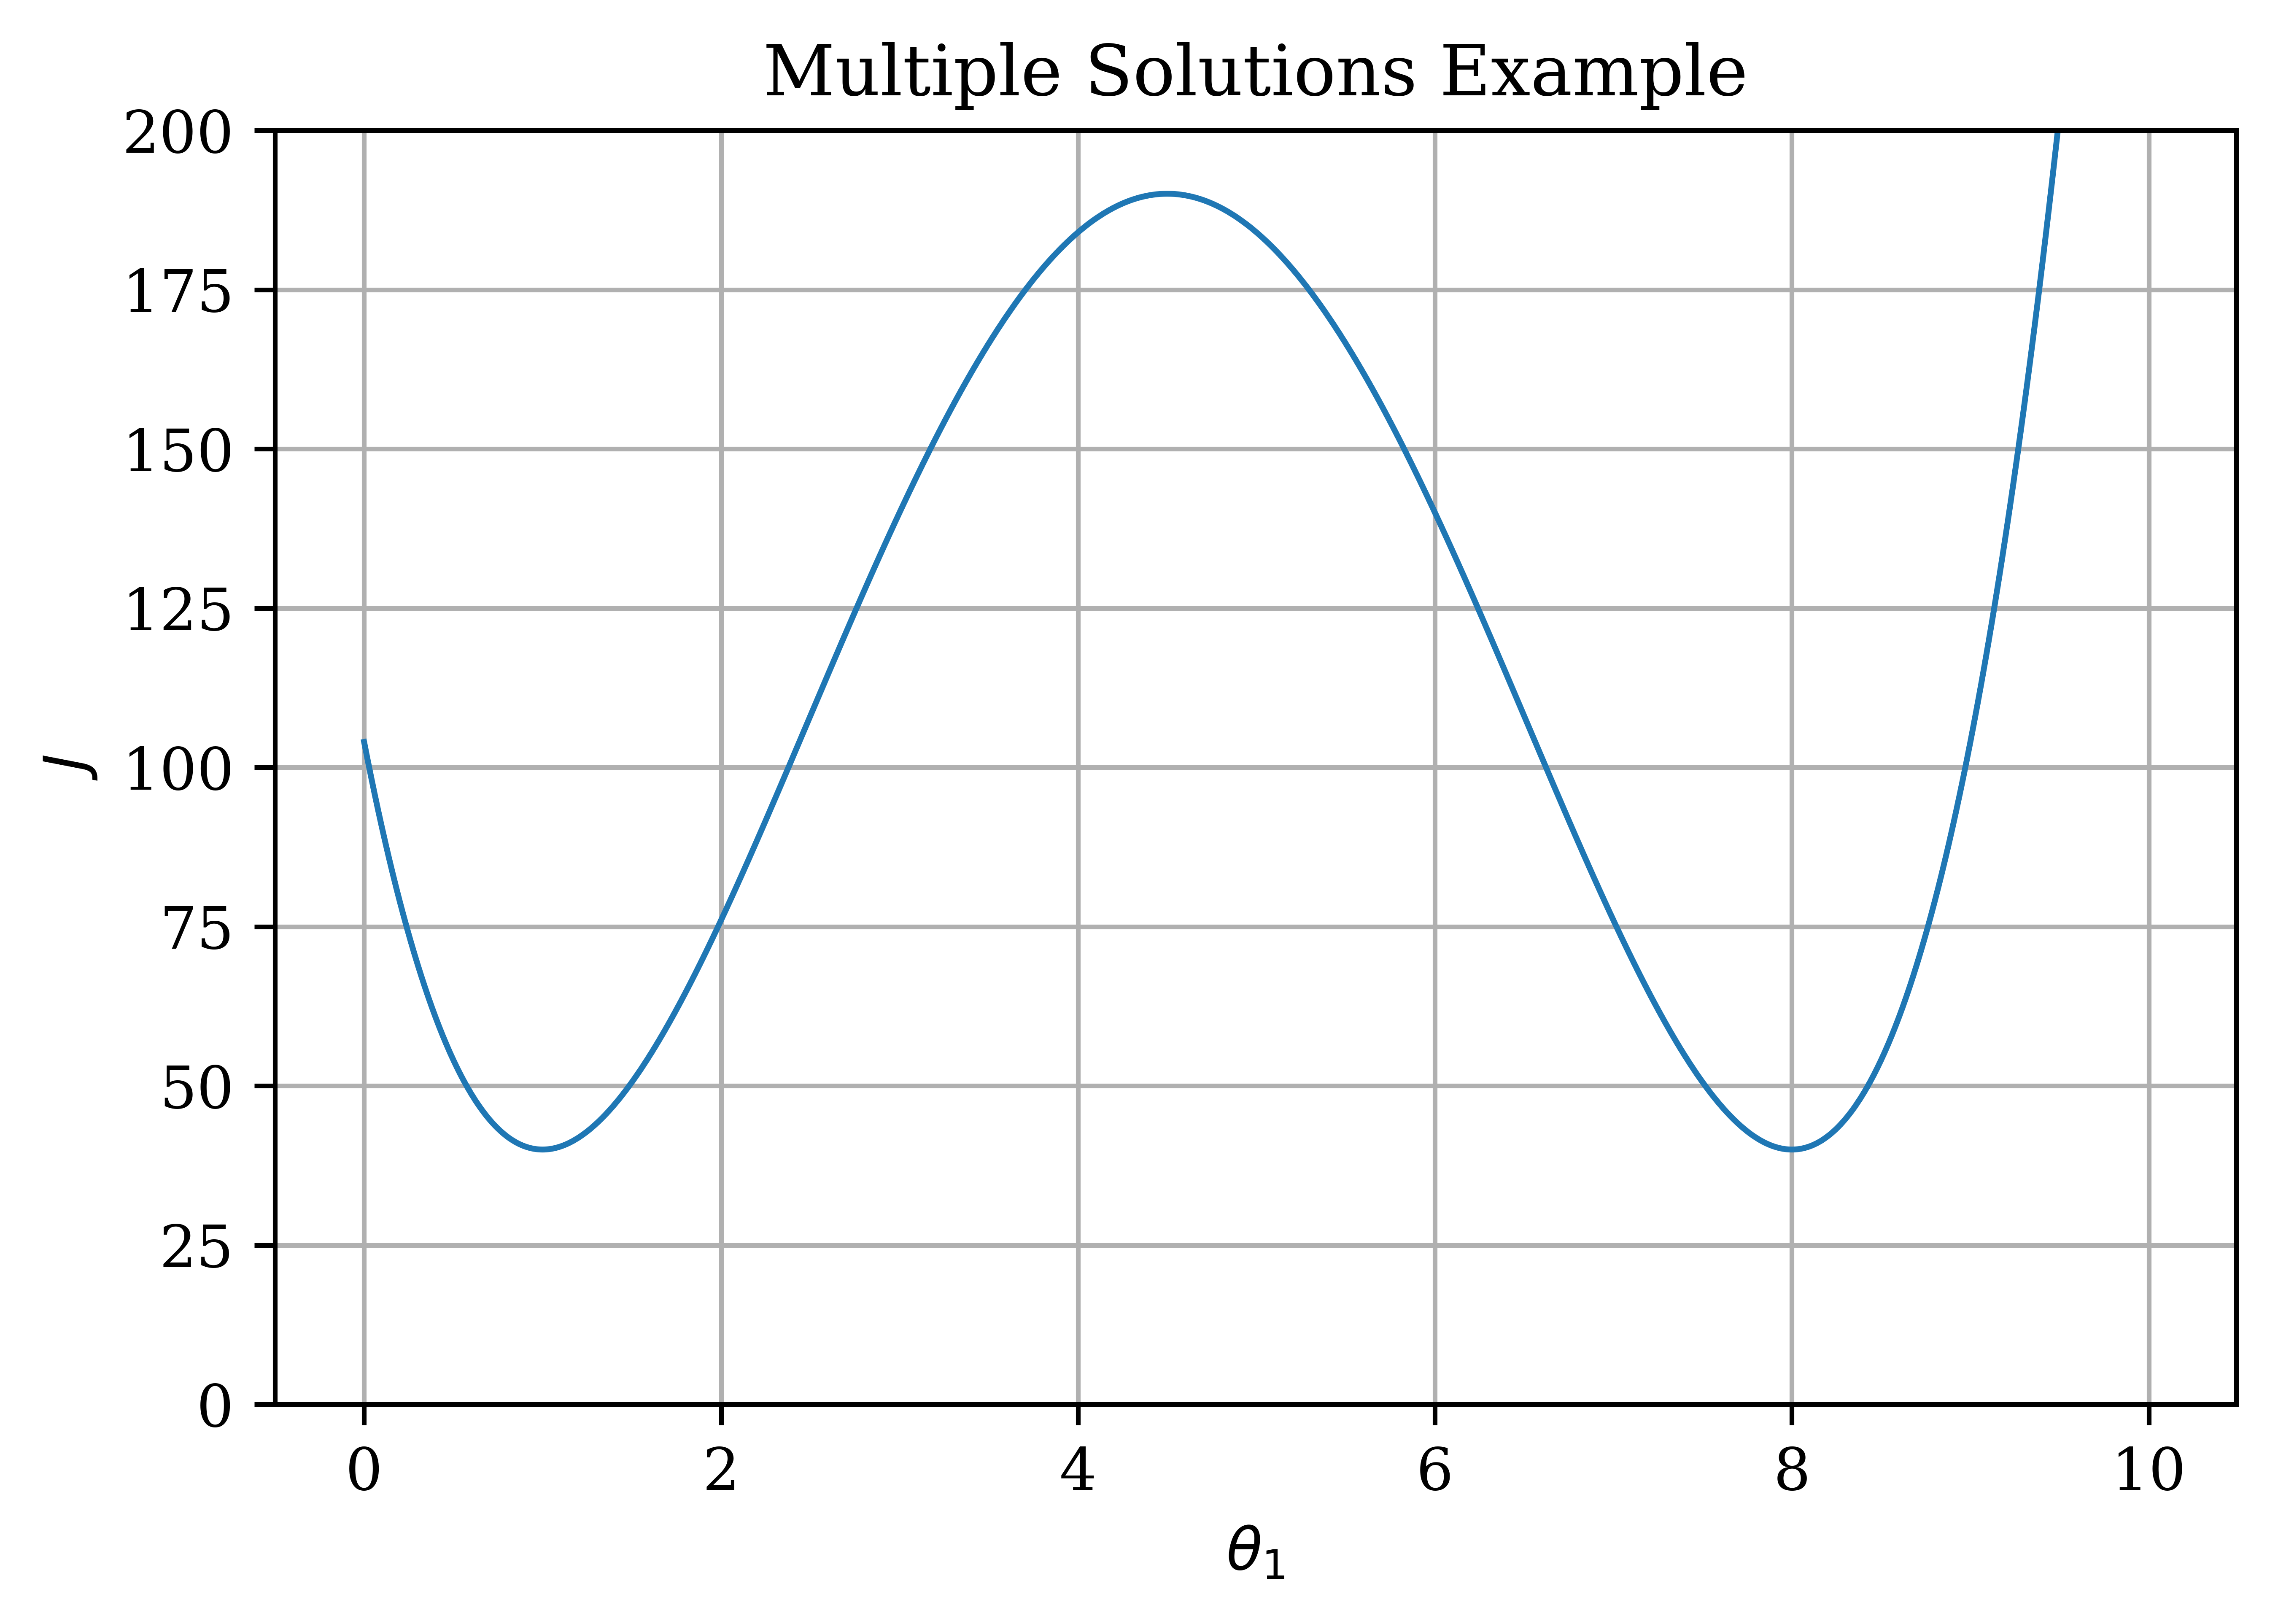
\includegraphics[width=70mm,scale=0.5]{images/regression_images/Regression_Multiple_Solutions_Example.png}
        
            \caption*{This compares different hypotheses ($\theta_1$) and sees how well they perform ($J$): two are equally good!}
        \end{figure}
        
        Either way, we can pick a solution based on lowest $\theta$ \textbf{magnitude}!
        
    \subsection{A Math Perspective: Unique Solutions}    
        
        We can also view this problem more \textbf{mathematically}.
        
        Let's look at our \textbf{analytical} solution:
        
        \begin{equation}
            \theta = 
                \inv{  \left(  XX^T  \right)  }   X Y^T
        \end{equation}
        
        This solution only works if $\inv{  \left(  XX^T  \right)  }$ is \textbf{valid}. But we have a problem: \textbf{not all matrices} have \textbf{inverses}. 
        
        If $XX^T$ has a \textbf{determinant} of \textbf{zero}, then we cannot find an inverse. 
        \note{This is an important idea in linear algebra! If you don't know what this means, here's a 
        \href{https://www.youtube.com/watch?v=uQhTuRlWMxw&list=PL0-GT3co4r2y2YErbmuJw2L5tW4Ew2O5B&index=8}{great video}.
        }
        
        Without an inverse, we have \textbf{no unique solution}! This is a problem.
        
        This is one thing our \textbf{regularizer} $R(\Theta)$ helps us solve: we'll see that our \textbf{new solution} will not have this problem! 
        
        The reason will be clear in the \textbf{algebra}, but it's \textbf{equivalent} to the reason we discussed the above: we take the best \textbf{models} that are all \textbf{equally good}, and pick the one with \textbf{lowest magnitude}.\\
        
        \begin{concept}
            \vocab{Ridge Regression} helps \purp{improve} our model by
            
            \begin{itemize}
                \item Making our model more \purp{general} and resistant to \gren{overfitting}
                \item Making sure \gren{solutions} are \purp{unique}
                \item Keeping our matrix $XX^T$ \purp{invertible}, so we can find a \gren{solution}.
            \end{itemize}
        \end{concept}
        
    \subsection{Lambda, a.k.a. $\lambda$}
    
        We now have a term that can help us choose a more \textbf{general} hypothesis. One important question is, \textbf{how general} do we want it to be?
        
        The more general we make our model, the \textbf{less specific} to our current data it is. This may seem like a good thing, but too much can make our model \textbf{worse}!
        
        If $\lambda$ is \textbf{too large}, then your model will stay \textbf{very close} to $\norm{\theta}=0$. This probably isn't a good solution for most cases.
        
        %Diagram of flat slope
        
        But if it's \textbf{too small}, then it \textbf{won't} have enough of an \textbf{effect}. So, we need to be able to adjust how \textbf{much} we're regularizing.
        
        To do this, we will \textbf{scale} our regularizer by a \textbf{constant} factor, $\lambda$.\\
        
        \begin{definition}
            \vocab{Lambda}, or \vocab{$\lambda$}, is the constant we \gren{scale} our \purp{regularizer} by.
            
            It represents \gren{how strongly} we want to regularize: how much we prioritize \purp{general} understanding over \purp{specific} understanding.
        \end{definition}
    
    
        %Follow up with a section about hyperparameter tuning
    
    \subsection{Our new objective function}
    
        Now that we have our regularizer,
        
        \begin{equation}
            R(\Theta) = \lambda \norm{\theta}^2
        \end{equation}
        
        We can add it to our objective function:\\
        
        \begin{kequation}
            The \vocab{objective function} for \vocab{ridge regression} is given as 
            
            \begin{equation*}
                J(\theta) = 
                            \frac{1}{n}  \sum_{i=1}^n 
                            \left( 
                                \underbrace{
                                    \red{(\theta^T \ex{x}{i}  
                                    + \theta_0)}
                                }_{guess}
                                - \underbrace{
                                    \blu{\ex{y}{i}} 
                                }_{answer}
                            \right)^2 
                            + 
                            \underbrace{
                                \pur{ \lambda \norm{\theta}^2 }
                            }_{Regularizer}
            \end{equation*}
        \end{kequation}
        
        This is the form we will \textbf{solve}.
    
    \subsection{Matrix Form Ridge Regression}
        
        Just like before, we'll switch from a \textbf{sum} to a \textbf{matrix} in order to solve this problem.
        
        Creating an \textbf{equation} for both $\theta$ and $\theta_0$ is, frankly, \textbf{annoying} to \textbf{derive}. \textbf{Instead}, we'll cheat a little, and keep $\theta_0$ in and create our \textbf{matrix-form} objective function:
        
        \begin{equation}
            J = \frac{1}{n}
                \blu{
                    \left( \Xt \theta  - \Yt  \right)^T
                    \left( \Xt \theta  - \Yt  \right) 
                }
                + 
                \pur{\lambda 
                    \left( \theta^T \theta    \right)
                }
        \end{equation}
        
        Our work begins. Let's take the \textbf{gradient}: what we want to set to zero.
        
        \begin{equation}
            \nabla_\theta J = 
                \frac{2}{n} 
                \blu{
                    \Xt^T
                    \left( \red{ \Xt \theta  - \Yt } \right) 
                }
                +
                \pur{ 2 \lambda \theta}
            =0
        \end{equation}
        
        We do some algebra and \textbf{solve} as we do in the \textbf{official notes}:\\
        
        \begin{kequation}
            The \vocab{solution} for \vocab{ridge regression optimization} is 
            
            \begin{equation*}
                \theta = 
                \inv{ 
                    \left(  \Xt^T\Xt + n \lambda I \right)  
                }
                \Xt^T  \Yt
            \end{equation*}
            
            Or, in our \pur{original} notation,
            
            \begin{equation*}
                \theta = 
                \inv{ 
                    \left(  XX^T + n \lambda I \right)  
                }
                XY^T
            \end{equation*}
            
        \end{kequation}
        
    \subsection{Our new term, $n \lambda I$}
    
        So, we already established that \textbf{regularization} helps us create more \textbf{general} hypotheses that are lower in magnitude.
        
        But, how does this \textbf{mathematically} solve our invertibility problem?
        
        \begin{equation}
            \theta = 
                \inv{ 
                    \left(  XX^T + \pur{ n \lambda I } \right)  
                }
                XY^T
        \end{equation}
        
        This term, $n \lambda I$, is added to the matrix we want to invert. Let's see what this matrix looks like. We'll use a $(3 \times 3)$ example:
        \note{$I$ is the \textbf{identity matrix} in our notation.}
        
        \begin{equation}
            n \lambda I 
            = 
            n \lambda 
            \begin{bmatrix}
                1 & 0 & 0\\
                0 & 1 & 0\\
                0 & 0 & 1\\
            \end{bmatrix}
            =
            n
            \begin{bmatrix}
                \lambda & 0         & 0        \\
                0         & \lambda & 0        \\
                0         & 0         & \lambda\\
            \end{bmatrix}
        \end{equation}
        
        This visual, having a "\textbf{ridge}" of $\lambda$s along the diagonal, is why we call it \textbf{ridge regression}.
        
    \subsection{Invertibility}
        
        This term $n\lambda I$ \textbf{shifts} the values of $XX^T$ so that we \textbf{avoid} having a \textbf{determinant of zero}.
        
        Since the \textbf{determinant is nonzero}, we don't have to worry about an \textbf{uninvertible matrix}: we now have a \textbf{unique} inverse, and thus a \textbf{unique} solution.\\
        
        \begin{concept}
            \vocab{Ridge Regression} solves the problem of \vocab{matrix invertibility} (non-unique solutions) by adding a term \purp{$n \lambda I$}, our \gren{ridge} of diagonals.
            
            This turns the inverse $\inv{(XX^T)}$ into 
            
            \begin{equation*}
                \inv{(XX^T + n \lambda I)}
            \end{equation*}
            
            Which can prevent a \purp{determinant} of zero in our solution, given $\lambda>0$.
        \end{concept}
        
        
        
    
\pagebreak
%%%%%%%%%%%%%%%%%%%%%%%%%%%%%%%%%%%%%%%%%%%%%%%%%%%%%%%%%%%%%%%%%%%%%%%%%%%%%%%%%%%%%%%%%%%
        
\section{Evaluating Learning Algorithms}

    Now, we have successfully developed an \textbf{algorithm} for \textbf{learning} from our data. But, did our algorithm make a \textbf{good} hypothesis? How do we do \textbf{better}?
    
    \subsection{What $\lambda$ should we choose?}
    
        There's something we ignored earlier: how do we pick the \textbf{best} value of $\lambda$? We didn't go into detail, but that value of $\lambda$ will affect our algorithm's \textbf{performance}.
        
        This $\lambda$ adjusts exactly how we \textbf{learn}: how much more do we learn \textbf{specifically}, versus \textbf{generally}?
    
        We mentioned that different $\lambda$ values have different \textbf{tradeoffs}, so we need to figure out which $\lambda$ value is best for our problem.
        
        We'll need to \textbf{optimize} our $\lambda$ value! Let's figure out how to go about that.
        
    \subsection{Tradeoffs: Estimation Error}
    
        High and low $\lambda$ values have benefits and drawbacks. These tradeoffs can be loosely divided into \textbf{two categories}.
        
        When we generalize, we're trying to avoid \vocab{estimation error}: we incorrectly guess the overall distribution we're trying to fit. We \textbf{estimate} poorly if we \textbf{generalize} poorly.\\
        
        \begin{definition}
            \vocab{Estimation error} is the error that results from poorly \gren{estimating} the \purp{solution} we're trying to find. 
            
            This can be caused by \gren{overfitting}, getting a bad (\purp{unrepresentative}) sample, or not having enough \gren{data} to come to conclusion.
        \end{definition}
        
        \miniex Let's try a regression problem, but we'll use only 4 points to make our plot.
        
        \begin{figure}[H]

            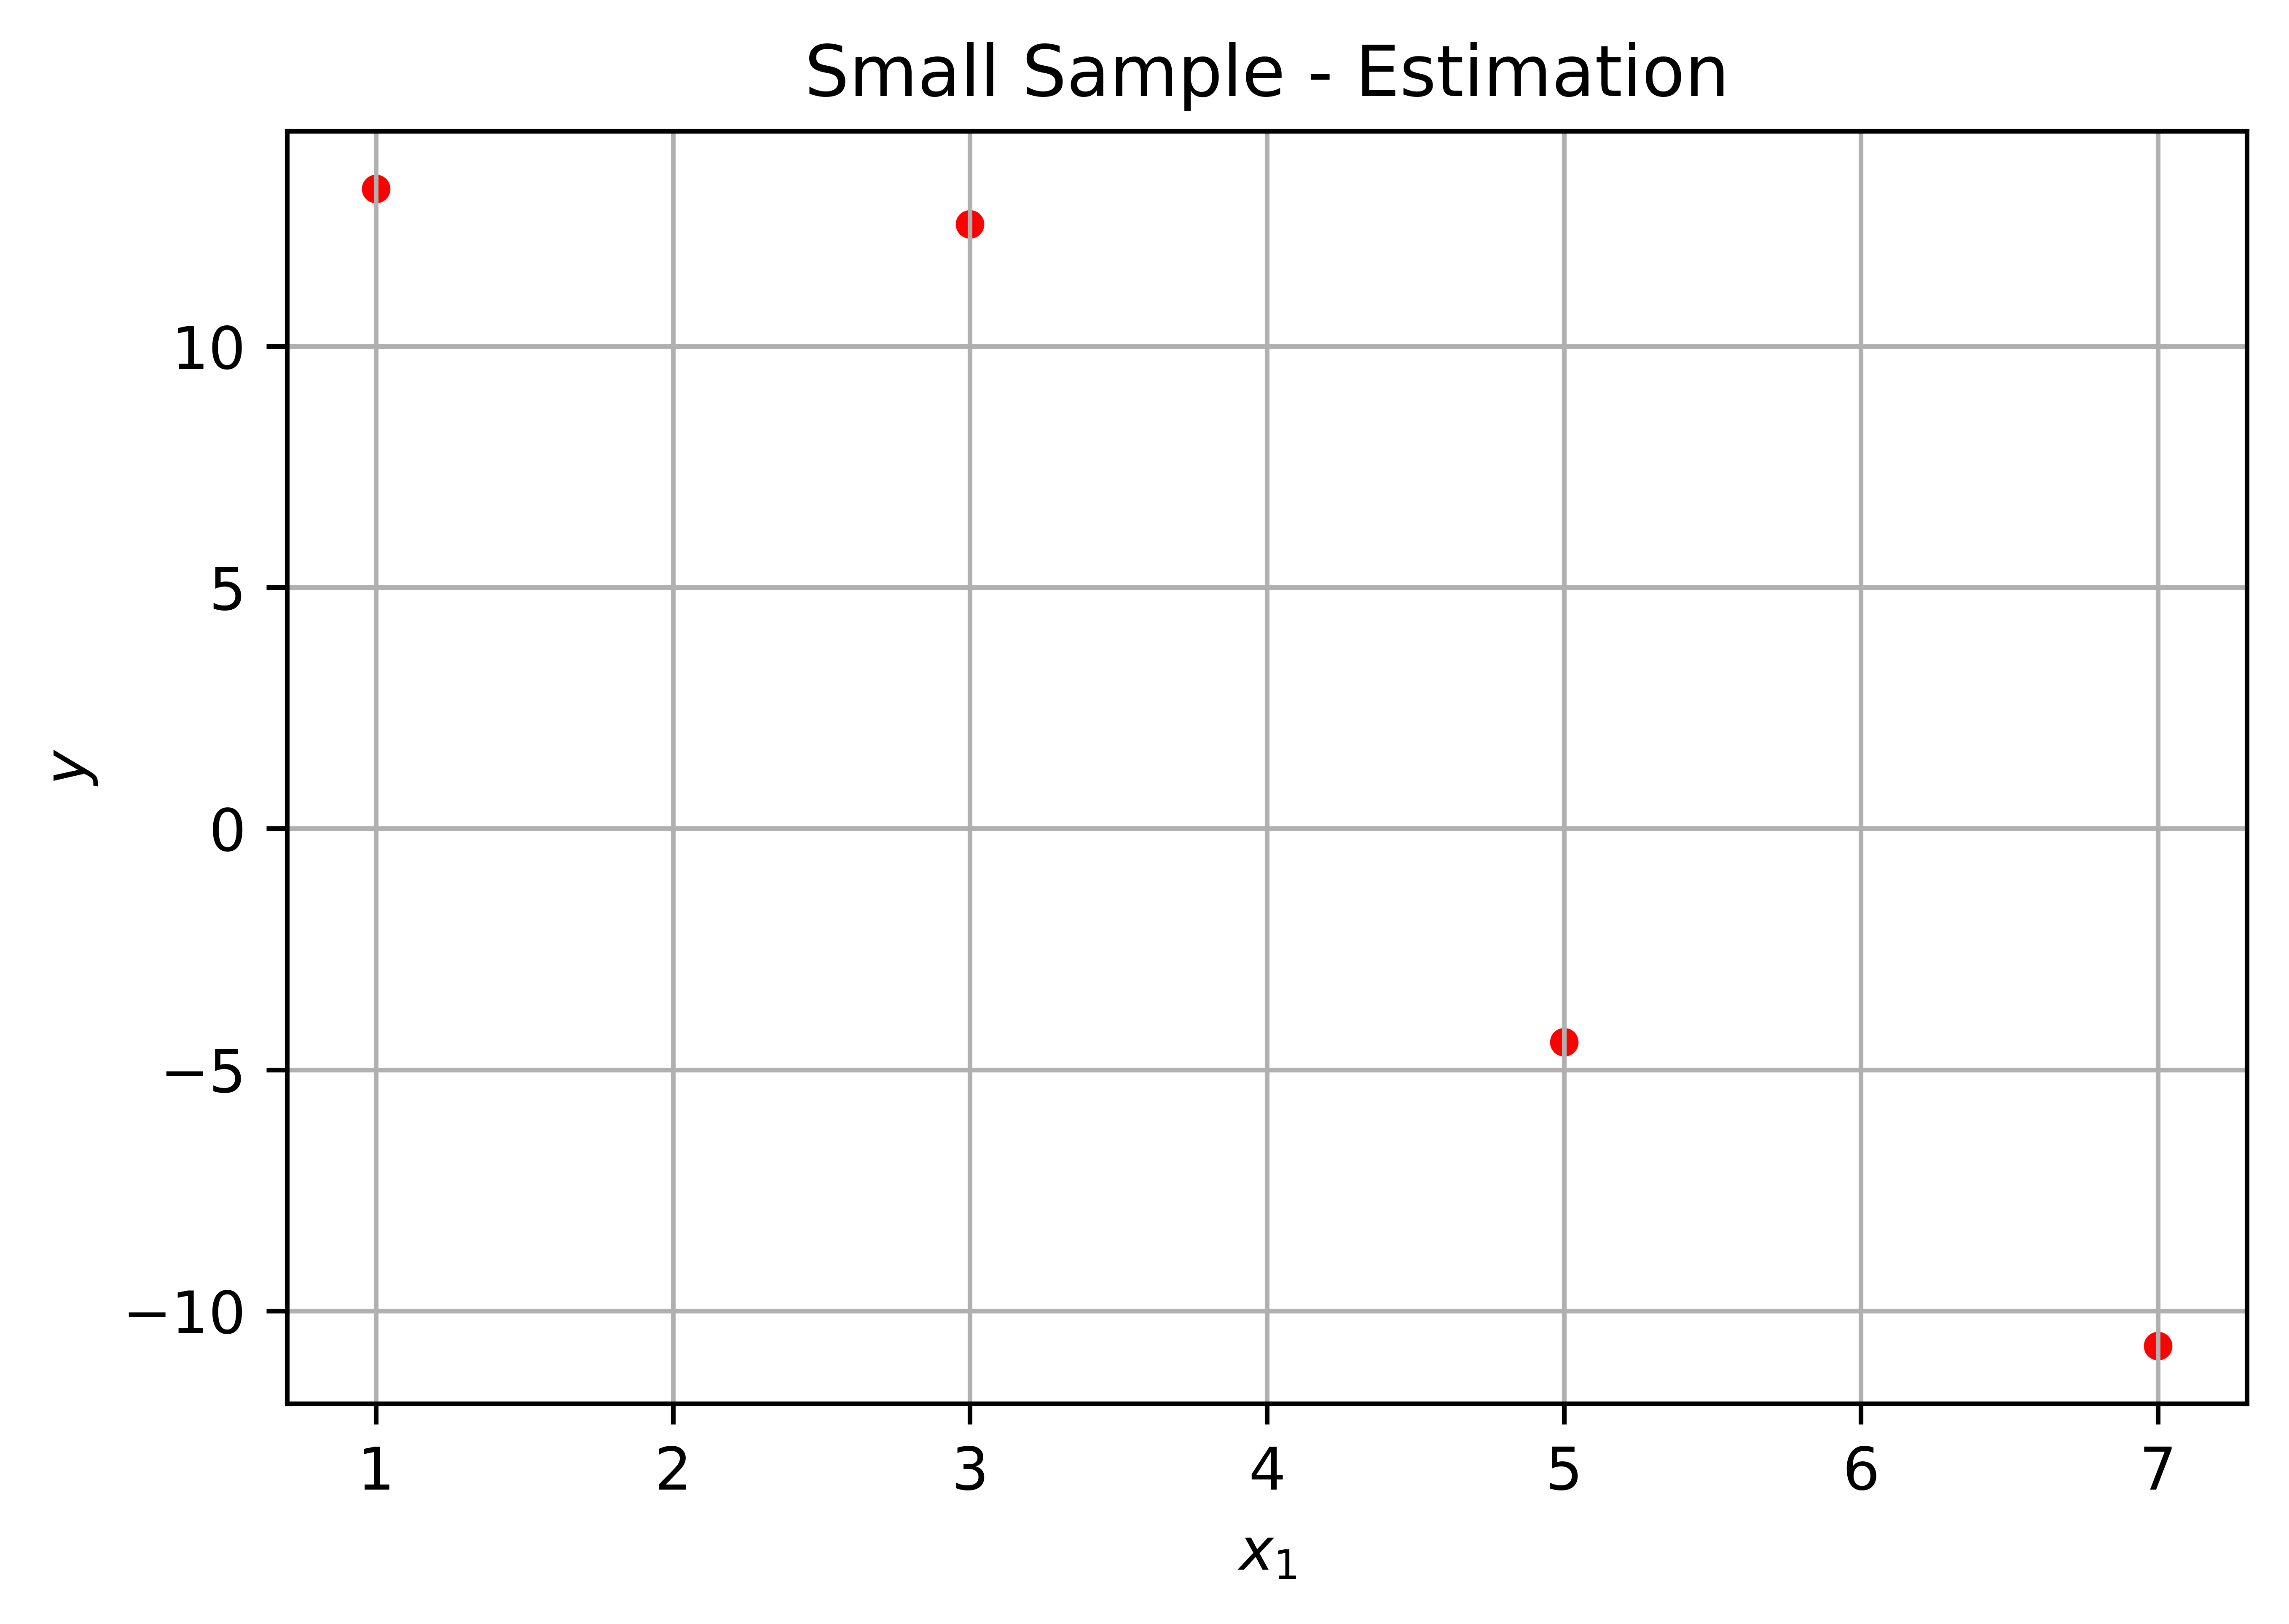
\includegraphics[width=70mm,scale=0.5]{images/regression_images/Estimation_Limited_Sample.png}

            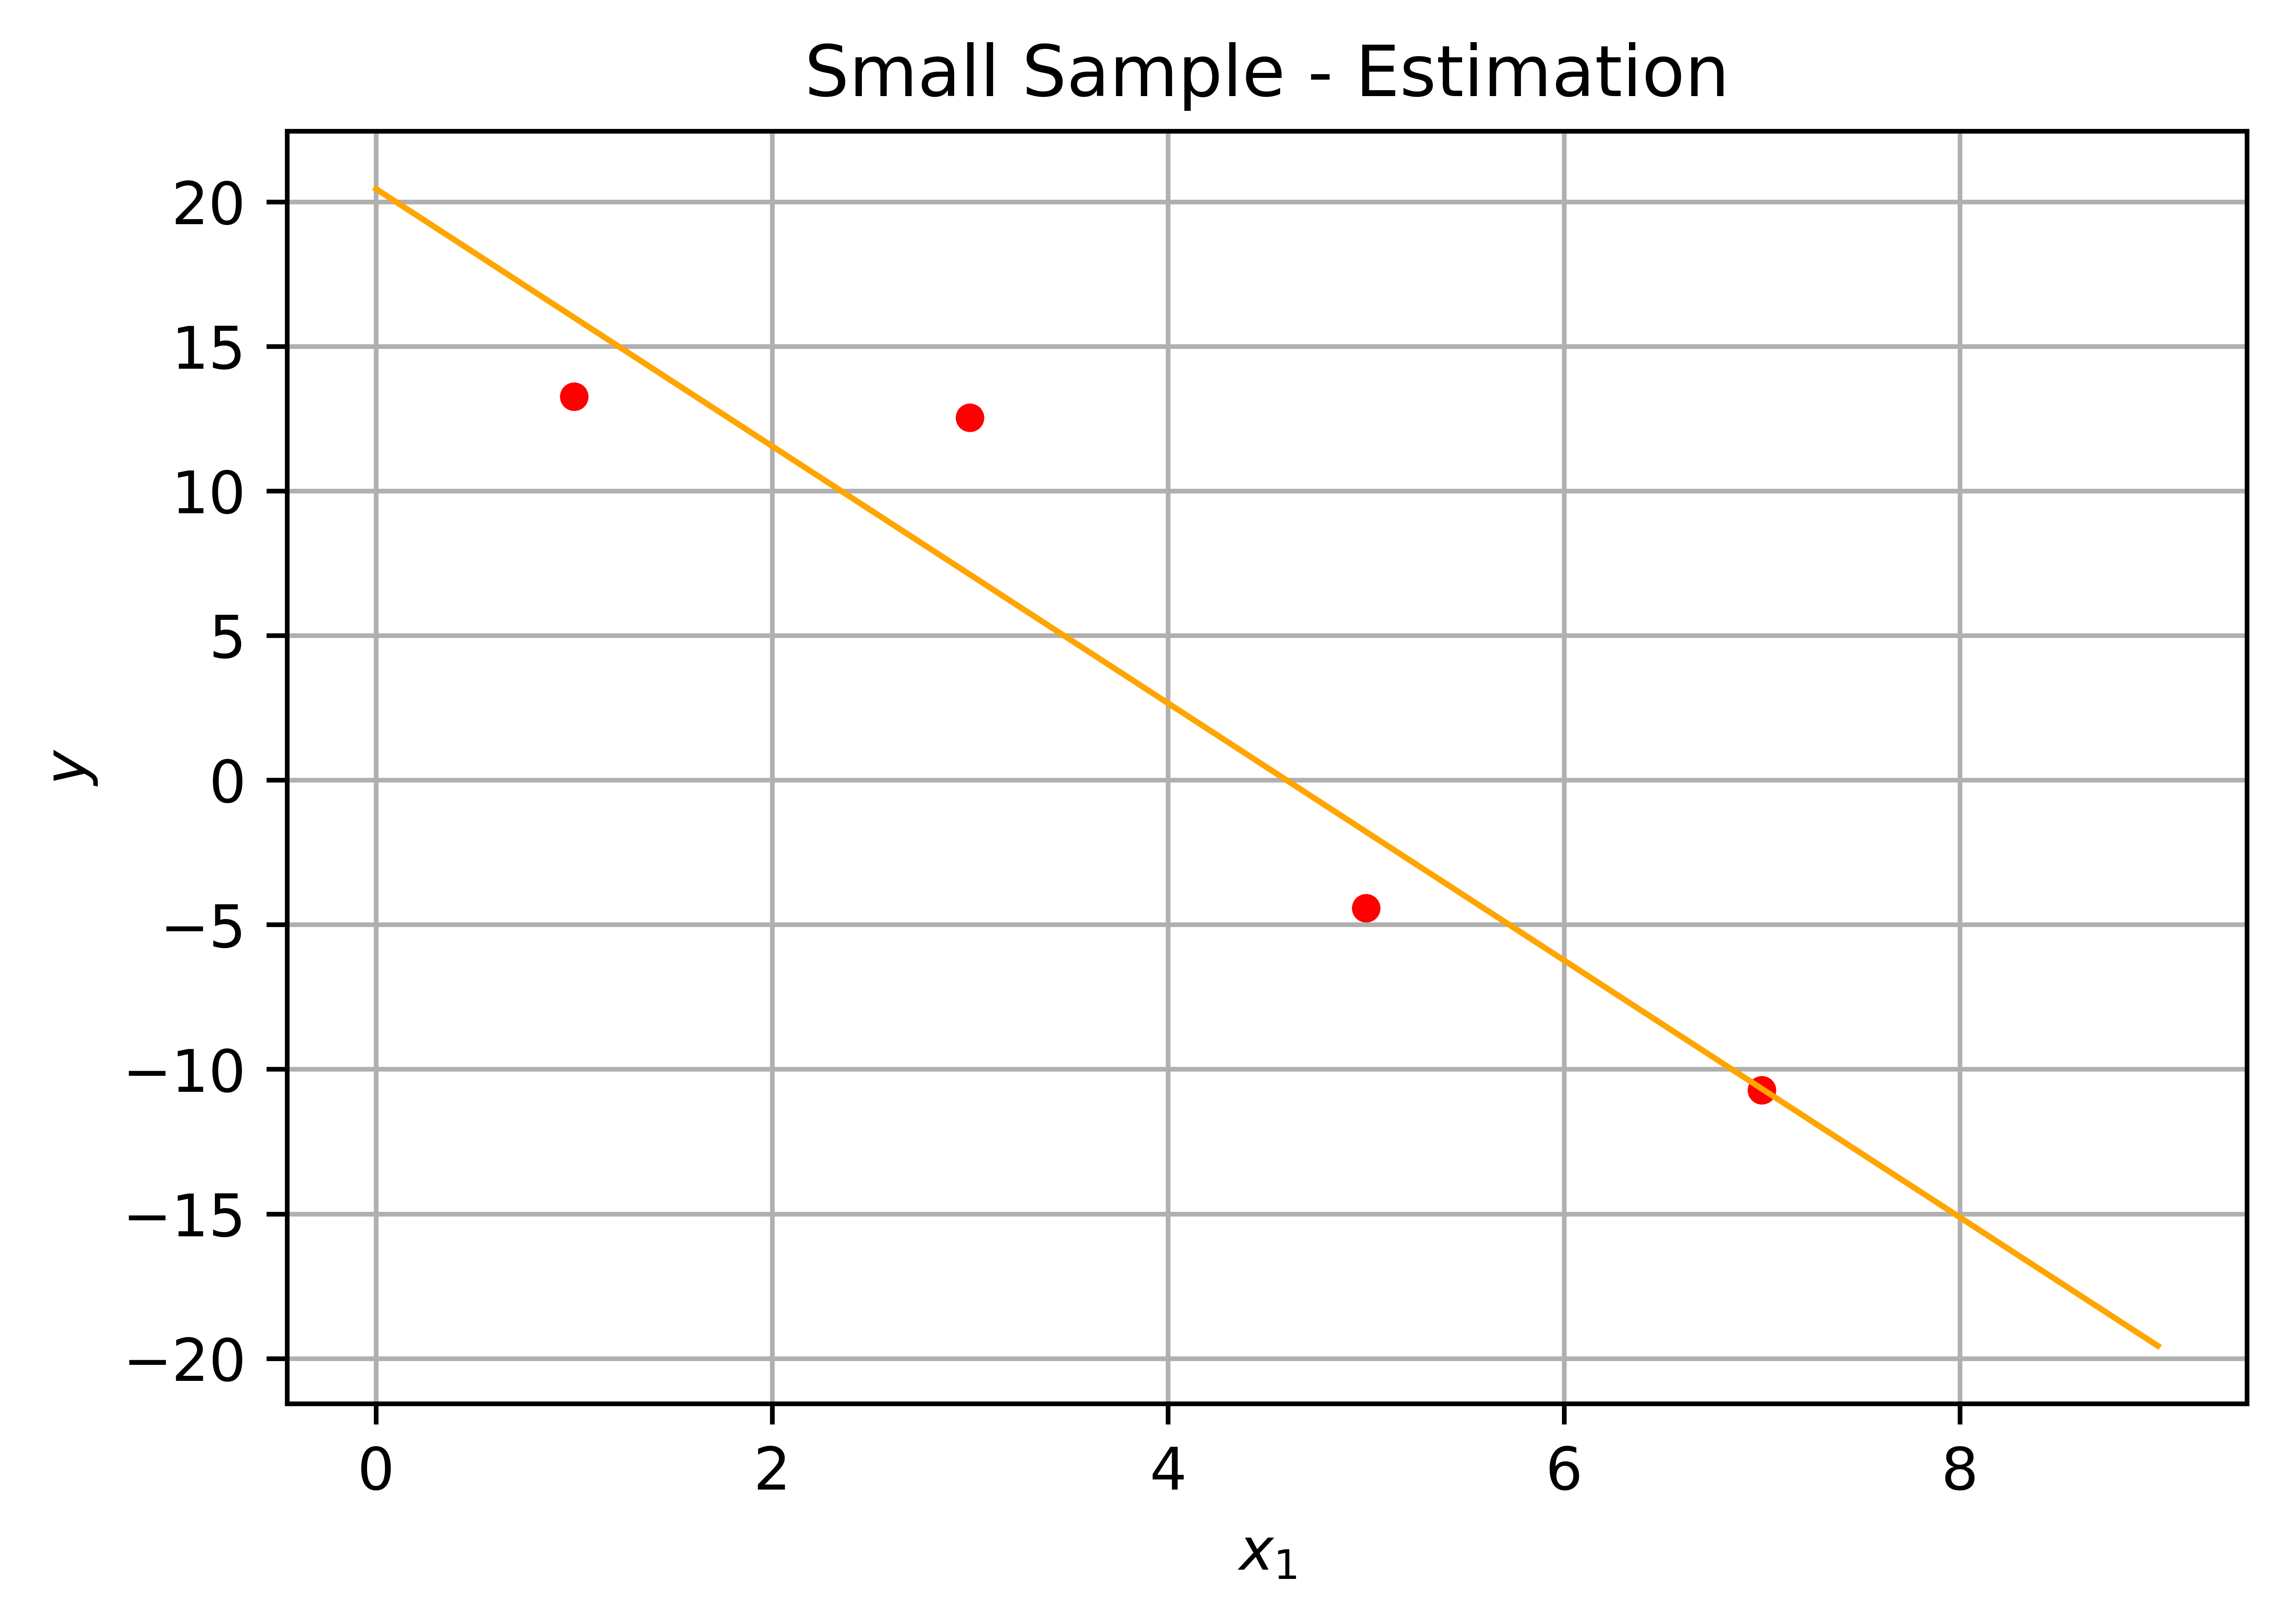
\includegraphics[width=70mm,scale=0.5]{images/regression_images/Estimation_Limited_Sample_Regression.png}
        
            \caption*{This is the regression solution we get based on our small dataset.}
        \end{figure}
        
        We might be suspicious. One way to reduce \textbf{estimation error} is to increase our number of data points (though this isn't always an option, or sufficient!)
        
        \begin{figure}[H]

                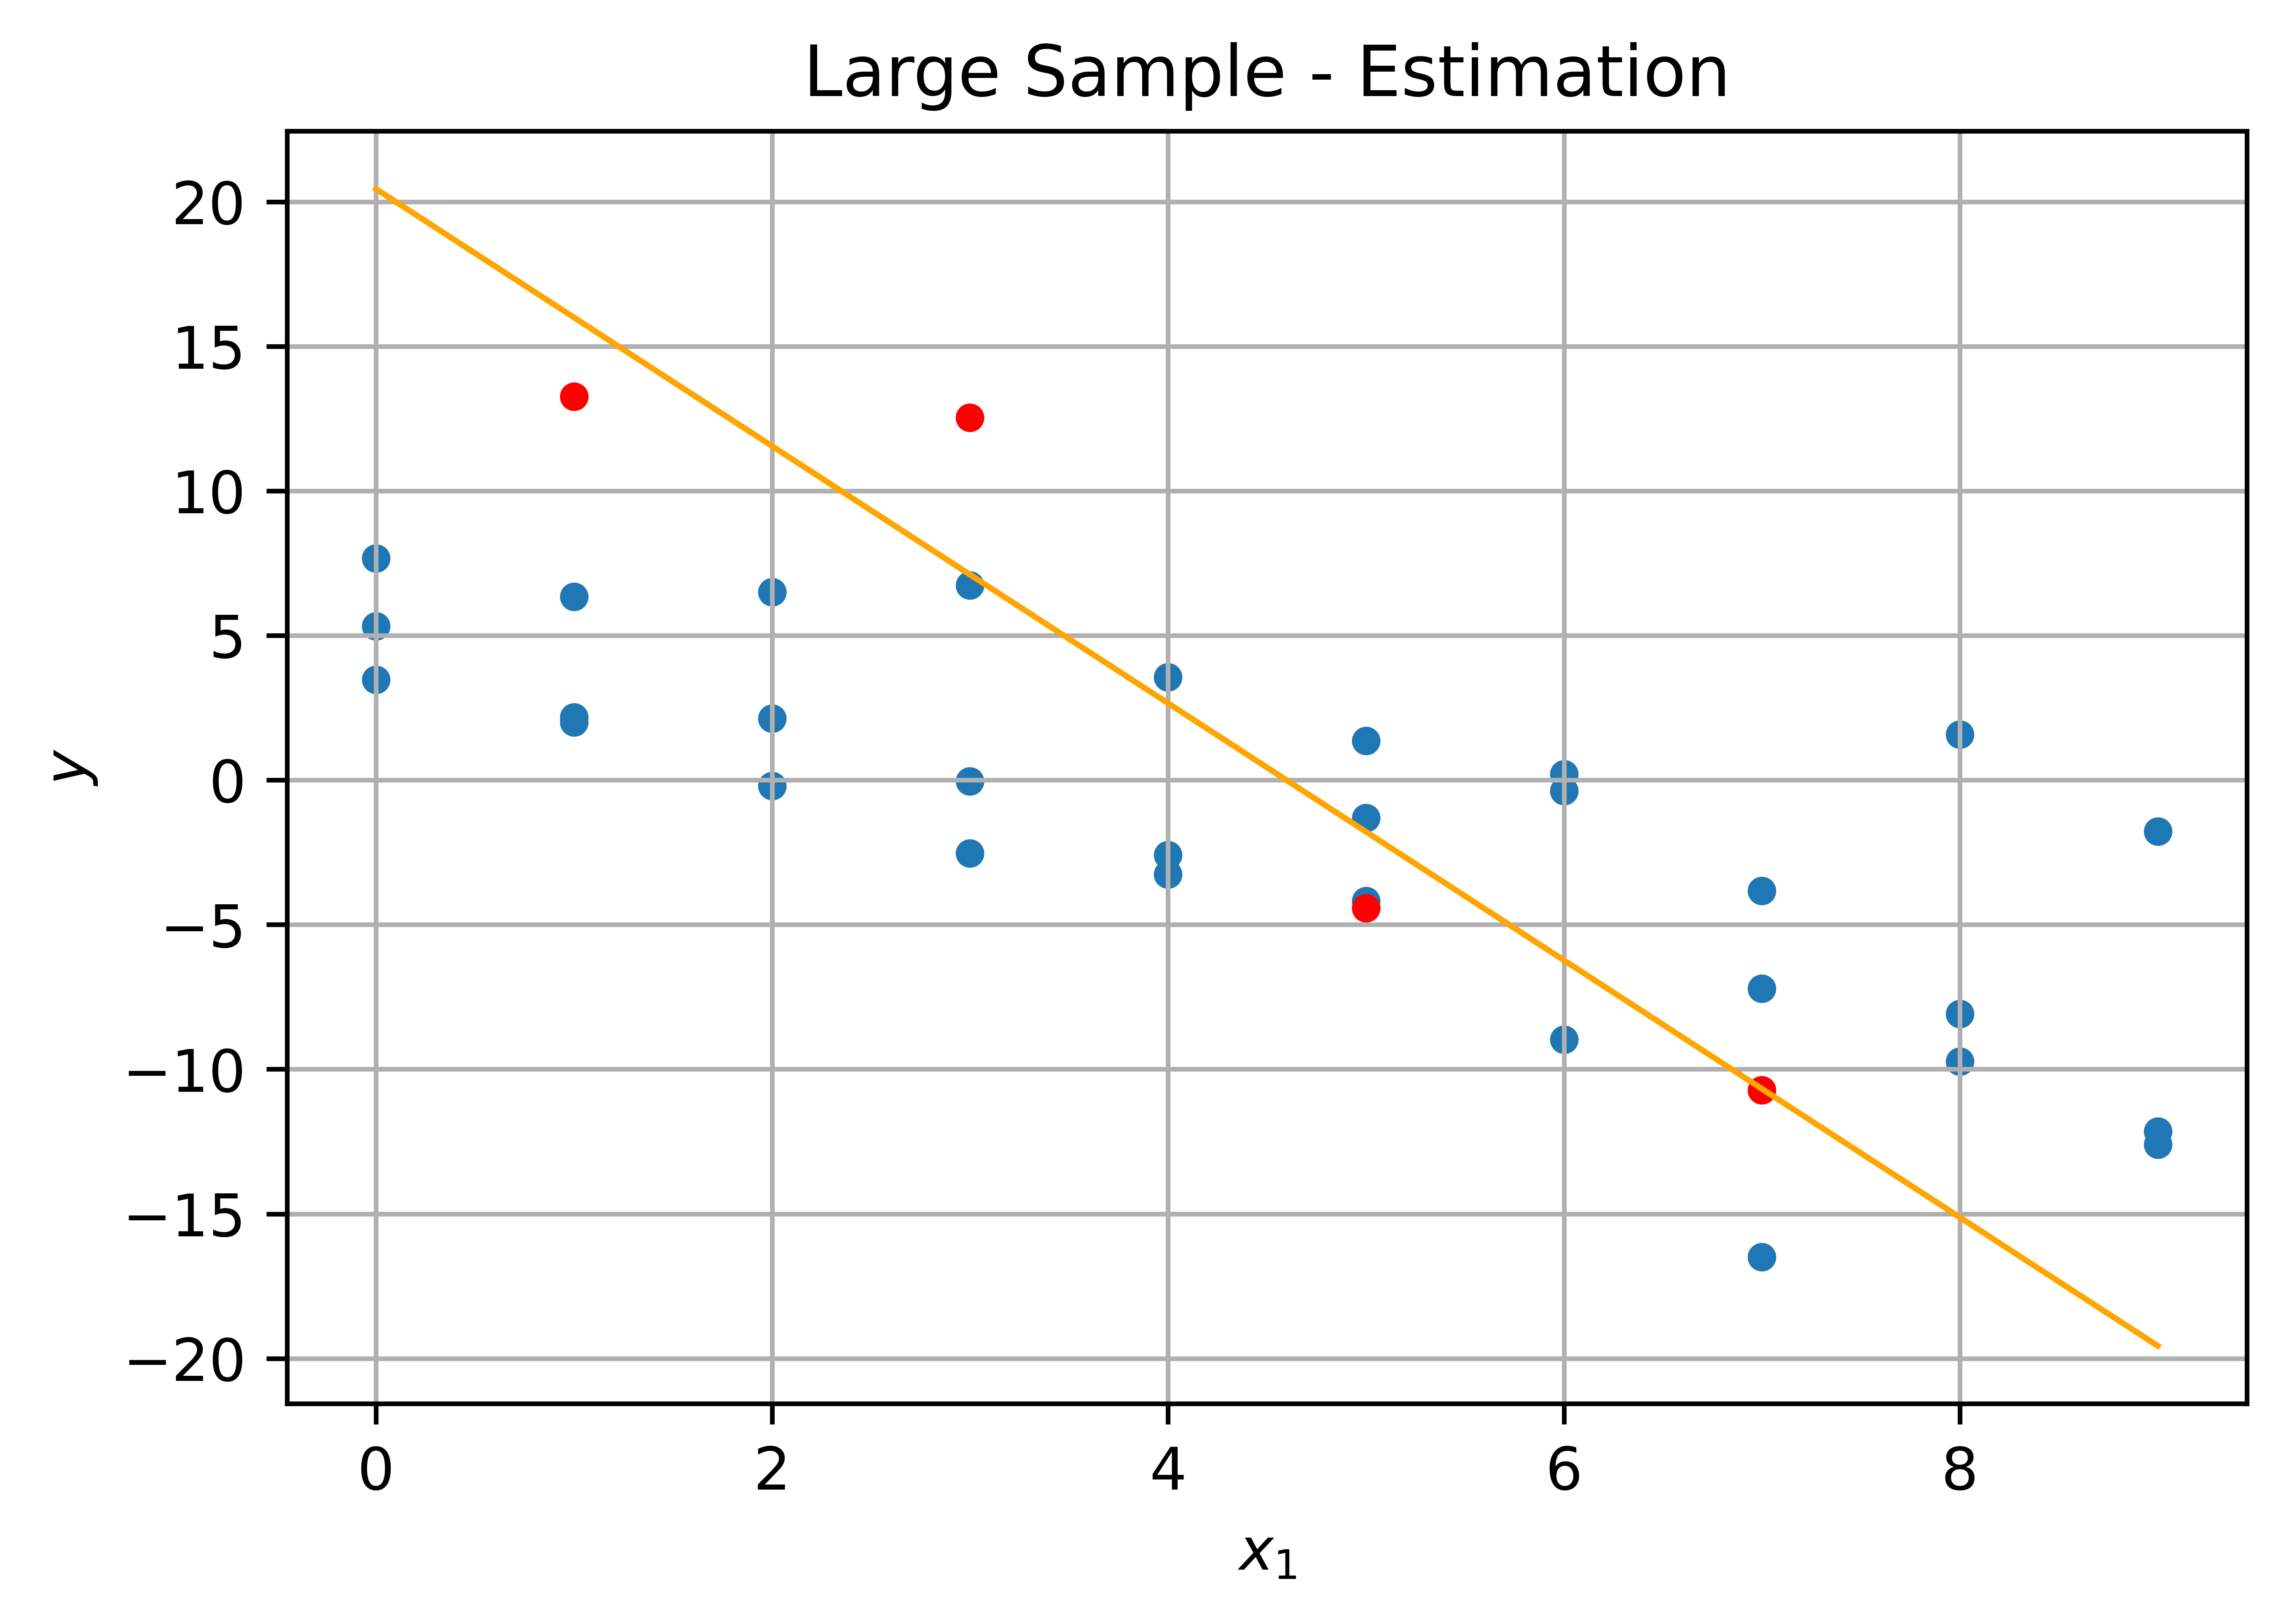
\includegraphics[width=70mm,scale=0.5]{images/regression_images/Estimation_Full_Sample.png}
                
                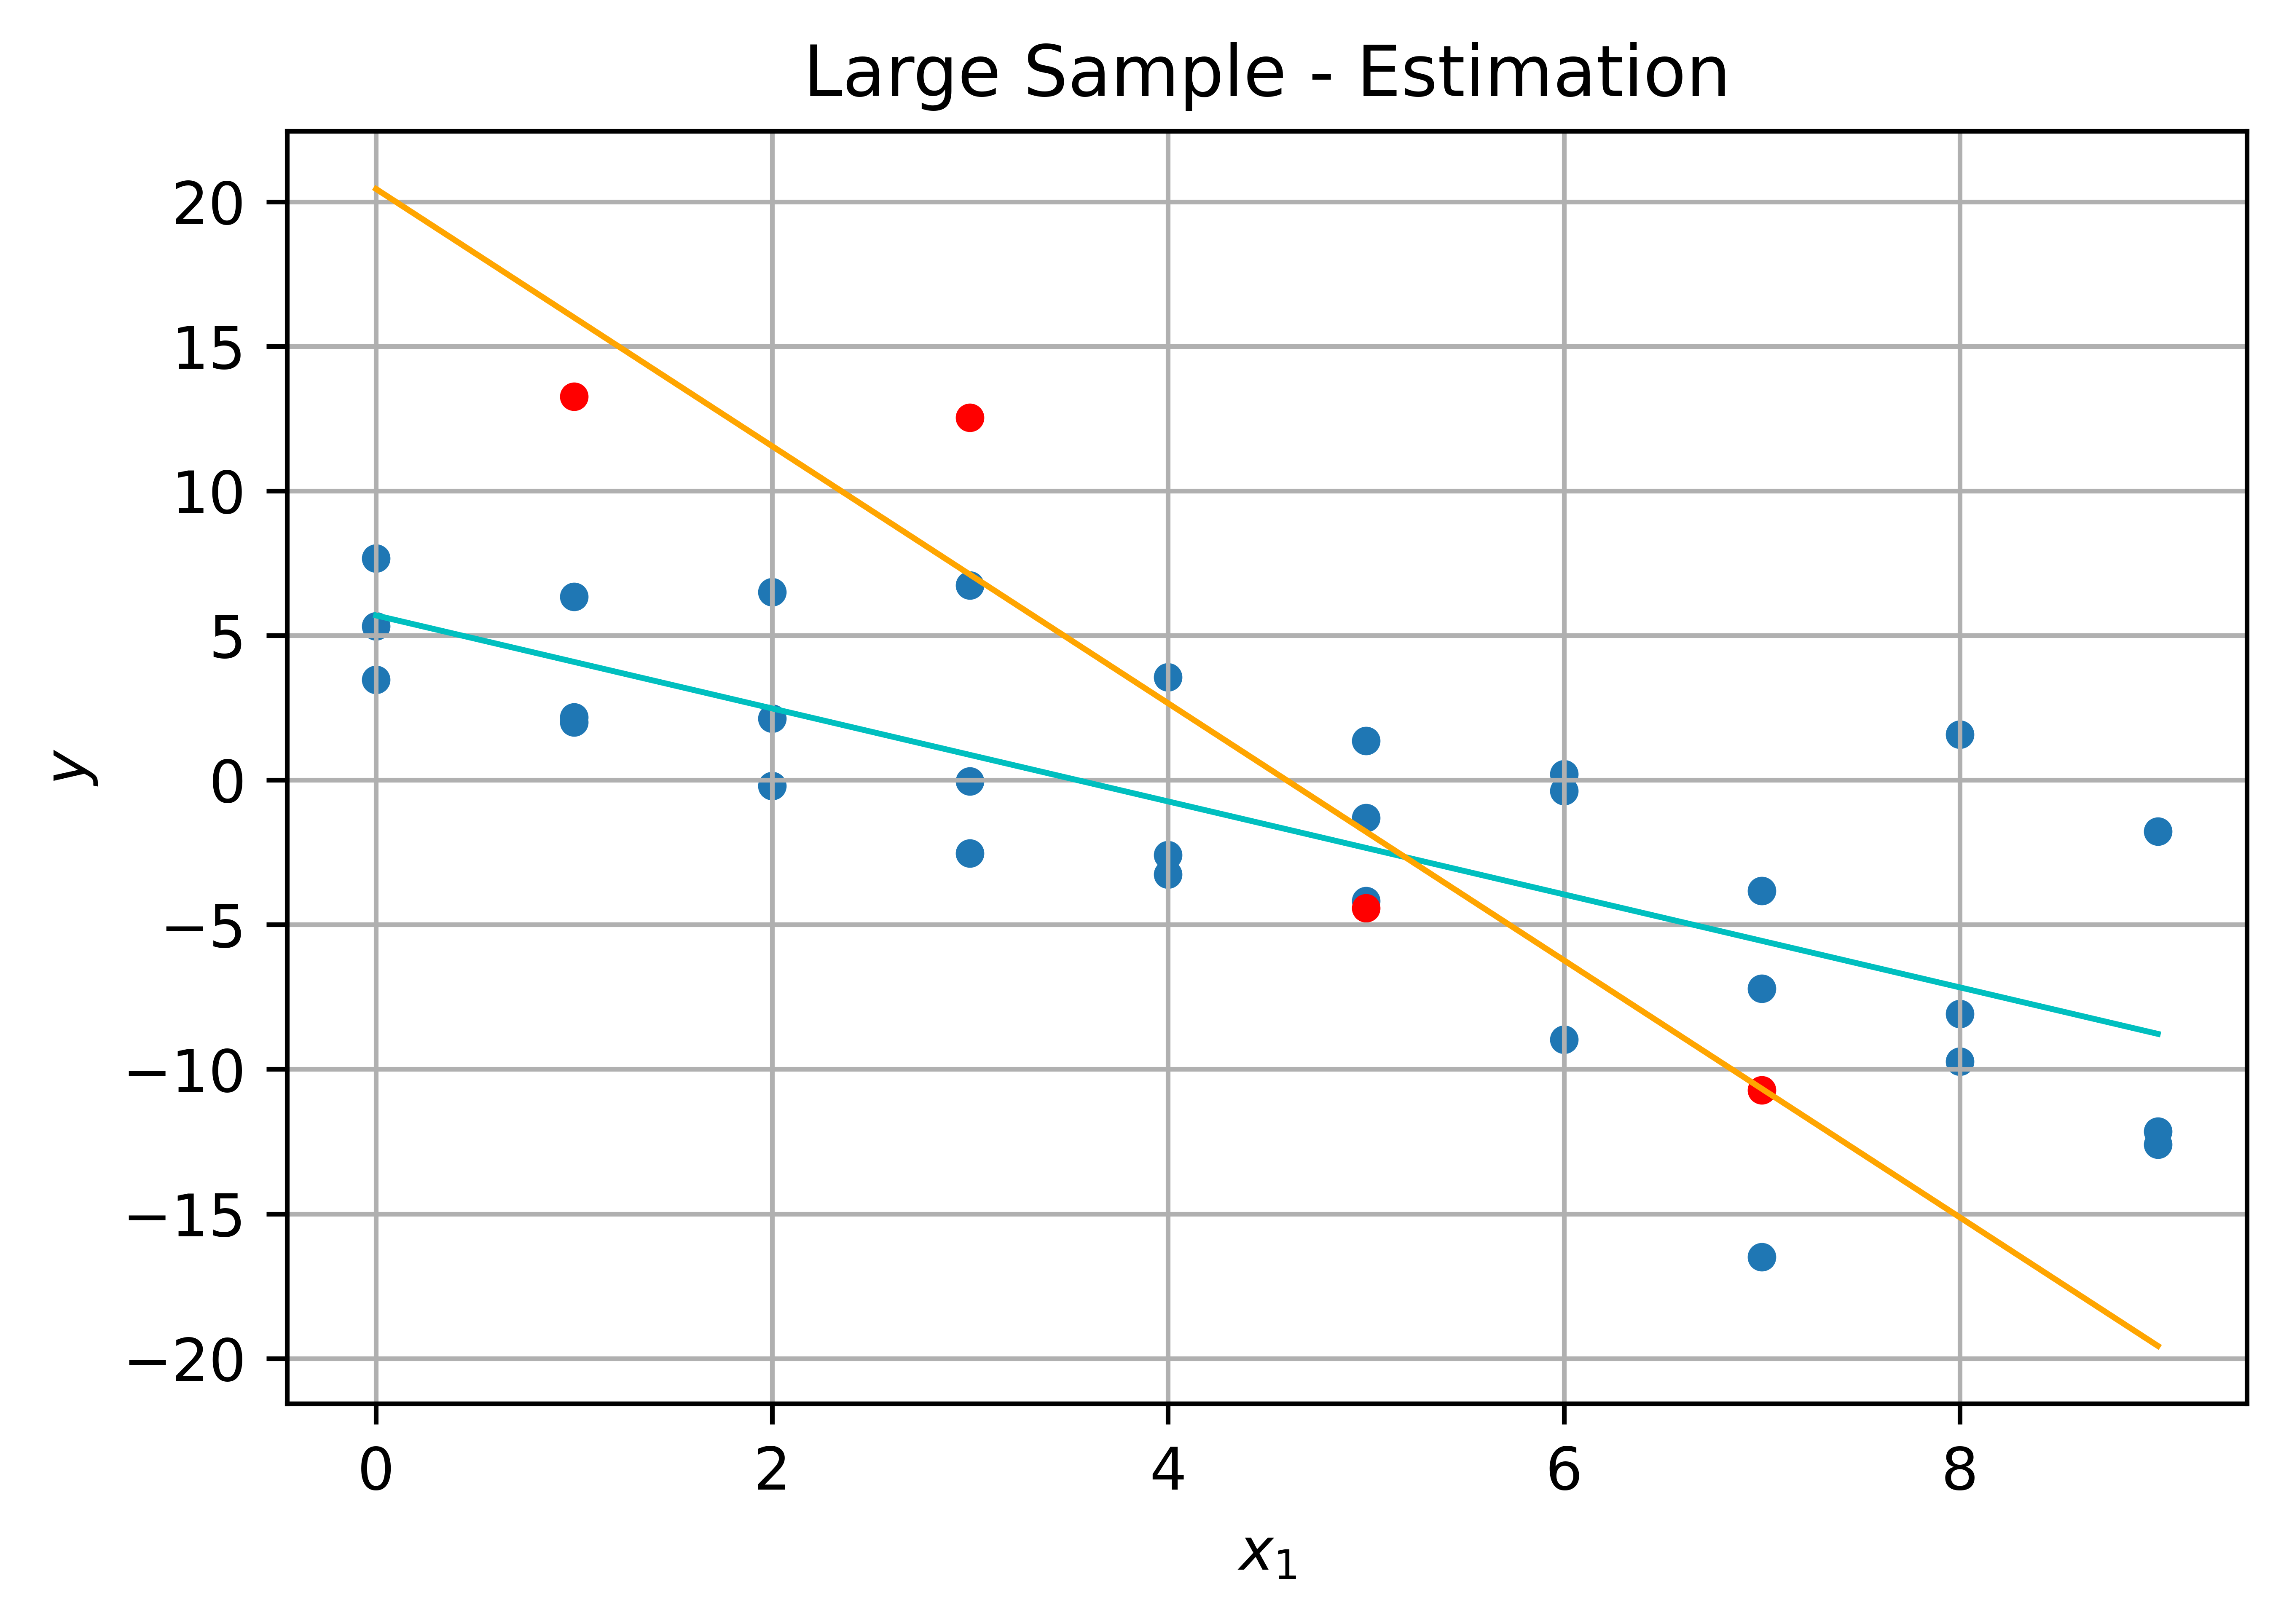
\includegraphics[width=70mm,scale=0.5]{images/regression_images/Estimation_Full_Sample_Regression.png}
        
            \caption*{Our regression from before doesn't look so good on this model... We make an updated regression, and get a more accurate result.}
        \end{figure}
        
        \begin{clarification}
           $\lambda$ doesn't lower \purp{estimation error} in the \gren{same way} that increasing \purp{sample size} does, but the problem is \gren{similar}.
        \end{clarification}
        
    \subsection{Tradeoffs: Structural Error}
    
        However, not all problems are caused by estimation error: sometimes, it \textbf{isn't even possible} to get a good result - you chose the wrong \textbf{model class}.
        
        This means the \textbf{structure} of your model is the problem, not your method of \textbf{estimation}. Thus, we call this \vocab{structural error}.\\
        
        \begin{definition}
            \vocab{Structural error} is the error that results from having the wrong \gren{structure} for the \purp{task} you are trying to accomplish.
            
            This can result from the \gren{wrong class} of model, but sometimes, your model class doesn't have the \purp{expressiveness} it needs for a complex problem.
            
            It can also happen if your algorithm \purp{limits} the available models in some way, like how $\lambda$ does.
        \end{definition}
        
        \miniex If the \textbf{true shape} of a distribution is a parabola $x^2$, there is \textbf{no} linear function $mx+b$ that can match that: this creates \textbf{structural error}.
        
        \begin{figure}[H]
        
                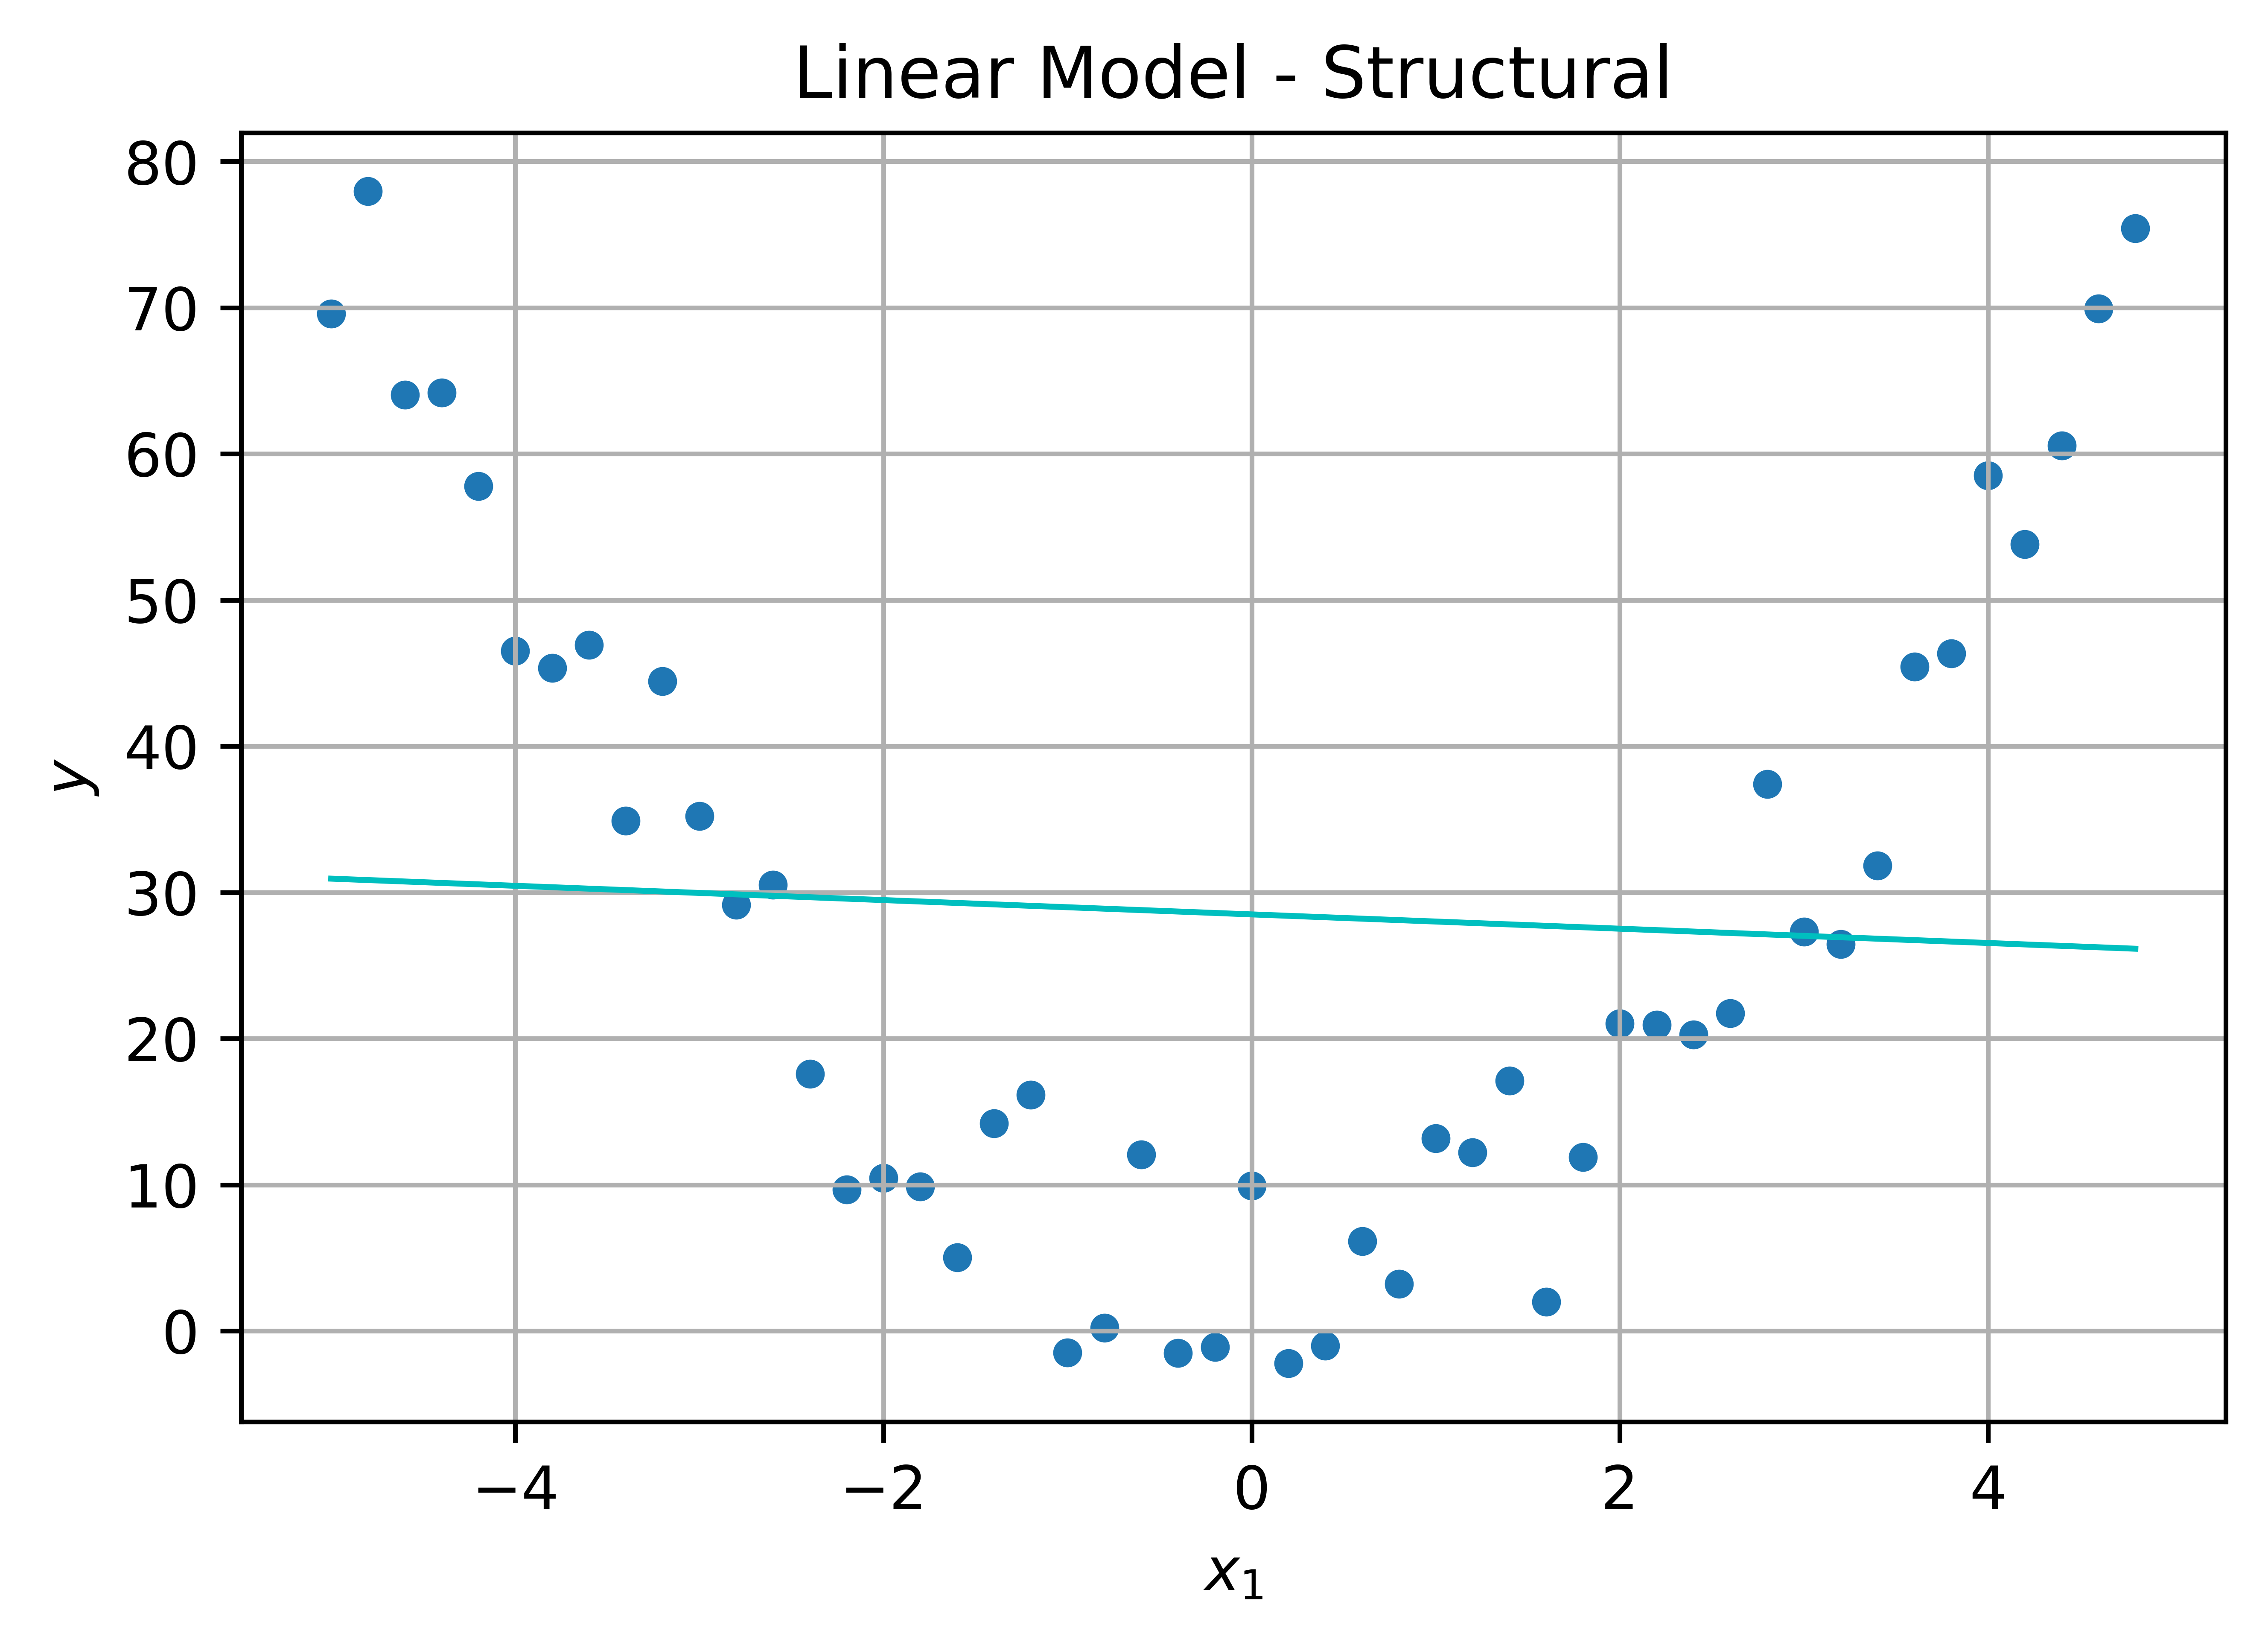
\includegraphics[width=70mm,scale=0.5]{images/regression_images/Structural_Linear_Model.png}

                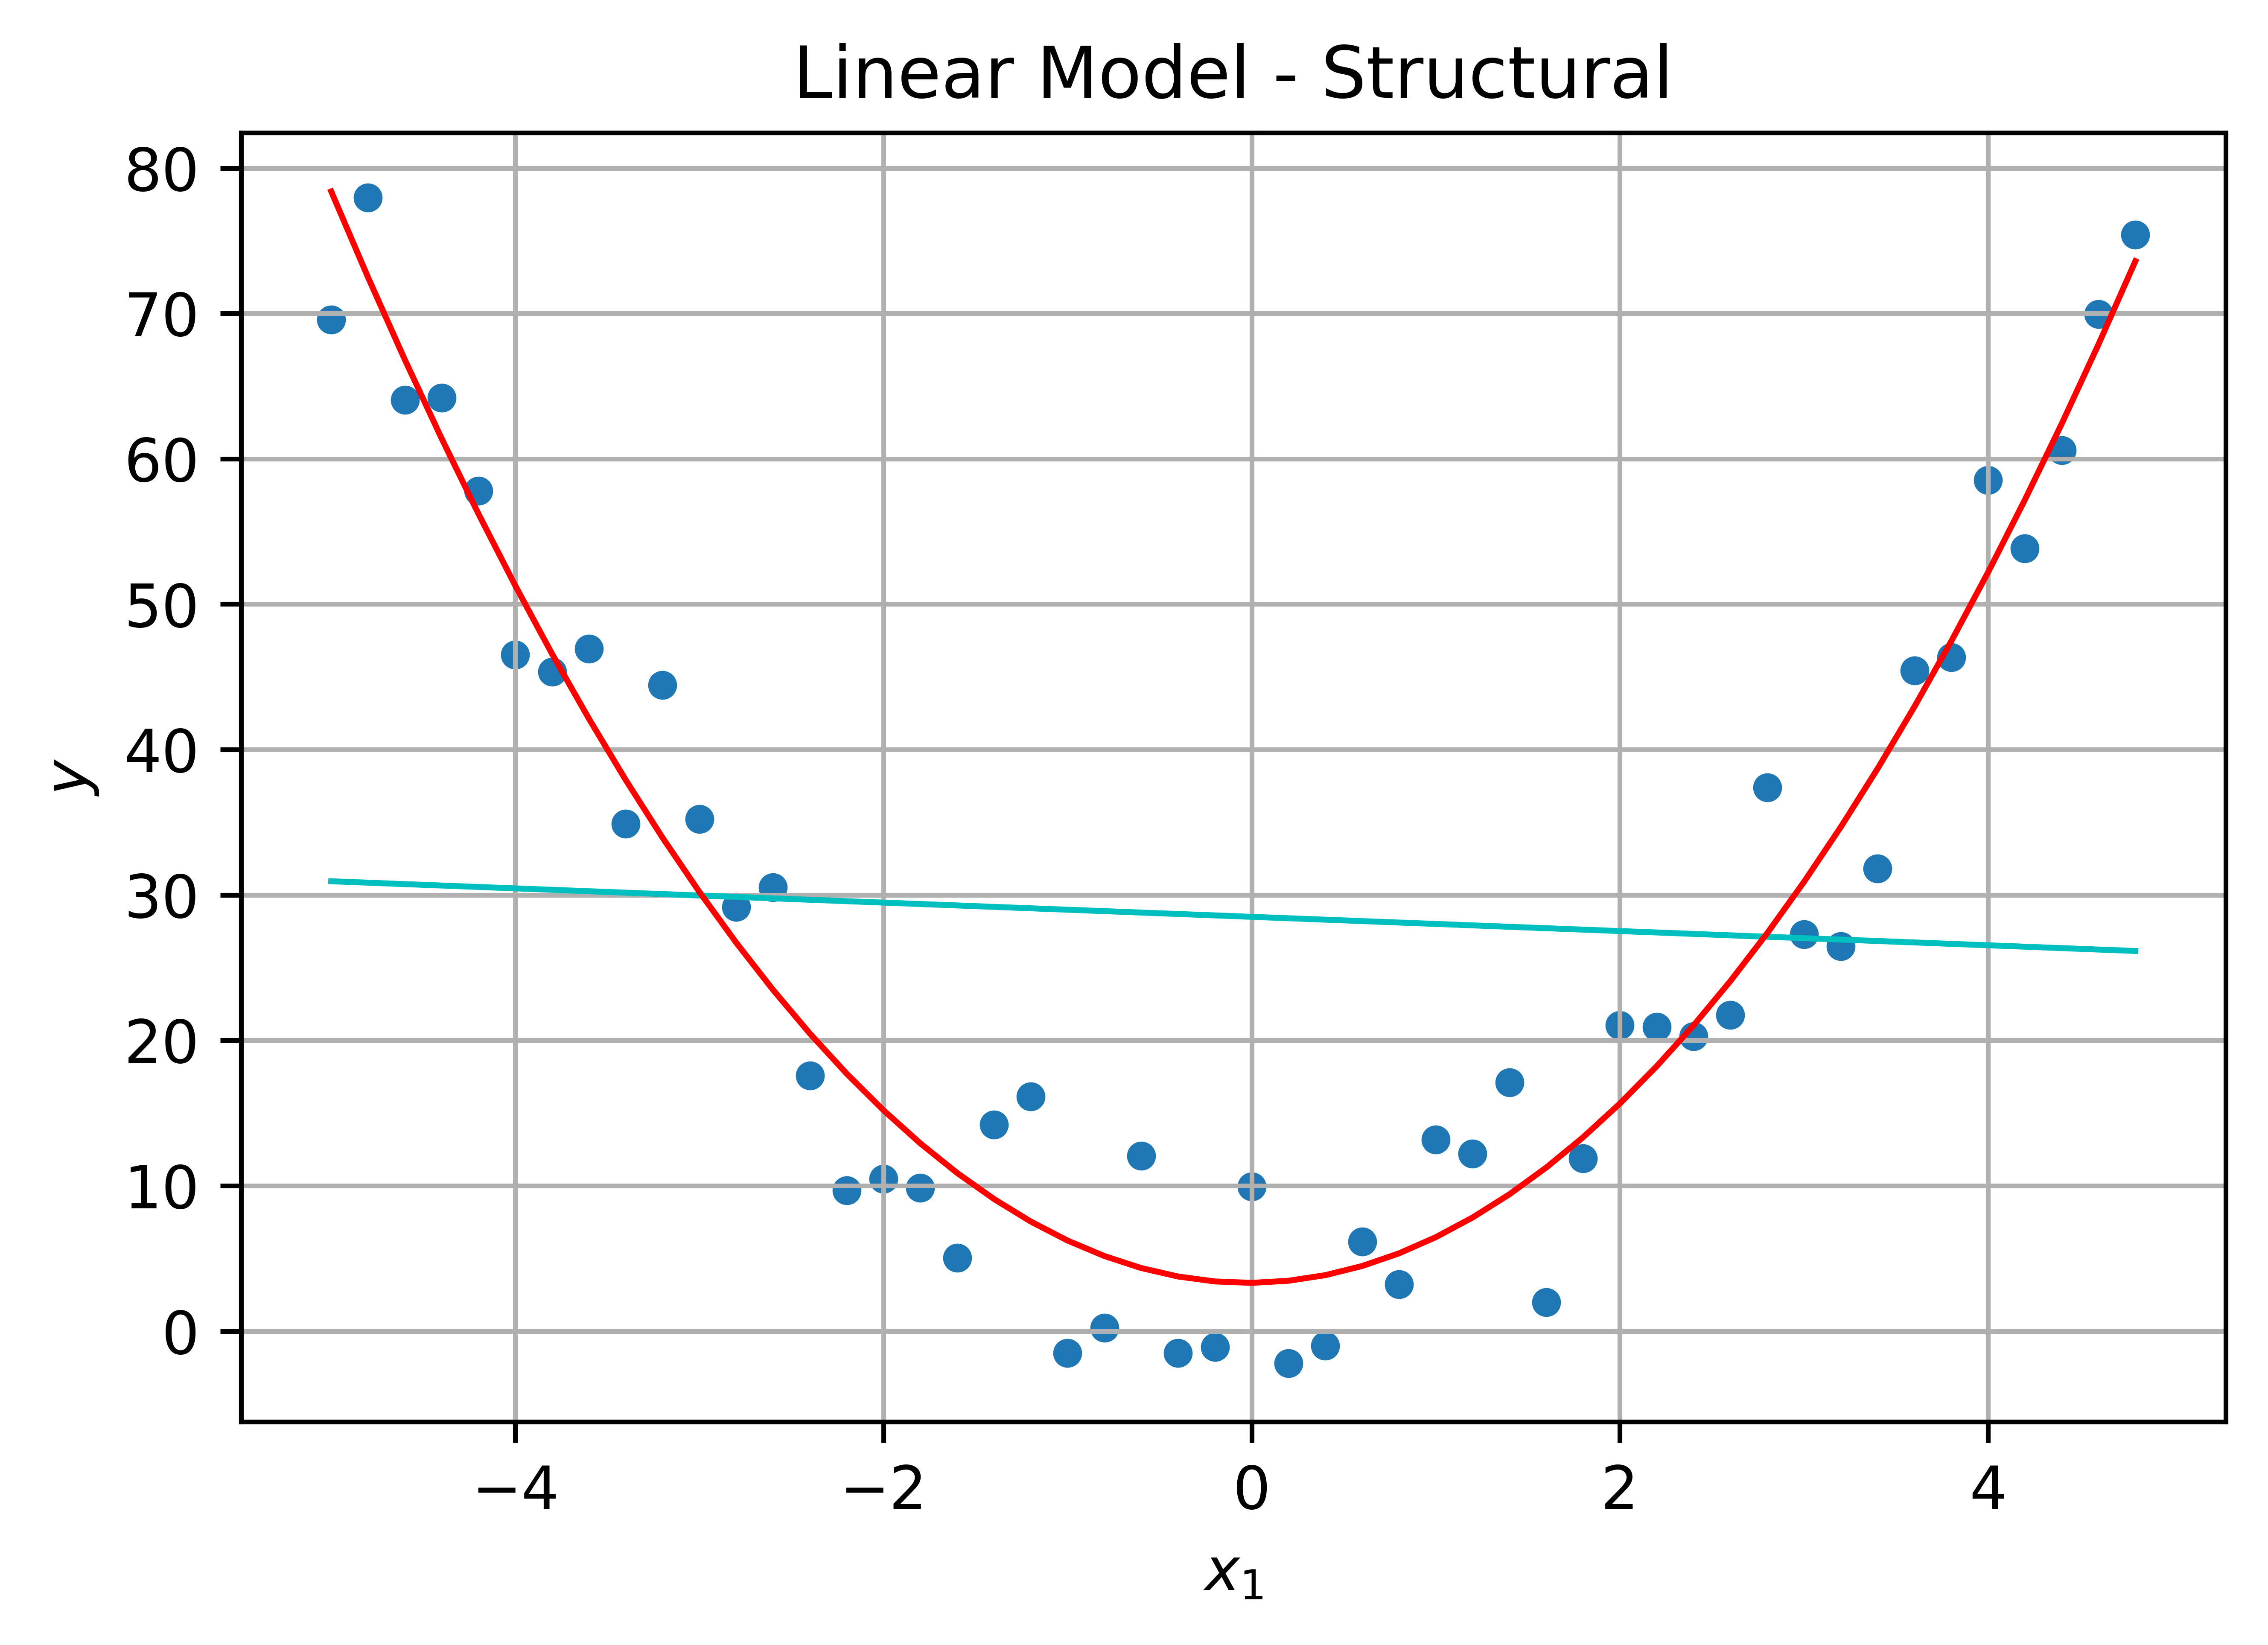
\includegraphics[width=70mm,scale=0.5]{images/regression_images/Structural_Quad_Model.png}

        
            \caption*{Our \textbf{linear} model isn't able to represent a quadratic function... so, we switch to a more \textbf{expressive} model: a \textbf{quadratic} equation.}
        \end{figure}
        
        \note{Remember that \textbf{expressiveness} is about how many possible models you have: if you have more models, you can solve more problems.}
        
        \begin{clarification}
           Note that $\lambda$ does not restrict our model class \purp{as severely} as \gren{switching polynomial order}, like above. 
        
            But, $\lambda$ \purp{limits} the use of larger $\theta$, which does make it \gren{unable} to solve some problems. So, the \purp{structural error} problem is similar.
        \end{clarification}
        
    \subsection{Tradeoffs of $\lambda$}
        
        Based on these two categories, we can discuss the tradeoffs of $\lambda$ more easily.
        
        As we mentioned, regularization \textbf{reduces} estimation error: 
        
        If we overfit to our current data, we are poorly \textbf{estimating} the distribution, because the training data may not perfectly \textbf{represent} it.\\
        
        \begin{concept}
            A \vocab{large $\lambda$} means \purp{more regularization}: we more strongly push for a more \gren{general} model, over a more \gren{specific} one.
            
            This results in...
            
            \begin{itemize}
                \item \gren{Reduced} estimation error
                \item \purp{Increased} structural error
            \end{itemize}
        \end{concept}
        
        However, \textbf{regularization} also \textbf{limits} the possible models we can use - those it views as less "general", it \textbf{penalizes}.
        
        That means the scope of possible models is \textbf{smaller} - some models are no longer \textbf{acceptable}. What if the only valid solution was in that space we \textbf{restricted}? Well, then we can't \textbf{find} it.
        
        That means there are certain \textbf{structural} limits on our model: that means that regularization \textbf{increases} structural error!\\
        
        \begin{concept}
            A \vocab{small $\lambda$} means \purp{less regularization}: we care less about a more \gren{general} model, allowing more \gren{specific} data to come into play.
            
            This results in...
            
            \begin{itemize}
                \item \purp{Increased} estimation error
                \item  \gren{Reduced} structural error
            \end{itemize}
        \end{concept}
        
    \subsection{Evaluating Hypotheses}
    
        So, we know that we have these \textbf{two} types of \textbf{error}. But it's \textbf{difficult} to \textbf{measure} them separately. 
        
        So instead, we just want to measure the \textbf{overall performance} of our hypothesis. 
        
        We do this using our \textbf{testing error}: this tells us how good our hypothesis is \textbf{after} training.
        
        \begin{equation}
            \testerr(h) =
            \frac{1}{m}  
            \sum_{i\purp{=n+1}}^{\purp{n+m}} 
                \left( 
                    h(\ex{x}{i}) - \ex{y}{i} 
                \right)^2
        \end{equation}
        
        Note that, before, we were using \textbf{regularization}. This is so we can \textbf{make} a more \textbf{general} model. 
        
        But here, we've \textbf{removed} it, because training is \textbf{done}: we're \textbf{not} going to make our hypothesis \textbf{better}. We just care about how \textbf{good} it came out.
        \note{We're already measuring the \textbf{generalizability} by using \textbf{new data}!}\\
        
        \begin{clarification}
            When we \vocab{evaluate a hypothesis} using \purp{testing error}, we are \gren{done training}: our hypothesis will not change.
            
            Because of this, we \textbf{do not} include the \purp{regularizer} when \gren{evaluating} our hypothesis.
        \end{clarification}
        
    \subsection{$\lambda$'s purpose: learning algorithms}
    
        Notice that we \textbf{removed} regularization when we were \textbf{evaluating} our hypothesis: regularization was used to \textbf{create} our hypothesis, but it is not \textbf{part} of that hypothesis.
        \note{Our hypothesis only includes the parameters $\Theta$: not $\lambda$!}
        
        That's because $\lambda$ is part of our \textbf{algorithm}: it determines how we run our algorithm. So, let's talk about that.\\
        
        \begin{definition}
            A \vocab{learning algorithm} is our procedure for \purp{learning} from data. It uses that data to create a \gren{hypothesis}. We can diagram this as:
            
            \begin{equation*}
                \data_n \longrightarrow 
                \boxed{\text{learning alg ($\hclass$)}} 
                \longrightarrow h
            \end{equation*}
            
            In a way, it's a function that takes in \gren{data} $\data_n$, and outputs a \purp{hypothesis} $h$.
        \end{definition}
        
        We're choosing \textbf{one hypothesis} $h$ from the hypothesis class $\hclass$: this is why $\hclass$ appears in the notation above.
        \note{We can write this as $h \in \hclass$}
        
    \subsection{Comparing Hypotheses and Learning Algorithms}
        
        We can take our learning algorithm
        
        \begin{equation*}
            \data_n \longrightarrow 
            \boxed{\text{learning alg ($\hclass$)}} 
            \longrightarrow h
        \end{equation*}
        
        And compare it to our hypothesis $h$:
        
        $$ x \rightarrow \boxed{h} \rightarrow y $$
        
        In a way, our learning algorithm is a function, that outputs another function!
        \note{This is similar to $\trainerr$, which instead \textbf{takes in} a function!}
        
        Our \textbf{hypothesis} can be adjusted with our \textbf{parameter} $\Theta$: if we change $\Theta$, we change our \textbf{performance}.
        
        Our \textbf{learning algorithm} depends on $\lambda$: so, it's like a \textbf{parameter}. But, it's different from $\Theta$: $\Theta$ \textbf{is} our model, $\lambda$ controls how we \textbf{choose} our model.
        
        So, it's a parameter ($\lambda$) that affects other parameters ($\Theta$). Because of that, we call it a \textbf{hyperparameter}.
        \note{It affects our hypothesis by pressuring it to have lower magnitude!}\\
        
        \begin{definition}
            \purp{Parameters} are \gren{variables} that adjust the behavior of \purp{our model}: our hypothesis.
            
            A \vocab{hyperparameter} is a \gren{variable} that can adjust \purp{how we make models}: our learning algorithm. 
        \end{definition}
        
        The \textbf{only} hyperparameter we have for now is $\lambda$, but the \textbf{development} of hyperparameters is an ongoing area of \textbf{research}.\\
        
        \begin{concept}
            \vocab{Lambda}, or $\lambda$, is a \vocab{hyperparameter}: it controls our \purp{learning algorithm.}
        \end{concept}
        
    \subsection{Evaluating our Learning Algorithm}
    
        So, while we can evaluate each \textbf{hypothesis}, it's also important to measure how our \textbf{learning algorithm} is performing.
        
        How do we measure it? Well, the job of our \textbf{learning algorithm} is to \textbf{pick good hypotheses}.\\
        
        \begin{concept}
            We can \vocab{evaluate} the performance of a \vocab{learning algorithm} using \purp{testing loss}: a good learning algorithm will create \gren{hypotheses} with \purp{low testing loss}.
        \end{concept}
        
        You could think of this as measuring the \textbf{skill} of a \textbf{teacher} (the learning algorithm) by the \textbf{success} of their \textbf{student} (the hypothesis) on a \textbf{test} (testing loss).
        
    \subsection{Validation: Evaluating with lots of data}
    
        When we were creating hypotheses, \textbf{randomness} caused some problems: you might not get \textbf{training data} that matched the \textbf{testing data} very well.
        
        The \textbf{same} can happen here, when \textbf{evaluating} your \textbf{algorithm}: maybe your model happened to create a bad (or unusually good!) hypothesis because of \textbf{luck}.
        
        The easy solution to \textbf{randomness} is to add \textbf{more data}: we get more \textbf{consistency} that way.
        
        So, we \textbf{repeatedly} get new training data and test data. For each, we \textbf{train} a different hypothesis. We can \textbf{average} their performance out, and use that to \textbf{estimate} the quality of our algorithm.\\
        
        \begin{definition}
            \vocab{Validation} is a way to \vocab{evaluate a learning algorithm} using \vocab{large amounts of data}.
            
            We do this by \gren{running} our algorithm \purp{many times} with new data, and \gren{averaging} the testing error of all the hypotheses.
            
            This process is often requires having \purp{lots of data} to train with, but is a \textbf{provably} good approach.
        \end{definition}
        
    \subsection{Our Problem: When data is less available}
        
        As mentioned, this takes up \textbf{lots of data}. What if we can't get as much: it's \textbf{expensive}, or not even possible? In this case, we have some \textbf{finite} data, $\data_n$. We \textbf{can't get more}.
        
        We solved the \textbf{randomness} problem by using \textbf{more} training and testing \textbf{data}. So, we need some way to \textbf{get} more \textbf{distinct} hypotheses.
        
        One set of data gives us one \textbf{hypothesis}. But, what if, rather than using \textbf{completely} new data, we used \textbf{slightly different} data each time?
        
        First, need to break $\data_n$ into a chunk for training, and a chunk for testing.
        
        \begin{figure}[H]
        \centering
            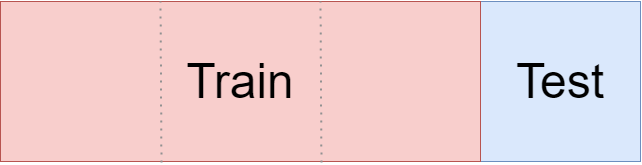
\includegraphics[width=70mm,scale=0.5]{images/regression_images/training_and_test_data.png}
        \end{figure}
        
        How do we get more hypotheses from this dataset?
        
    \subsection{Cross-Validation}
    
        We mentioned that we just want \textbf{different} hypotheses. Our hypotheses depend on our \textbf{training data}. So we want to \textbf{change} our training data.
        
        We can't \textbf{add} data to it, because then we \textbf{lose} testing data. We shouldn't \textbf{remove} data, because then we're just making a hypothesis that's \textbf{less well-informed}.
        
        Instead, we'll \textbf{swap} some of the training data for testing data.
        
        \begin{figure}[H]
        \centering
            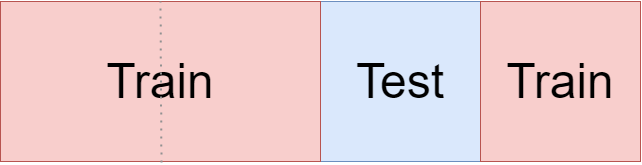
\includegraphics[width=70mm,scale=0.5]{images/regression_images/training_and_test_data_2.png}
        \end{figure}
        
        This will create a new hypothesis, and the data is partially different! In fact, we can do this for each of our chunks:
        
        \begin{figure}[H]
                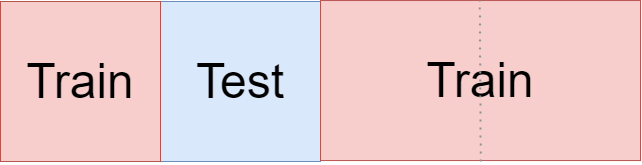
\includegraphics[width=70mm,scale=0.5]{images/regression_images/training_and_test_data_3.png}
                
                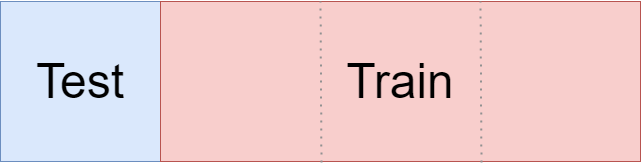
\includegraphics[width=70mm,scale=0.5]{images/regression_images/training_and_test_data_4.png}
            
        \end{figure}
        
        We now have \textbf{four different hypotheses} for the price of one!\\
        
        \begin{definition}
            \vocab{Cross-validation} is a way to \vocab{evaluate a learning algorithm} using \vocab{limited data}.
            
            We do this by \purp{breaking} our data it into \gren{chunks} to create \purp{multiple hypotheses} from one dataset.
            
            For each \gren{chunk}, we train one dataset on all the data \textbf{not in that chunk}. We get our \purp{test error} using the chunk \textbf{we left out}.
            
            For $k$ chunks, we end up with $k$ hypotheses. By \gren{averaging} out their performance, we can \purp{approximate} the quality of our algorithm.
        \end{definition}
        
        This approach is much \textbf{less expensive}, and very common in machine learning! But, some of the theoretical \textbf{benefits} of validation are not \textbf{proven} to be true for cross-validation.\\
        
        \begin{clarification}
            Note that the goal of validation and cross-validation is \textbf{not} to evaluate \purp{one hypothesis}.
            
            Instead, it is instead meant to evaluate a \purp{learning algorithm}. This is why we have to create \purp{many} hypotheses: we want to see that our algorithm is \gren{generally} good!
        \end{clarification}
        
    \subsection{Hyperparameter Tuning}
    
        Now, we know how to \textbf{evaluate} a learning algorithm, just like how we \textbf{evaluate} a hypothesis. 
        
        Once we knew how to evaluate a hypothesis, we started \textbf{optimizing} our parameters for the \textbf{best} hypothesis. So, we could do the same for our \textbf{learning algorithm}.
        
        Each $\lambda$ value creates a slightly \textbf{different} learning algorithm: we can \textbf{optimize} this \textbf{hyperparameter} to create the \textbf{best} learning algorithm.
        
    \subsection{How to tune our algorithm}
    
        When we were \textbf{optimizing} our hypothesis, we started by \textbf{randomly} trying hypotheses. Then, we used an \textbf{analytical} approach.
        \note{By "analytical", we mean directly creating an equation, and solving it.}
        
        We don't always have \textbf{simple} equations to work with: with all of our data, it's hard to come up with \textbf{manageable} equations. So, we \textbf{won't} try doing it \textbf{analytically}.
        
        So, we could \textbf{randomly} try $\lambda$ values and pick the \textbf{best} one. This is pretty \textbf{close} to what we usually end up doing. For each value we pick, we'll use \textbf{cross-validation} to evaluate.
        
        For now, we'll systematically go through $\lambda$ values: $\lambda=.1, .2, .3 \dots$\\
        
        \begin{concept}
            \vocab{Hyperparameter tuning} is how we \purp{optimize} our \gren{learning algorithm} to create the \purp{best} hypotheses.
            
            The simplest way to do this is to try \gren{multiple} different values of $\lambda$. For each value, we use \gren{cross-validation} to evaluate that learning algorithm.
            
            Finally, we pick whichever $\lambda$ gives you the \purp{best} algorithm, and thus the \purp{best} hypotheses.
        \end{concept}
        
    \subsection{Hyperparameter Tuning: Two kinds of optimization}
    
        There's something often \textbf{confusing} about hyperparameter tuning to students:
        
        When we're \textbf{optimizing} $\lambda$, we have to determine the quality of \textbf{each} learning algorithm.
        
        But, to get the \textbf{quality} of that algorithm, we have to optimize $\Theta$ based on that \textbf{single} learning algorithm.
        \note{If we do cross-validation, then we have to optimize $k$ times!}
        
        That means, \textbf{every time} we try a different $\lambda$ value, we have to do one optimization problem. But trying different $\lambda$ values is a \textbf{different} kind of optimization.
        
        That means we have \textbf{two layers} of optimization!\\
        
        \begin{clarification}
            We \purp{optimize} $\lambda$ by trying many values.
            
            But, for each $\lambda$ value, we have to \gren{optimize} $\Theta$.
            
            So, we have to optimize $\Theta$ \purp{repeatedly} in order to optimize $\lambda$ \purp{once}! This gives us $\lambda^*.$
        \end{clarification}
        
        But, our goal is to get a \textbf{hypothesis}. So we use that $\lambda^*$ to, finally, get our $\theta^*$
        
    \subsection{Pseudocode Example}
        
        This technique is \textbf{not} limited to regression. Thus, we'll be a bit more \textbf{general}: we won't assume an \textbf{analytical} solution. Instead, we \textbf{optimize} by just trying different $\Theta$ values.
        
        We can represent this in pseudocode:
        \note{If this pseudocode isn't helpful to you, don't worry! Some students like it, some don't.}
        
        \begin{codebox}
            \Procname{$\proc{Lambda-Optimization}
                       (\data, lambda\_values, theta\_values)$}
                       
                \li \For $\lambda$ \In $lambda\_values$        
                \qquad\quad\#Try lambda values
                
                \li     \Do \For $\Theta$ \In $theta\_values$  
                \qquad\quad\#Try theta values    
                            \Do

                                \li Calculate $J(\Theta)$    
                                \qquad\qquad\qquad\#Compare values
                            \End
                        
                        \li Choose best theta value $\Theta^*$ 
                        \quad\#Best for each lambda

                        \End
                \li Choose best lambda value $\lambda^*$
                \li
                    
                \li \Return $\lambda^*$
        \end{codebox}
        
    To reiterate: this $\lambda^*$ will then we used to get our final result, $\theta^*$.
        
\section{Terms}

    \begin{itemize}
        \item Hypothesis
        \item Theta ($\Theta$)
        \item Input Space
        \item Regression
        \item Feature
        \item Feature Transformation
        \item Training Error
        \item Test Error
        \item Objective Function
        \item Min function
        \item Argmin function
        \item Star Notation ($\theta^*$)
        \item Linear Regression
        \item Hypothesis Class
        \item Square Loss
        \item Ordinary Least Squares (OLS) Problem
        \item OLS Objective Function
        \item Hyperplane
        \item Weight
        \item Input Matrix
        \item Output Matrix
        \item Gradient
        \item OLS Solution
        \item Regularization
        \item Regularizer
        \item Regularizer for Regression
        \item Lambda ($\lambda$)
        \item Ridge Regression
        \item RR Objective Function
        \item RR Solution
        \item Invertibility
        \item Estimation Error
        \item Structural Error
        \item Expressiveness
        \item Learning Algorithm
        \item Hyperparameter
        \item Validation
        \item Cross-Validation
        \item Chunk (Cross-Validation)
        \item Hyperparameter Tuning
    \end{itemize}
        
        
        






%%% Local Variables:
%%% mode: latex
%%% TeX-master: "top"
%%% End:
